\documentclass[12pt,openright,twoside]{report}
\usepackage[a4paper,top=25mm,bottom=25mm,right=25mm,left=25mm,bindingoffset=6mm]{geometry}
\usepackage[utf8]{inputenc}
\usepackage[dutch]{babel}
\usepackage{amsmath}
\usepackage{graphicx}
\usepackage[dvipsnames]{xcolor}
\usepackage{pict2e}
\usepackage{tabu}
\usepackage{booktabs}
%\usepackage{bookmark,hyperref}
\usepackage[hypertexnames=true]{hyperref}
%\usepackage{hyperref}
\usepackage{gensymb}
\usepackage{wrapfig}
\usepackage{multirow}
\usepackage[nottoc]{tocbibind}

\usepackage{xcolor}
\usepackage{colortbl}
%\usepackage[table]{xcolor}
%\usepackage{tabularray}
\usepackage{watermark}
\usepackage{wallpaper}
\usepackage{eurosym}
\usepackage[toc,title,page]{appendix}
\usepackage{courier}
\usepackage{listings} 
\usepackage{enumitem}
\usepackage{url}
\usepackage{soul}
\usepackage{comment}
\usepackage{parskip}
\usepackage{etoolbox}
\usepackage{textcomp}
\usepackage{float}
%\usepackage{lststyle-VS2017.sty}

%\usepackage{minted} 


%\usepackage{fontspec}
\graphicspath{{figuren/}}


\definecolor{mygray}{gray}{0.85}

% Vanaf hier: Gert
\definecolor{codegreen}{rgb}{0,0.6,0}
\definecolor{codegray}{rgb}{0.5,0.5,0.5}
\definecolor{codepurple}{rgb}{0.58,0,0.82}
\definecolor{backcolour}{rgb}{0.95,0.95,0.92}

\lstdefinestyle{bash}{
	language=bash,
	backgroundcolor=\color{backcolour},   
	commentstyle=\color{codegreen},
	keywordstyle=\color{magenta},
	numberstyle=\tiny\color{codegray},
	stringstyle=\color{codepurple},
	basicstyle=\ttfamily\footnotesize,
	breakatwhitespace=false,         
	breaklines=true,                 
	captionpos=b,                    
	keepspaces=true,                 
	numbers=left,                    
	numbersep=5pt,                  
	showspaces=false,                
	showstringspaces=false,
	showtabs=false,                  
	tabsize=2
}
% Tot hier: Gert

\newcommand{\ctext}[3][RGB]{%
	\begingroup
	\definecolor{hlcolor}{#1}{#2}\sethlcolor{hlcolor}%
	\hl{#3}%
	\endgroup
}


\newcommand{\specialcell}[2][c]{%
	\begin{tabular}[#1]{@{}c@{}}#2\end{tabular}}

\newcommand*{\img}[1]{%
	\raisebox{-.3\baselineskip}{%
		\includegraphics[
		height=\baselineskip,
		width=\baselineskip,
		keepaspectratio,
		]{#1}%
	}%
}
\newcommand*{\imgl}[1]{%
	\raisebox{-.3\baselineskip}{%
		\includegraphics[
		height=\baselineskip,
		%		width=\baselineskip,
		keepaspectratio,
		]{#1}%
	}%
}

%Formatering av rubriker
%%%%%%%%%%%%%%%%%%%%%%%%%%%%%%%%%%%%%%%%%%%%%%%%%%%%%%%%%%%%%%%%%%%%%%%%%%%%%%%%%%%%%%%
\usepackage{titlesec, blindtext, color}
\titleformat{\chapter}[hang]{\Huge\bfseries}{\thechapter}{20pt}{}{}
\titlespacing*{\chapter}{0pt}{*0}{*3}
\titlespacing*{\section}{0pt}{*4}{*1}
\titlespacing*{\subsection}{0pt}{*3}{*0}
\titlespacing*{\subsubsection}{0pt}{*4}{*1}

\setcounter{secnumdepth}{2}
\setcounter{tocdepth}{2}
%%%%%%%%%%%%%%%%%%%%%%%%%%%%%%%%%%%%%%%%%%%%%%%%%%%%%%%%%%%%%%%%%%%%%%%%%%%%%%%%%%%%%%%

\usepackage{tocloft} %Control the ToC formatting

\setlength{\parindent}{0pt}
\setlength{\parskip}{1em}

\lstset{ 
	basicstyle=\ttfamily\footnotesize,
	language=C++,
	        keywordstyle=\color{blue},
	stringstyle=\color{red},
	commentstyle=\color{green},
	morecomment=[l][\color{magenta}]{\#},
    captionpos=b,
	breaklines=true,    % Gert 
    tabsize=3
}


%Formatting of page numbering (Comment to have the number centered)
%%%%%%%%%%%%%%%%%%%%%%%%%%%%%%%%%%%%%%%%%%%%%%%%%%%%%%%%%%%%%%%%%%%%%%%%%%%%%%%%%%%%%%%
\usepackage{fancyhdr}
\pagestyle{fancyplain}%
\fancyhf{} % clear all header and footer fields
\fancyfoot[RO,LE]{\thepage}
\renewcommand{\headrulewidth}{0pt}
%%%%%%%%%%%%%%%%%%%%%%%%%%%%%%%%%%%%%%%%%%%%%%%%%%%%%%%%%%%%%%%%%%%%%%%%%%%%%%%%%%%%%%%


\usepackage[font=footnotesize,format=plain,labelfont=bf,textfont=sl]{caption}
\usepackage[labelformat=simple,font=footnotesize,format=plain,labelfont=bf,textfont=sl]{subcaption}

\hypersetup{
	colorlinks=true,
	linkcolor=blue,
	filecolor=magenta,      
	urlcolor=cyan,
	pdfnewwindow=true, 
}
%opening
%  \date{\today}
\date{}
\title{
	
	{\vspace{-4cm}}
	
	{\hspace{-20pt}\begin{bfseries}\LARGE{\color{black}Object Georiënteerd Programmeren  \\~ \\ ~~~~~~~~ ( Introductie )} \end{bfseries}  } 
	~\newline ~\newline
	\small{(Practicumhandleiding inclusief de practicumopstelling voor de RockPi)}
	\ThisCenterWallPaper{0.8}{figuren/frontRock.png}
	
	%{\hspace{-20pt}\begin{bfseries}\Huge{\color{black} Realtime programmeren} \end{bfseries}  } \\
		%{(practicumopdracht Mbed)}\\
	{Versie 0.6}
	%\ThisCenterWallPaper{0.9}{figuren/voorpagina.png}
	
	%	\vfill	
	{\vspace{12cm}}	
	{\color{white}  
		\raggedleft  \par}
	
}



\begin{document}
	
	
	\maketitle
	
	\tableofcontents
	
	\let\cleardoublepage\clearpage
	
	\chapter{Inleiding}\label{chap:inl}
Voor het practicum OOPR1 zijn (ongeveer) 25 RockPi’s beschikbaar. Dit zijn Raspberry Pi achtige ‘Single Board Computers’ die met een Linux variant werken, in dit geval Debian 10. De RockPi’s zijn aangeschaft omdat Raspberry Pi’s niet leverbaar (of te duur) waren.
Tijdens het practicum gebruik je een RockPi van school. Je kunt deze alleen op school gebruiken, je mag hem niet meenemen naar huis. Dat is dan ook het belangrijkste nadeel.

Het gebruik van de RockPi heeft een aantal voordelen:
\begin{itemize}
\item Je hoeft zelf niets aan te schaffen
\item Je werkt onder gecontroleerde omstandigheden: de verstrekte RockPi bevat alles wat nodig is voor het practicum. Dat betekent dat jij- of de docent niet eerst moet puzzelen om de omgeving aan de praat te krijgen.
\end{itemize}

\hypertarget{USBinleiding}{}
Bij het practicum heb je \textit{je eigen} USB stick nodig om je bestanden op te zetten (\textit{geen gedeelde!}). Een USB stick van 1GB is goed genoeg (128+ MB). Groter mag, maar is zinloos.
\begin{itemize}
\item Je werkt op je eigen \hyperlink{chp:USBstick}{USB stick} en niet op het bestandssysteem van de RockPi. 
\item Na afloop van het practicum lever je de RockPi in zonder daar bestanden op achter te laten. 
\item Ga er vanuit dat de RockPi’s na een practicum gewist worden!
\end{itemize}
\colorbox{yellow}{\textcolor{red}{\textbf{\textit{Dit is géén security practicum, de RockPi's zijn slecht beveiligd.}}}}\\
\colorbox{yellow}{\textcolor{red}{\textbf{\textit{Ga dus niet klooien en klieren op de RockPi van iemand anders.}}}}\\
\colorbox{yellow}{\textcolor{red}{\textbf{\textit{Als je overlast veroorzaakt zal de docent je uit het practicum verwijderen!!}}}}

\section{Voorbereiding - Software installeren}
Zorg dat je vóór het practicum de benodigde software geïnstalleerd hebt.
Zie Bijlage \ref{app:instal} voor software installatie.
\newpage

\begin{comment}
\begin{itemize}
\item Installeer Github Desktop: \url{https://desktop.github.com/}
\item Vanuit Github Desktop, druk Ctrl+Shift+O voor 'Clone repository' en voeg de repository \textbf{JohnVi-hhs/oop} toe.
\item Installeer 'Visual Studio Code' (VSC) volgens de instructies in \newline \url{https://github.com/Grrtzm/OOPR1} \textit{(moet nog aangepast worden)}
\item Download en installeer de VNC viewer:  \newline \url{https://www.realVNC.com/en/connect/download/combined/}
\item (Optioneel maar wel handig) Download en installeer de SSH client KiTTY  \newline \url{https://www.fosshub.com/KiTTY.html} \newline
KiTTY is een opvolger van PuTTY. Het grote voordeel is dat KiTTY automatisch opnieuw verbinding maakt als de verbinding even verbroken is geweest.
\end{itemize}
\end{comment}

\section{Eerste gebruik van de RockPi}
We gaan er van uit dat je de RockPi in lokaal D2.001 of D2.003 van HHS Delft gebruikt. \newline
De RockPi is al ingesteld voor Wi-Fi netwerk in D2.001: \textbf{Lab001}. \newline
Log ook met je laptop in op dit netwerk. Het password is \textbf{Lab001WiFi}. \newline
In Figuur \ref{fig:netw} wordt weergegeven hoe de RockPi op het lab netwerk is aangesloten.
\begin{figure}[h!]
	\centering
	\begin{center} 	
		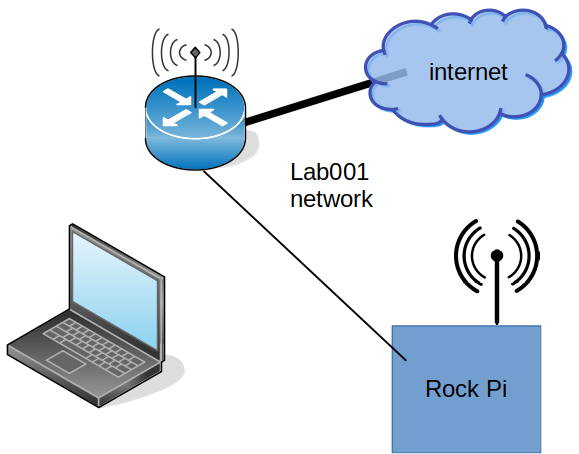
\includegraphics[width=0.4\textwidth]{figuren/laBnetwork}
		\caption{De RockPi in het lab netwerk}
		\label{fig:netw}   
	\end{center}
\end{figure}
\break
Sluit de USB-C voedingskabel aan zodat de RockPi gaat opstarten (op de RockPi gaat een groene led branden). Verder hoef je nog niets aan te sluiten!
\begin{figure}[h!]
	\centering
	\begin{center} 	
		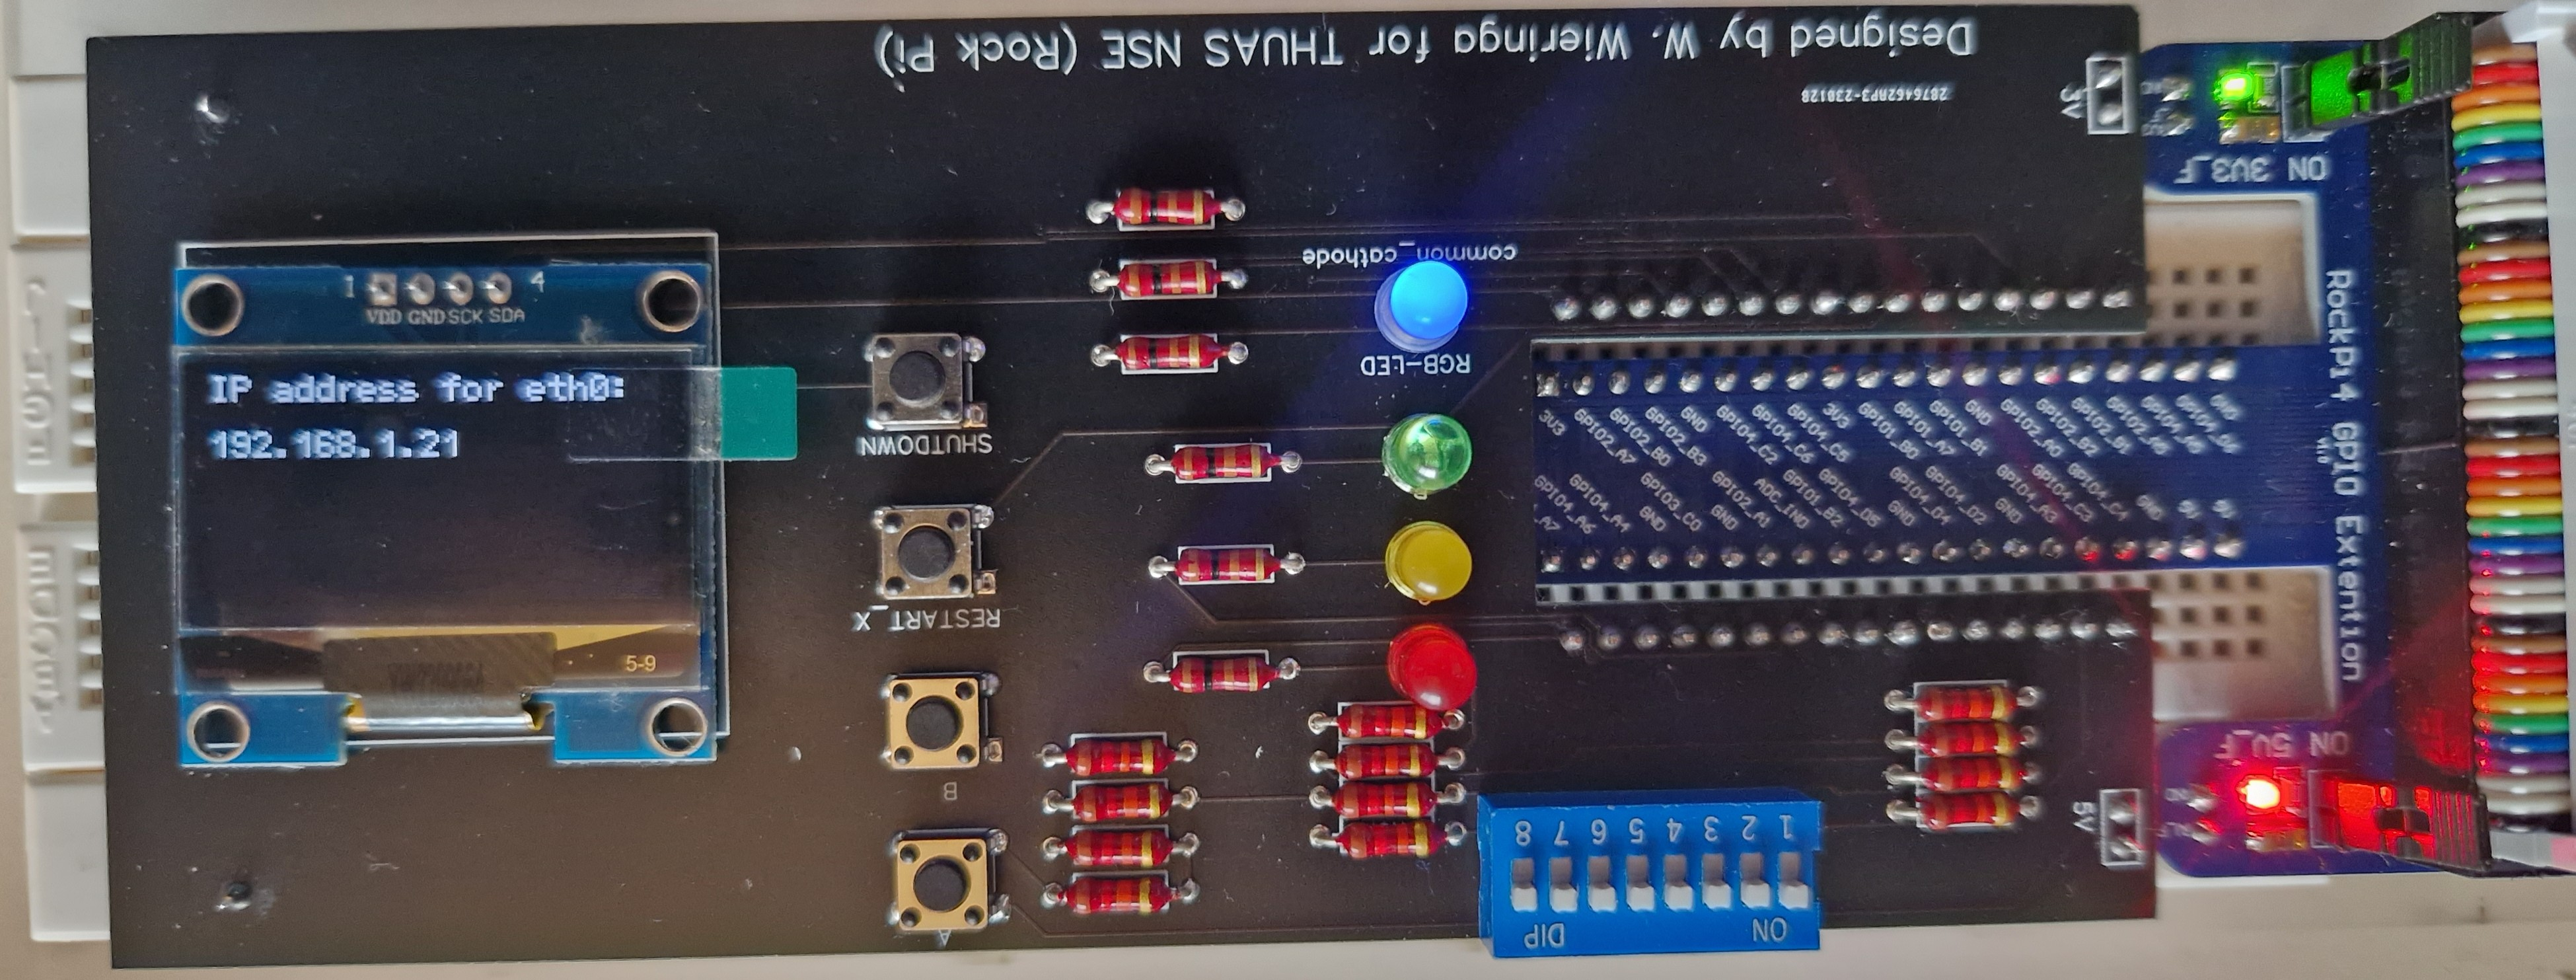
\includegraphics[width=1\textwidth]{figuren/rockIPnr}
		\caption{Het uitbreidingsbord van de RockPi}
		\label{fig:rockIPnr}   
	\end{center}
\end{figure}

\textbf{\textit{Controleer de zelftest:}} Om zeker te weten dat het bovenstaande bordje OK is gaat de RockPi alle leds even aan en uitzetten. \newline
Als je de RockPi in het lab (D2.001) aanzet, verschijnt op het oled display 
% bij “IP address for wlan0:”
een IP adres van het Lab001 Wi-Fi netwerk (zie Figuur \ref{fig:rockIPnr}). %\newline
Nu kun je via \hyperlink{chp:ssh}{SSH} en/of \hyperlink{chp:vnc}{VNC} een verbinding maken met dit IP adres en inloggen op de RockPi.
% wijziging 15-4-2023
%De username is \textbf{rock}, het password is ook \textbf{rock}. Mocht er een sudo password gevraagd worden, dan is dit ook \textbf{rock}.

De username is \textbf{rock}, het password voor deze sessie wordt weergegeven op het display, zie Figuur \ref{fig:rockIPnr} (elke keer als de RockPi opnieuw opstart krijg je een nieuw password). Mocht er een sudo password gevraagd worden, dan is dit hetzelfde password.

Overigens kun je ook een ethernet kabel aansluiten.
% zoals in Figuur \ref{fig:rockIPnr} te zien is bij “IP address for eth0:”.\break\newline
Zorg wel dat je PC op hetzelfde netwerk is aangesloten. Als VNC het niet wil doen, maar SSH wel, dan zitten je PC en de RockPi mogelijk op verschillende Wi-Fi access-points. Als VNC niet werkt, maar je RockPi en laptop zitten wel op hetzelfde netwerk, dan kun je het knopje '\textbf{Restart\_X}' indrukken, dit herstart de grafische schil op de RockPi.

Zodra je bent ingelogd met VNC, kun je je USB stick aansluiten en configureren. Het maakt niet uit welke USB poort je gebruikt. 

Als je klaar bent met je practicum, moet je de RockPi netjes afsluiten. Door op het knopje ‘\textbf{Shutdown}’ te drukken, wordt het operating system netjes afgesloten zodat het bestandssysteem niet corrupt raakt (wat kan gebeuren als je de RockPi gewoon uitzet).

'Knop\_A' kun je gebruiken om tijdens het opstarten voor volledig GPIO gebruik te kiezen; druk de knop in vóórdat je de RockPi aanzet, en houd hem ingedrukt tot de LED zelftest klaar is. Dit is zo gedaan omdat wisselen tussen PWM gebruik (voor de rode en blauwe leds van de driekleuren led) en GPIO (alleen aan en uit, geen ‘analoge’ waarden) niet lukt zonder opnieuw op te starten.

Aan 'Knop\_A', 'Knop\_B' en de DIP switches (blauwe blokje) zijn verder geen functies toegewezen. Daar kun je zelf code voor schrijven.

\section{Inloggen met VNC}
Controleer even of het werkt. Je gaat dit later pas gebruiken. \\Voer het IP adres zoals getoond op het oled display in op \hyperlink{chp:vnc}{VNC}  (Figuur \ref{fig:rockIPnr}).\newline
Log in op de RockPi en klik op het ‘Terminal’ icoon (rood omcirkeld in Figuur \ref{fig:termico}):
\begin{figure}[h!]
	\centering
	\begin{center} 	
		
\includegraphics[width=0.4\textwidth]{figuren/Terminal-icoon}
		\caption{Terminal icoon}
		\label{fig:termico}   
	\end{center}
\end{figure}

Nu verschijnt het Terminal venster. Van hieruit kun je allerlei commando's invoeren (en tegelijk wordt o.a. schermresolutie ingesteld en wordt de screensaver uitgezet):
\begin{figure}[h!]
	\centering
	\begin{center} 
		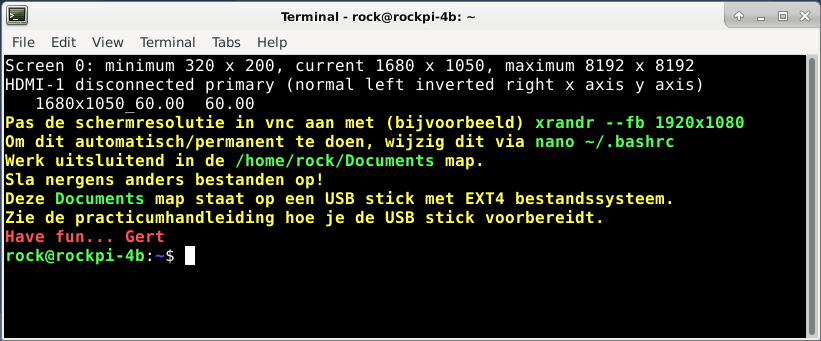
\includegraphics[width=0.9\textwidth]{figuren/terminal-inlogscherm}	
		\caption{Het Terminal scherm}
		\label{fig:terminal-inlogscherm}   
	\end{center}
\end{figure}

\hypertarget{chp:USBstick}{}
\section{USB Stick voorbereiden}
\textbf{\textit{LET OP!! }}
\begin{itemize}
	\item Met onderstaande procedure verwijder je alle bestanden van je USB stick!
	\item Je hebt genoeg aan een \hyperlink{USBinleiding}{kleine USB stick} (ergens tussen 128MB en 4 GB).
	\item Je kunt hierna alléén met Linux op je USB stick kijken, niet meer met Windows!
\end{itemize}

Formatteer nu je USB stick met EXT4 filesystem. Dit is nodig omdat Linux d.m.v. attributen in het bestandssysteem aangeeft of een bestand uitvoerbaar (‘executable’) is. Dat is op  een Windows compatible USB stick (met FAT of NTFS bestandsysteem) niet mogelijk.
Kijk of je USB stick gezien wordt. Geef het commando \textbf{\texttt{lsblk}} en kijk of daar een device bij zit met sda in de naam (zie hieronder in de listing van \texttt{lsblk}). In dit geval is deze er. De partitie waar we gebruik van maken is /dev/sda1.

\begin{lstlisting}[language=bash]
rock@rockpi-4b:~$ lsblk
NAME         MAJ:MIN RM   SIZE RO TYPE MOUNTPOINT
sda            8:0    1   1.9G  0 disk
`-sda1         8:1    1   1.9G  0 part /media/rock/9C02-C2F1
mmcblk1      179:0    0 115.2G  0 disk
|-mmcblk1p1  179:1    0   3.9M  0 part
|-mmcblk1p2  179:2    0     4M  0 part
|-mmcblk1p3  179:3    0     4M  0 part
|-mmcblk1p4  179:4    0   512M  0 part
`-mmcblk1p5  179:5    0   7.8G  0 part /
mmcblk1boot0 179:32   0     4M  1 disk
mmcblk1boot1 179:64   0     4M  1 disk
mmcblk1rpmb  179:96   0     4M  0 disk
}
\end{lstlisting}
	
\underline{\textbf{Controle:}}\newline 
Als je het commando \href{https://www.techrepublic.com/article/linux-101-what-is-the-mount-command-and-how-do-you-use-it/}{\textbf{\texttt{mount}}} geeft, dan verwacht je in de uitvoer het device (de disk) /dev/sda1 te zien: % \textbf{\texttt{mount}}
\begin{lstlisting}
/dev/sda1 on /media/rock/9C02-C2F1 type vfat (rw,nosuid,nodev,relatime,uid=1000,gid=1000,fmask=0022,dmask=0022,codepage=936,iocharset=utf8,shortname=mixed,showexec,utf8,flush,errors=remount-ro,uhelper=udisks2)
\end{lstlisting}

Hierboven zie je dat disk ge-'mount' is. Om te formatteren moet je eerst 'umount' doen:\newline
\textbf{\texttt{umount /dev/sda1 }}\newline
Nu USB disk formatteren met ext4 filesystem (het \textit{sudo} password is hetzelfde als het password van user \textit{rock}; het password van het display):\newline
\textbf{\texttt{sudo mkfs -t ext4 /dev/sda}}\newline
Vervolgens disklabel 'Documents' instellen:\newline
\textbf{\texttt{sudo e2label /dev/sda Documents}}\newline
Trek nu de USB stick uit de RockPi en steek hem terug zodat deze ge-'mount' wordt onder de naam 'Documents'.\\
Als laatste gebruiker \textit{rock} eigenaar maken van de USB stick:\newline
\textbf{\texttt{sudo chown rock /home/rock/Documents}}\newline

Hieronder zie je de output van bovenstaande commando's:
	
\begin{lstlisting}[language=C]   % Gert: Is het niet, maar hiermee doet hij geen speciale opmaak
rock@rockpi-4b:~\$ umount /dev/sda
umount: /dev/sda#: No such file or directory
rock@rockpi-4b:~\$ sudo mkfs -t ext4 /dev/sda
mke2fs 1.44.5 (15-Dec-2018)
/dev/sda contains a vfat file system
Proceed anyway? (y,N) y
Creating filesystem with 491520 4k blocks and 123120 inodes
Filesystem UUID: 1b2275ec-6dbd-4f3b-8d41-feaf4da0c7b7
Superblock backups stored on blocks:
32768, 98304, 163840, 229376, 294912

Allocating group tables: done
Writing inode tables: done
Creating journal (8192 blocks): done
Writing superblocks and filesystem accounting information: done
\end{lstlisting}

Als het formatteren en labelen klaar is, kun je testen of de USB stick correct gezien wordt:\newline
Verwijder de USB stick, wacht even en steek hem weer terug in een USB poort.\newline
Klik in VNC op het ‘File Manager’ icoon (rood omcirkeld in Figuur \ref{fig:fileman}):

\begin{figure}[h!]
	\centering
	\begin{center} 	
		
\includegraphics[width=0.4\textwidth]{figuren/File-Manager}
		\caption{Terminal icoon}
		\label{fig:fileman}   
	\end{center}
\end{figure}
Ga in de ‘File Manager’ naar het ‘Documents’ device.\newline
Als dit werkt, dan zie je onderin de statusbalk van de ‘File Manager’ hoeveel vrije ruimte je USB stick heeft (rood omcirkeld in Figuur \ref{fig:fileman})

\begin{figure}[h!]
	\centering
	\begin{center} 	
		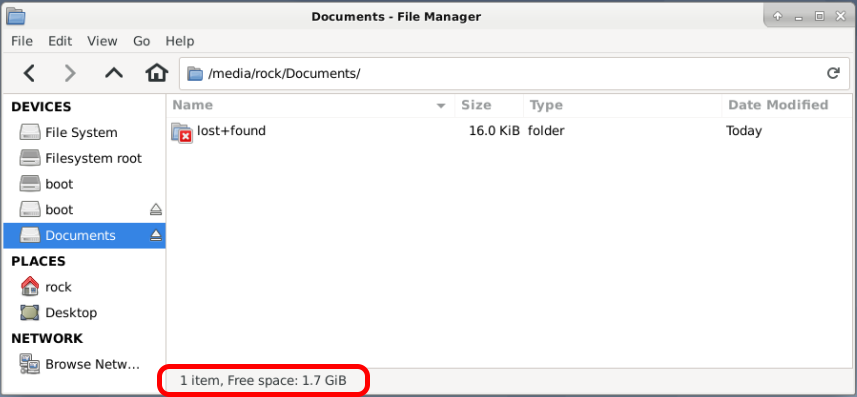
\includegraphics[width=1\textwidth]{figuren/FileManagerUsbStick}
		\caption{File Manager}
		\label{fig:FileManagerUsbStick}   
	\end{center}
\end{figure}

Met de 'File Manager' kun je in het bestandssysteem van Linux kijken.\newline
Bij het practicum begin je altijd in de home directory van gebruiker \textbf{rock} (\texttt{/home/rock}). Je werkt \textit{uitsluitend} in de map Documents (\texttt{/home/rock/Documents}).\newline
Als je meer wilt weten over het Linux bestandssysteem, \href{https://www.techrepublic.com/article/linux-101-demystifying-the-linux-directory-structure/}{klik dan hier}.

	\chapter{Klasse en objecten in C++}
Als eerste wordt er verbinding gemaakt vanaf je laptop met de RockPi, waarna een LEDje aan- en uitgezet wordt. Vervolgens wordt door middel van een programma een aantal LEDs aangestuurd.

\begin{comment}
Het practicum wordt gedaan op een RockPi dit is een single board computer dat draait in ons geval met het linux operating systeem. Met behulp van de RockPi wordt tijdens het practicum door middel van objecten diverse LEDs aangestuurd. Dit wordt gedaan door een 1 of een 0 naar naar een file te schrijven. In Figuur \ref{fig:netw} wordt weergegeven hoe de RockPi op het lab netwerk is aangesloten.
\begin{figure}[h!]
	\centering
	\begin{center} 	
			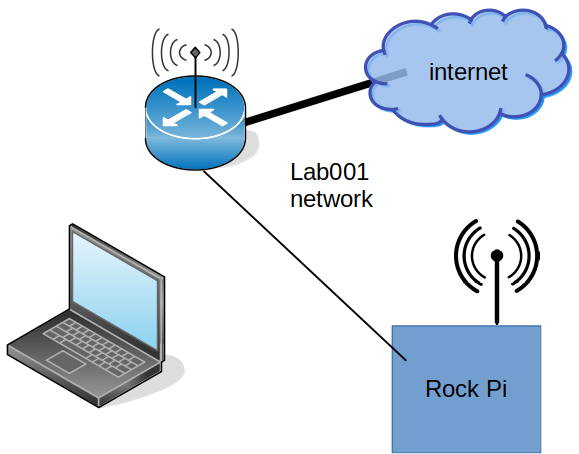
\includegraphics[width=0.4\textwidth]{figuren/laBnetwork}
			\caption{De rockPi in het lab-netwerk}
      	\label{fig:netw}   
	\end{center}
\end{figure}
Dit kan via de lab-wifi of via een UTP kabel. Het bijbehorende Ipnr. wordt getoond op het 
displaytje dat aangesloten is op de RockPi. Om contact te kunnen maken tussen de laptop en de RockPi moet de laptop \textbf{ook} op het \textbf{labnetwerk(Lab001) aangesloten} zijn, b.v. via de wifi.


\section{De eerste kennismaking met de RockPi.}

\end{comment}

\section{Werken met de RockPi.}

\subsection{Verbinding opzetten met de RockPi}\label{chp:contactPi}

In eerste instantie wordt er verbinding gemaakt met de RockPi via het \textit{ssh} commando.
\begin{figure}[h!]
	\centering
	\begin{center} 	
		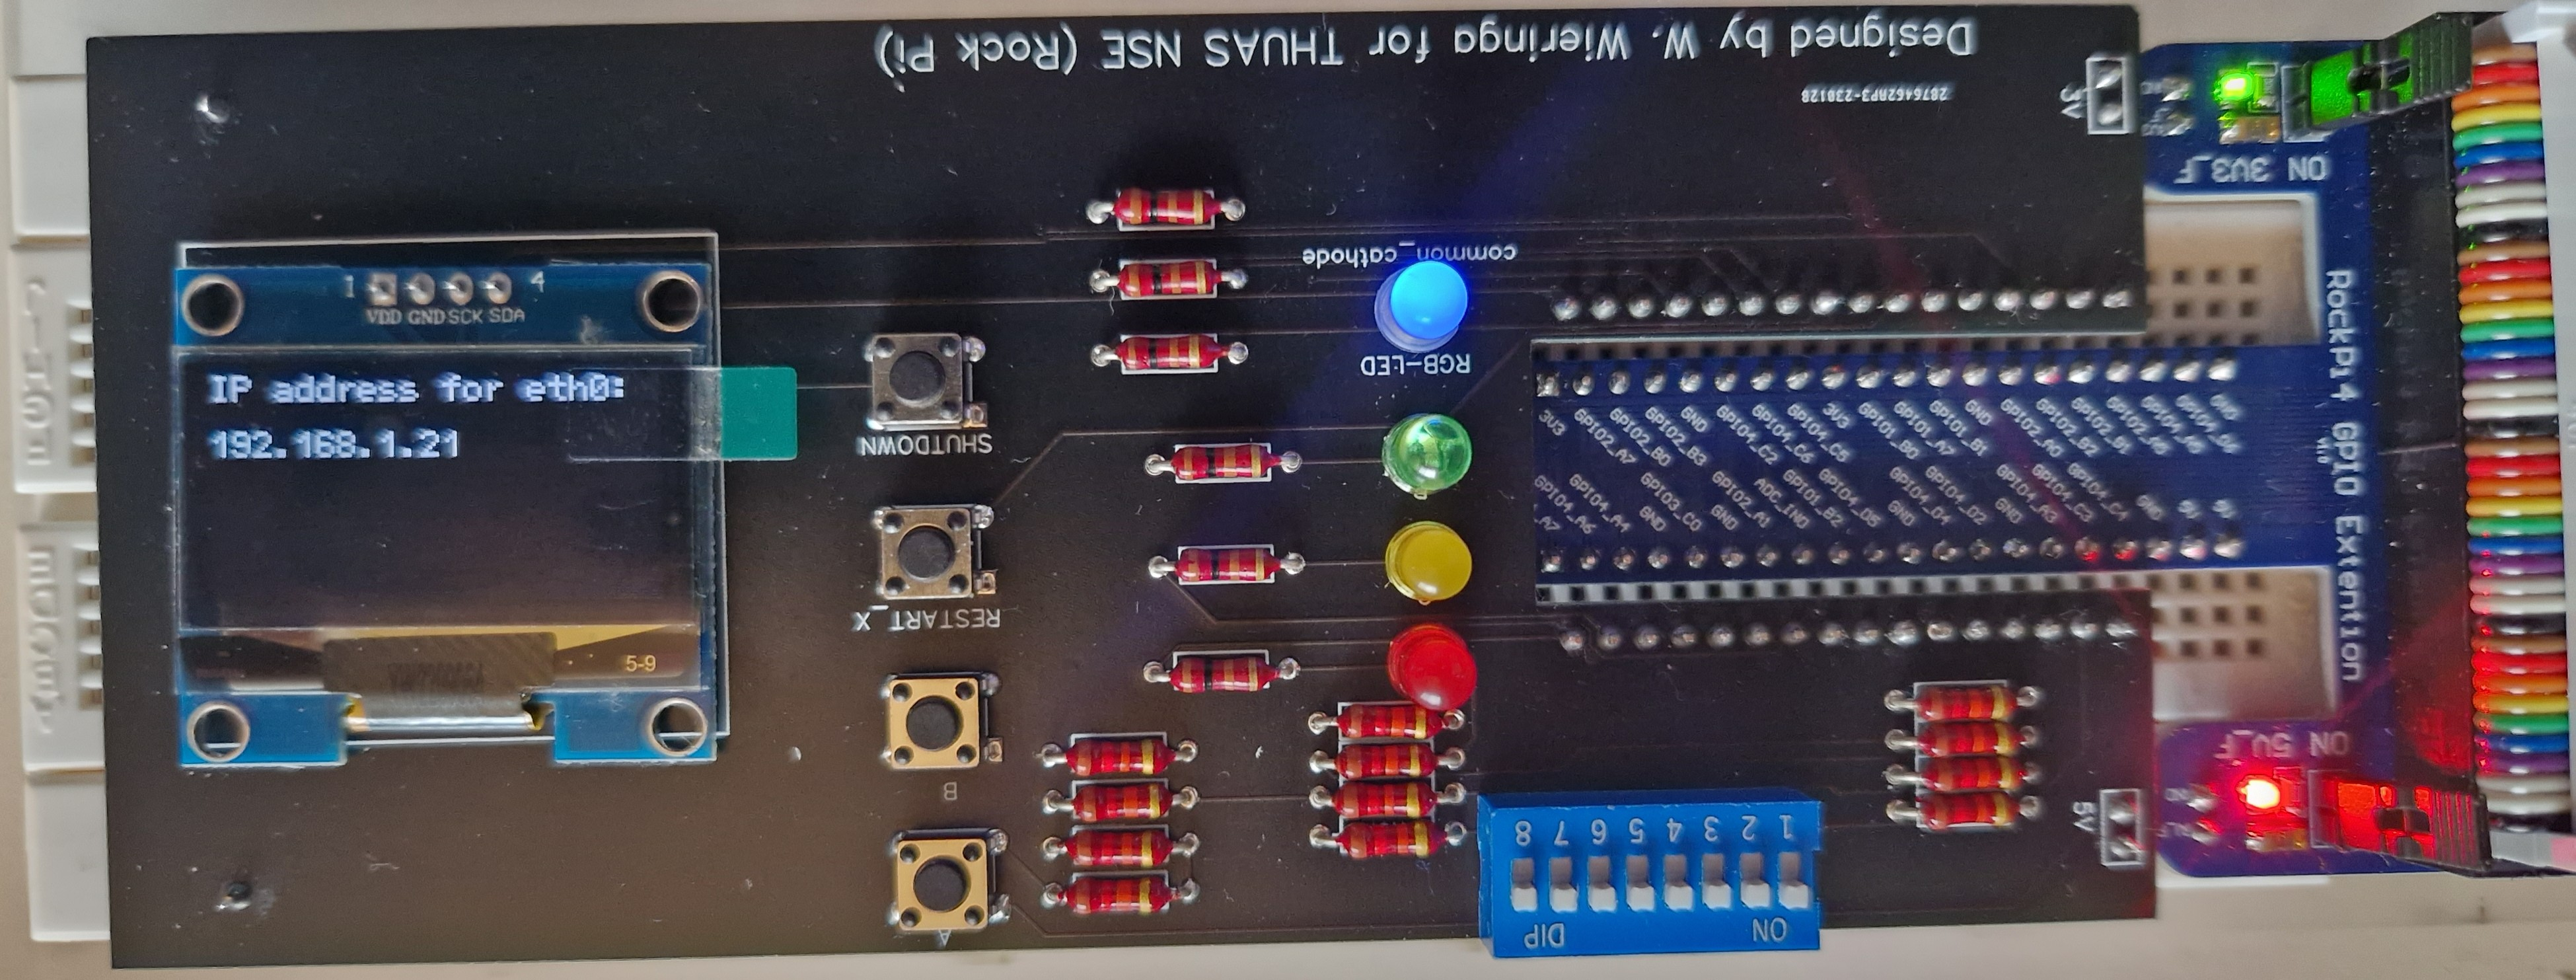
\includegraphics[width=1\textwidth]{figuren/rockIPnr}
		\caption{De RockPi met het \textit{IP adres.}}
		\label{fig:rockpiip}   
	\end{center}
\end{figure}
 Het IP adres van de RockPi is af te lezen via het oled display zoals in Figuur \ref{fig:rockpiip} wordt weergegeven. In het voorbeeld hierna wordt het IP adres \textit{192.168.178.89} gebruikt.


Open in Windows een terminal (b.v. een PowerShell, cmd prompt of een extern programma zoals b.v. \href{https://www.fosshub.com/KiTTY.html}{KiTTY}). We gebruiken voor nu PowerShell: Ga naar Windows Search: druk Windows+S (de knop met het Windows vlaggetje + de 'S'), zie Figuur \ref{fig:windowsZk} en
\begin{figure}[h!]
	\centering
	\begin{center} 	
		%\begin{subfigure}[b]{0.63\textwidth}
			
\includegraphics[width=1\textwidth]{figuren/windowsPowerShellSearch}
			\caption{Zoekscherm in Windows}
			\label{fig:windowsZk}
		%\end{subfigure}
	\begin{comment}
		\begin{subfigure}[b]{0.63\textwidth}
			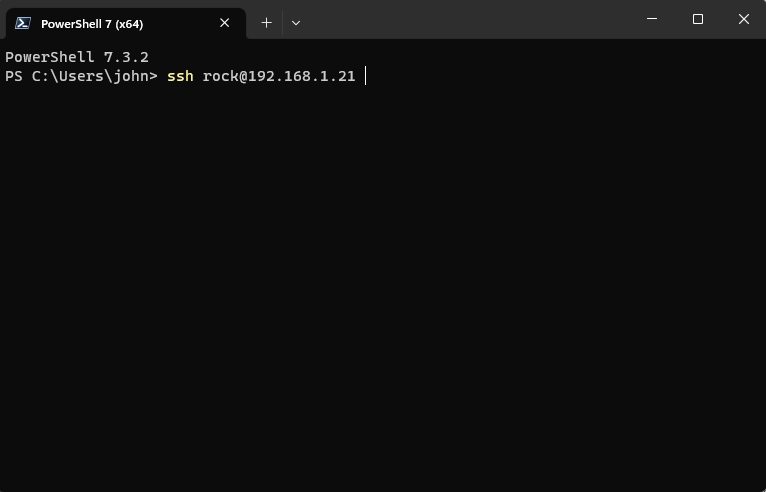
\includegraphics[width=1\textwidth]{figuren/powershell}
			\caption{ssh verbinding maken naar de RockPi }
			\label{fig:sshPi}
		\end{subfigure}
		\caption{Opstelling bij opdracht 1.}
		\label{fig:contactPi}   
	\end{comment}
	\end{center}
\end{figure}
tik vervolgens in: \textit{powershell}. In de PowerShell kan het \textit{ssh} commando met de username en het IP adres gegeven worden, zoals in figuur \ref{fig:rockpiLogIn} wordt weergegeven. Bij de eerste keer zal de melding komen of de host key moet worden opgeslagen, kies \textit{yes}. Vervolgens zal om om het password gevraagd worden. Dit is \textit{rock}. 

\clearpage
Wanneer het inloggen gelukt is, verschijnt een verhaaltje dat eindigt met de prompt van de RockPi, zoals in figuur \ref{fig:rockpiLogIn} te zien is.
\begin{figure}[h!]
	\centering
	\begin{center} 	
		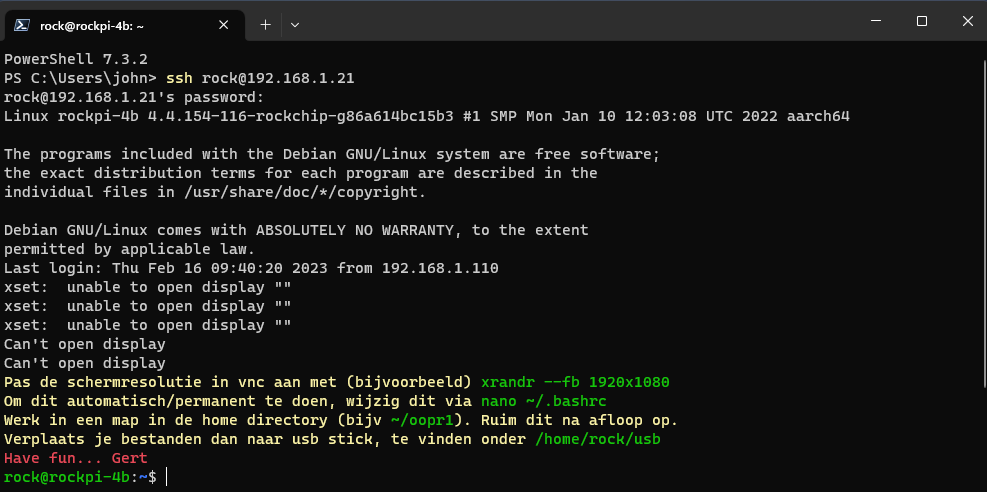
\includegraphics[width=1\textwidth]{figuren/ingelogtRockPi}
		\caption{Ingelogd in de RockPi}
		\label{fig:rockpiLogIn}   
	\end{center}
\end{figure}
Vanaf nu werk je in een Linux terminal omgeving. Een listing van een directory kan opgevraagd worden met het \textit{ls} commando, het veranderen van een directory kan gedaan worden het \textit{cd} commando (change directory) en het maken van een directory met het \textit{mkdir}  commando (make directory). Verdere Linux commando's en tips zijn te vinden in  \hyperlink{LinuxTipsTrics}{de Bijlage}.

\clearpage
\subsection{Het aansturen van een LED.}
Wanneer contact is gemaakt met de RockPi, zoals beschreven in hoofdstuk \ref{chp:contactPi}, kunnen de LEDs aangestuurd worden. De LED's zitten aangesloten op de GPIO ('General Purpose Input Output') connector van de RockPI, deze is te zien in Figuur \ref{fig:rockpiCon}.
\begin{figure}[h!]
	\centering
	\begin{center} 	
		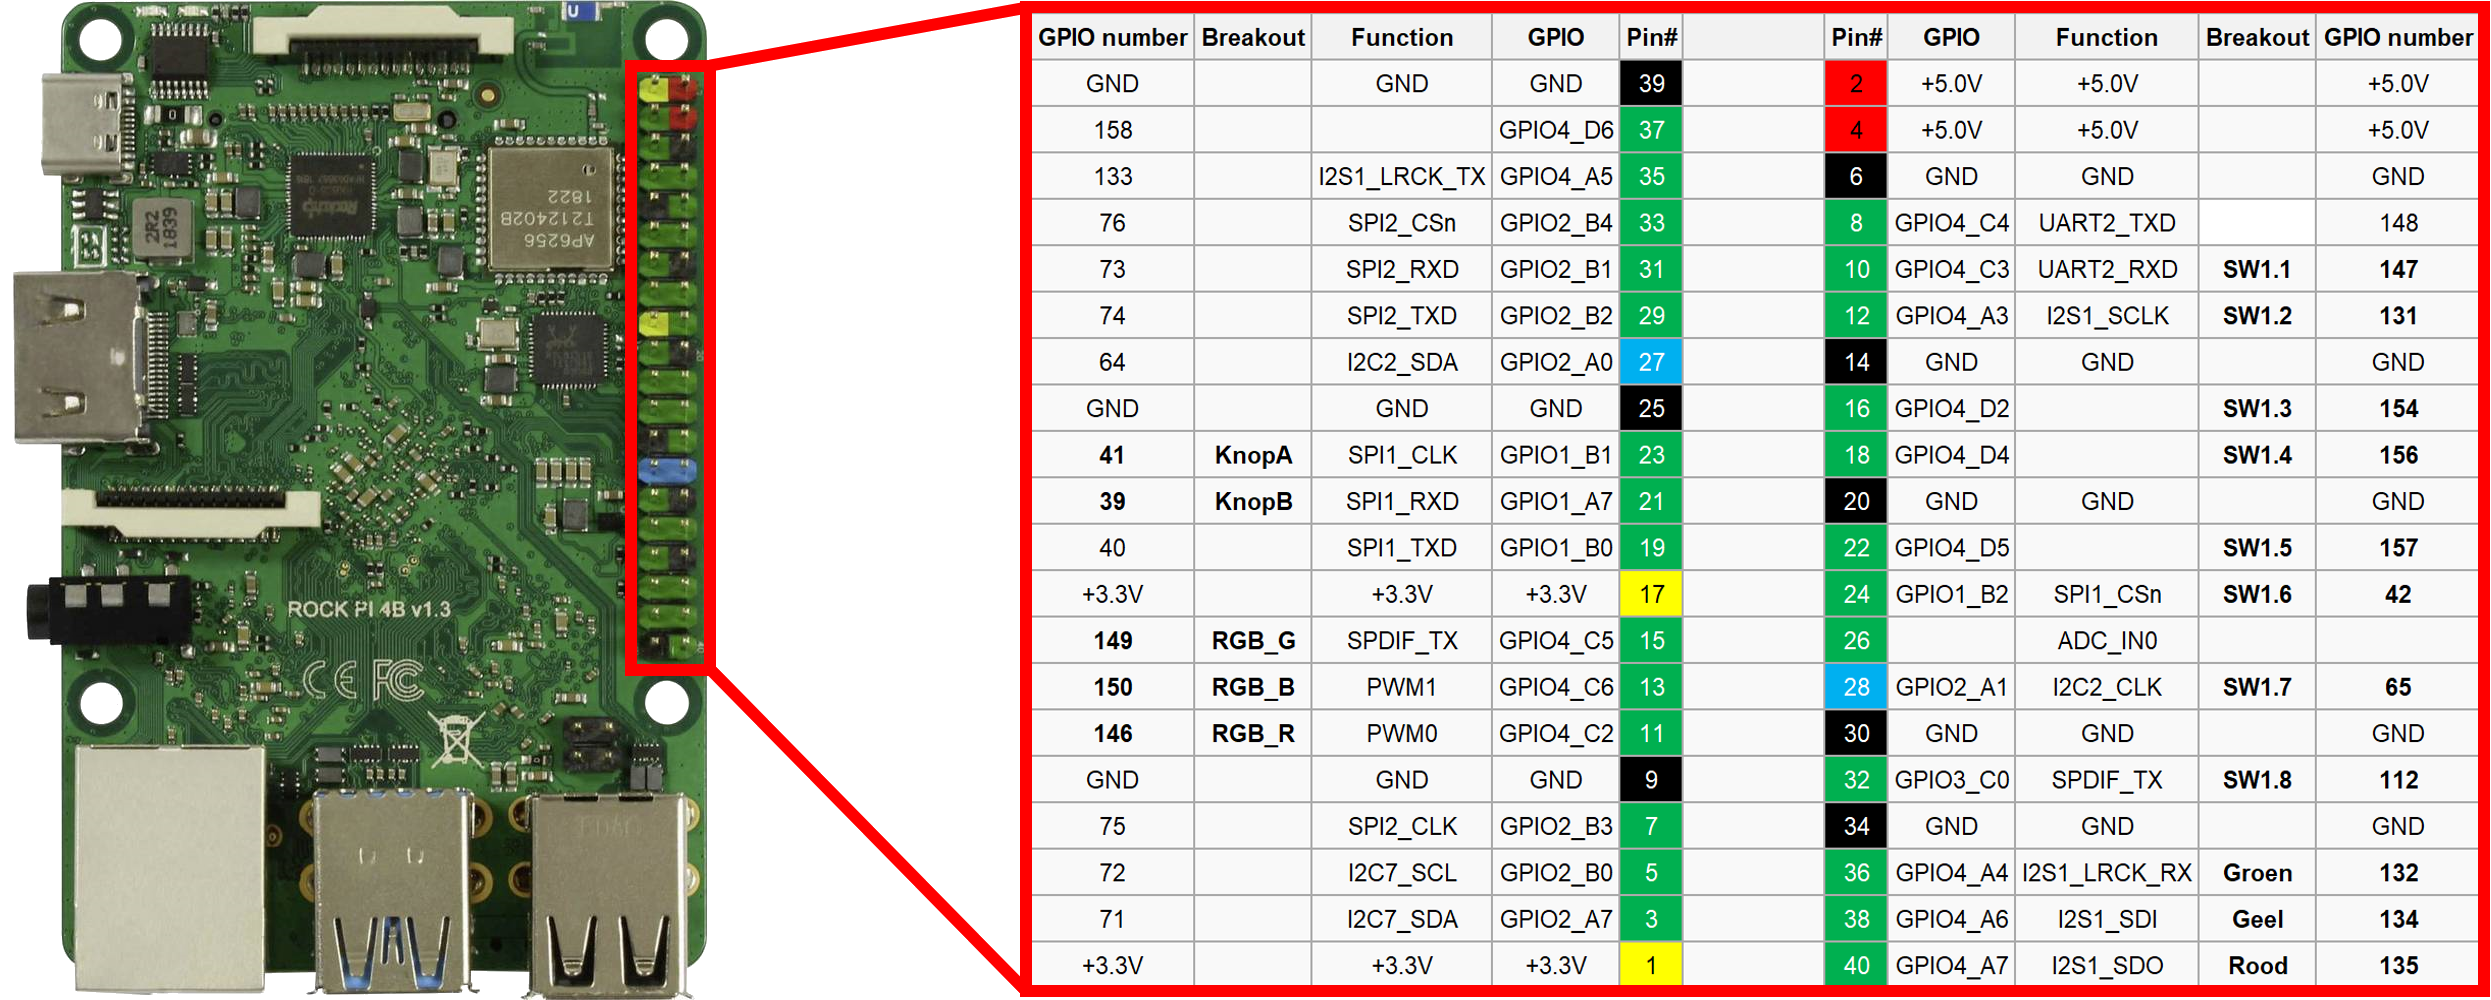
\includegraphics[width=1.1\textwidth]{figuren/rockpi-connector}
		\caption{GPIO connector van de RockPI}
		\label{fig:rockpiCon}   
	\end{center}
\end{figure}
De buitenste kolom geeft het GPIO nummer aan waarop deze geprogrammeerd kan worden. Zo zit de rode LED aangesloten op GPIO nummer 135. De \textbf{dikgedrukte} pinnen worden gebruikt met de printplaat. In de kolom \textbf{breakout} zie je wat op die pinnen zit.

\paragraph[Opdracht 1a]{Opdracht 1a, het eerste programmaatje op de RockPI}	

\begin{enumerate}
	\item Plaats de \hyperlink{chp:USBstick}{USB stick} in de RockPi.
	\item Ga naar de directory van je USB stick
	\begin{itemize}
		\item \textit{cd Documents} (het hele pad is \textit{/media/rock/Documents} )
	\end{itemize}
    
    \item Maak een directory \textit{ledje} aan en ga daar na toe.
	\begin{itemize}
	    \item \textit{mkdir ledje}
	    \item \textit{cd ledje}
    \end{itemize}  
   \item Download files \textit{gpiofuncties.h}, \textit{gpiofuncties.cpp}, \textit{test.cpp} van Github. Het main programma (\textit{test.cpp}) wordt in Listing \ref{lst:mainLd} weergegeven
   	\begin{itemize}
     	\item \textit{git clone https://github.com/JohnVi-hhs/oop.git}
     	\item \textit{cd oop}
     	\item \textit{ls -l}
     	\item \textit{nano test.cpp} Druk Ctrl+X om nano weer te sluiten.
   \end{itemize}

\clearpage
\begin{figure}[h!]
	\centering
	\begin{center} 	
		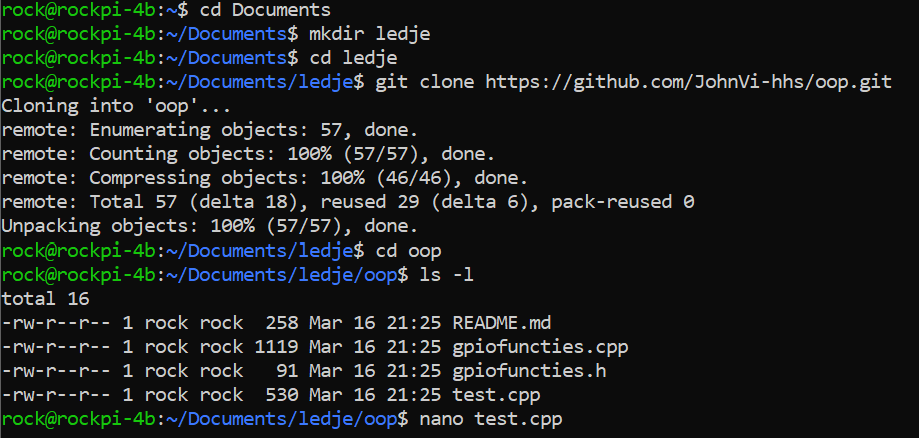
\includegraphics[width=0.94\textwidth]{figuren/gitclone}
		\caption{Schermuitvoer na bovenstaande opdrachten}
		\label{fig:gitclone}   
	\end{center}
\end{figure}

\begin{lstlisting}[caption=Zet LED aan en uit,frame=tlrb,label={lst:mainLd}]{Name}
#include <unistd.h>
#include <iostream>
#include "gpiofuncties.h"
	
using namespace std;
#define RODELED 135
	
int main() {
		
	cout<<"Hi NSE"<<endl;
	int b=zetPinOpOutput(RODELED);//return waarde of het gelukt is.
	if(b == 0)  {  //if(!b) mag ook. 
		cout<<"Foutje bedankt"<<endl;
		return 0;
	}
	cout<<"b= "<<b<<endl;//return waarde of het gelukt is.
	b=zetPinWaarde(RODELED,1);  //Zet de rode LED aan.
	usleep(1000000);
	b=zetPinWaarde(RODELED,0);  //Zet de rode LED uit.
	cout<<"einde"<<endl;
}
\end{lstlisting}
   \item Compileer en run het testprogramma.
\begin{itemize}
	\item Compileren van het programma. \\\textit{g++ -g3 *.cpp -o tst}\\
	optie \textit{-g3} heeft te maken met debug mogelijkheden. \\
	Optie \textit{-o} geeft een naam aan de output file (\textit{tst})
	\item Voer het zojuist gecompileerde programma tst uit.\\\textit{./tst}  
	
\end{itemize}
Resultaat:\\	
De rode LED gaat 1 seconde aan.

\item Pas het programma zodanig aan, zodat eerst de groene LED aangaat, daarna de gele LED en vervolgens de rode LED. \\
In de linux terminal, kunnen verschillende editors gebruikt worden, waarvan \href{https://linuxize.com/post/how-to-use-nano-text-editor/}{nano} \'{e}\'{e}n van de meest gebruikte is, een ander beroemde/beruchte editor is \href{https://opensource.com/article/19/3/getting-started-vim}{vim}  
Als je nano gebruikt: druk Ctrl+O om op te slaan en Ctrl+X om af te sluiten. Bij vim, druk/tik \textit{:help}
\end{enumerate}

\section{Het werken vanuit Visual Studio Code}

Hierbij wordt vanuit 'Visual Studio Code' (VSC) gewerkt, en wordt de klasse Led geïmplementeerd. Er wordt vanuit gegaan dat VSC geïnstalleerd is zoals in appendix  \ref{app:vsc} beschreven staat.  
\begin{enumerate}
	\item Start VSC op en maak verbinding met de RockPi.
	\begin{itemize}
		\item Klik op remote Explorer \img{figuren/remoteExplorer}. De IP nummers van de remote system(en) die al eerder gebruikt zijn worden zichtbaar, zoals te zien is in Figuur \ref{fig:remNr}
		\begin{figure}[h!]
			\centering
			\begin{center} 	
				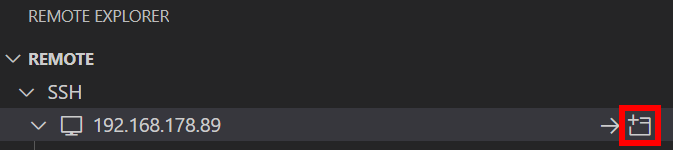
\includegraphics[width=0.5\textwidth]{figuren/remoteExplorer2}
				\caption{Remote Explorer van VSC}
				\label{fig:remNr}   
			\end{center}
		\end{figure}
				 
		\item  Maak een nieuwe connectie aan, door op \img{figuren/connectIcon} te klikken (rood omkaderd).

      \end{itemize}
      
      \item Nadat een verbinding gemaakt is met de RockPi, open een remote folder door op \img{figuren/VSCiconeExpl} te klikken (of druk Ctrl+K Ctrl+O) en ga naar de directory van de vorige opdracht: \texttt{/home/rock/Documents/ledje/oop/} \newline
      Aan de linkerkant worden de files zichtbaar en onderaan een statusbalk met informatie. Dit is te zien in figuur \ref{fig:vncOp}
  		\begin{figure}[h!]
  	\centering
  	\begin{center} 	
  		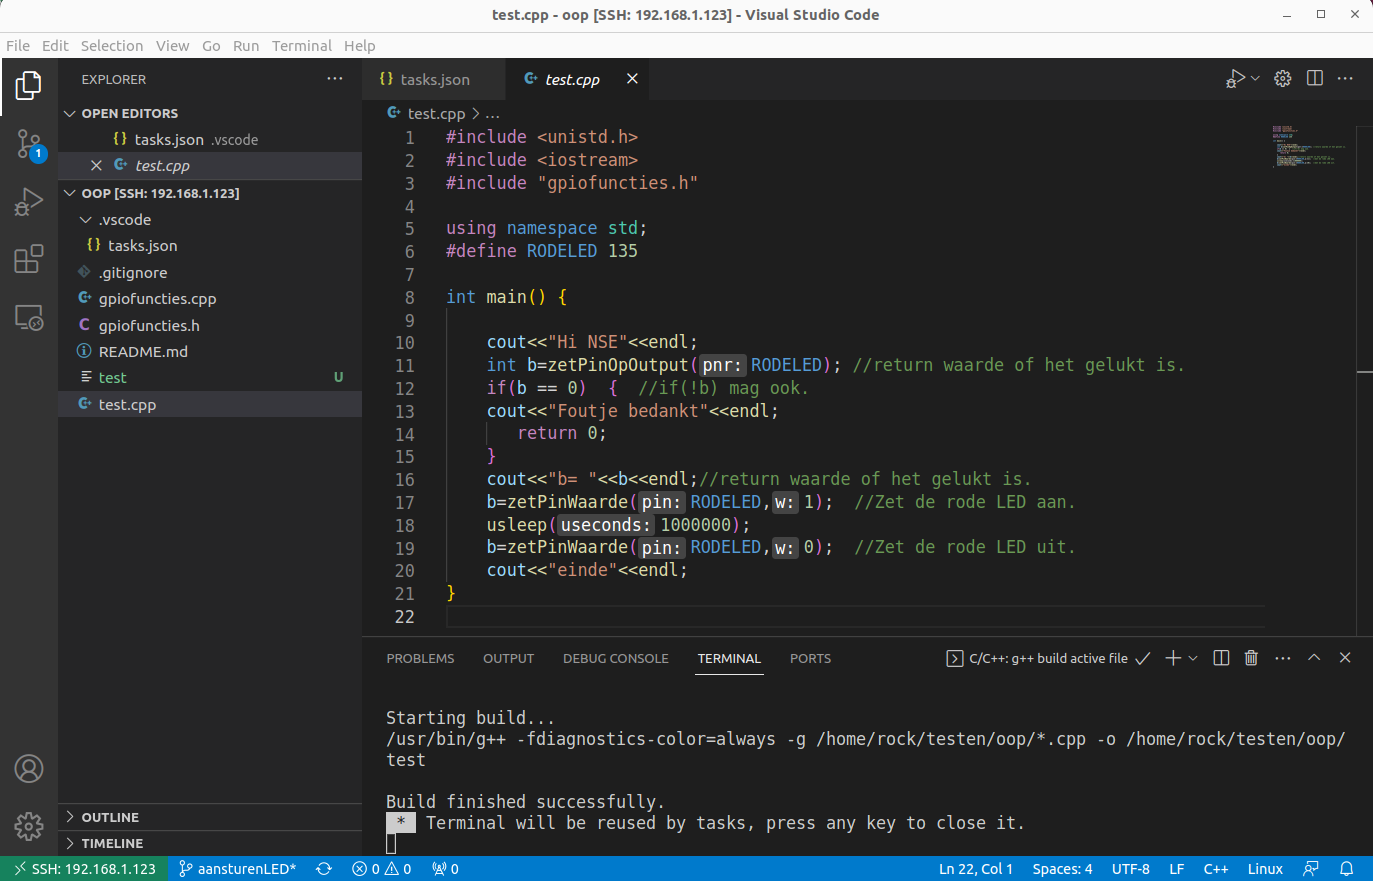
\includegraphics[width=0.72\textwidth]{figuren/vncSchermOp1}
  		\caption{VSCode in de gewenste directory}
  		\label{fig:vncOp}   
  	\end{center}
  \end{figure}    

\newpage
Klik op select folder  % Gert: Ik kan niks vinden wat 'select folder' heet
en selecteer de folder waarin de files staan. 


\begin{itemize}
	\item Selecteer de file \textit{test.cpp} en compileer de files\footnote{compileren lukt niet, controleer of C++ extension (\img{figuren/cPlusIcon} ) is geïnstalleerd} (Terminal $\rightarrow$ Run Build Task... of Ctrl+Shift+B) 
	\item Klik links van regelnummer 10, er verschijnt een rode stip, dit is een breakpoint.
	\item Selecteer bij het pijltje rechtsboven \img{figuren/debugPijl} de Debug optie en klik op de pijl (of Run $\rightarrow$ Start Debugging), de debugger wordt gestart en het  beeldscherm zoals in figuur \ref{fig:debugScherm} verschijnt.
	\begin{figure}[h!]
		\centering
		\begin{center} 	
			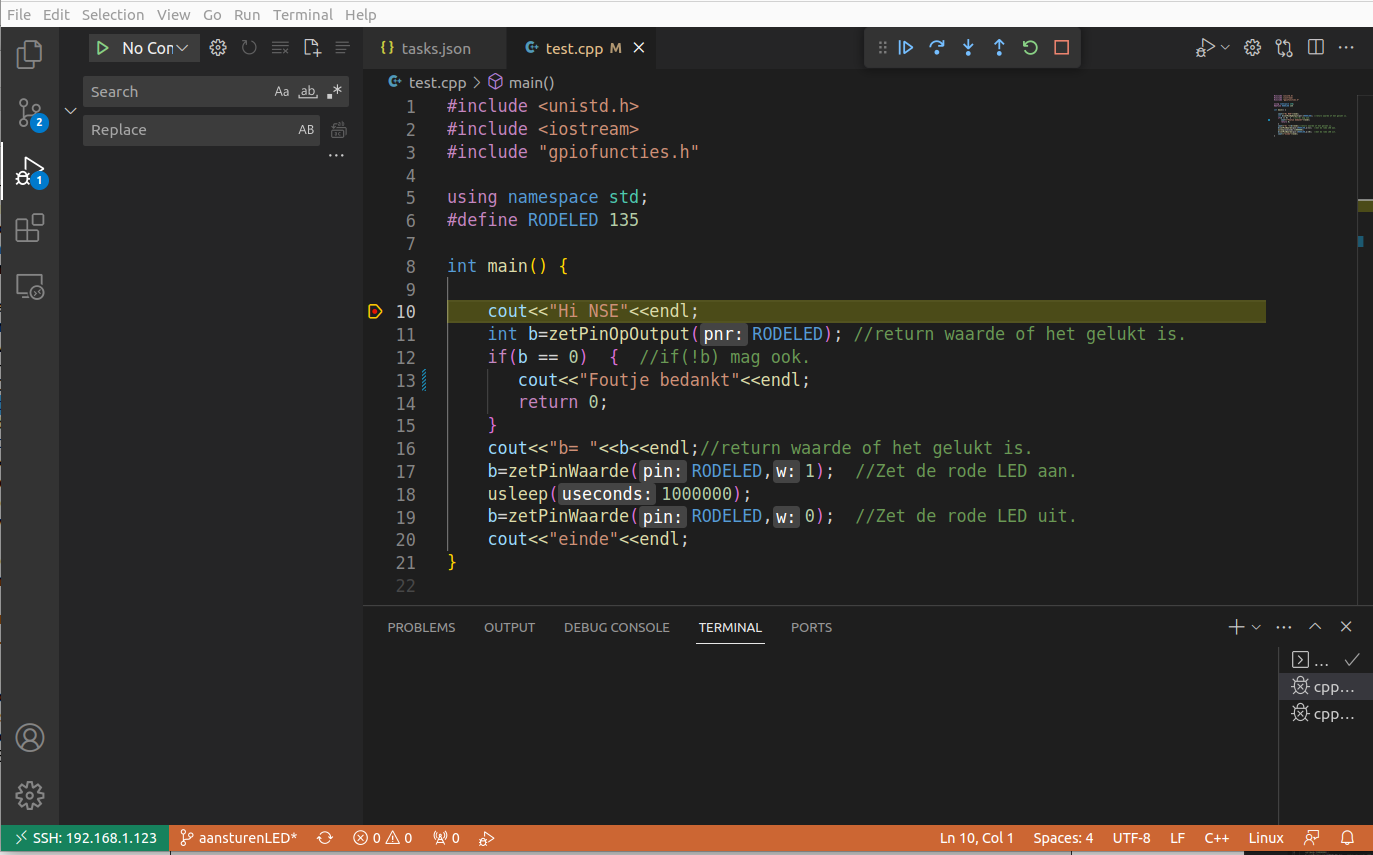
\includegraphics[width=0.9\textwidth]{figuren/debugScherm}
			\caption{Start van de debug sessie.}
			\label{fig:debugScherm}   
		\end{center}
	\end{figure}
	
	Met de debugknoppen rechtsboven kan nu stap voor stap door het programma gelopen worden.\\
	Doorloop het programma stap voor stap, zodat de LED ook daadwerkelijk bij een stap aan- en uitgaat. 
\end{itemize}

\item Bij deze opdracht wordt de eerste klasse gemaakt.
\begin{itemize}
	\item Maak een nieuwe terminal aan (Terminal $\rightarrow$ New Terminal) of Ctrl+Shift+` en maak een nieuwe directory aan.
	\item clone de volgende code:\\
	 git clone \verb|--|branch opdrLedH https://github.com/JohnVi-hhs/oop.git
	\item De UML notatie van de klasse \textbf{Led} wordt weergegeven in figuur \ref{fig:klassLed} en de headerfile in listing \ref{lst:ledH}

	\begin{minipage}{0.5\textwidth} 
	\begin{figure}[H]
	%	\caption{\label{fig:label} Figure title}
		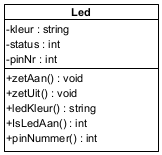
\includegraphics[width=0.9\textwidth]{figuren/klasseLedOpg1}
		\caption{UML diagram van de \\klasse Led}
		\label{fig:klassLed}   
	\end{figure}
\end{minipage}\hfill
\begin{minipage}{.45\textwidth}
	
	\begin{lstlisting}[caption=LED declaratie file(.h),frame=tlrb,label={lst:ledH}]{Name}
class Led
{
	public:
    	Led(int);
		Led(int, string);
		Led(int, string,string);
		~Led();
		void zetAan();
		void zetUit();
		string ledKleur()const;
		int isLedAan()const;
		int pinNummer() const;
		string deEigenaar() const;
			
	private:
		string kleur;
		int pinNr;
		int status;  
		string eigenaar;
};
		
		
	\end{lstlisting}
	
\end{minipage}
\paragraph{Opdracht:} Implementeer de Led.cpp zodat het hoofdprogramma van listing \ref{lst:hfdprg2} zonder errors en warning gecompileerd en uitgevoerd kan worden. 
\begin{lstlisting}[caption=Hoofdprogramma om de LED uit te testen ,frame=tlrb, label={lst:hfdprg2}]{Name}
#include <unistd.h>
#include <iostream>
#include <string>
#include "Led.h"

using namespace std;
#define RODELED 135
#define GROENELED 132
#define GELELED 134

int main() {
	
	cout<<"Hi NSE"<<endl;
	Led rood(RODELED,"Rood","Pietje Puk");
	Led geel(GELELED,"Geel");
	Led groen(GROENELED);
	
	groen.zetAan();
	usleep(1000000);
	groen.zetUit();
	geel.zetAan();
	usleep(1000000);
	geel.zetUit();
	rood.zetAan();
	usleep(1000000);  
	rood.zetUit();
	
	cout<<"einde"<<endl;
}


\end{lstlisting}	
\end{itemize}


    \end{enumerate}


\section{Het werken met een visuele debugger.}
 
Bij dit onderdeel van de opdracht wordt gewerkt met een grafische debugger. Hiermee wordt een grafische weergave gedaan wat een object is en wat een object van een afgeleide klasse inhoud (dit laatste komt in opgave 2 te spraken). Verder worden de associaties tussen objecten duidelijk weergegeven (dit wordt in week 4 en 5 gedaan).

De grafische debugger die gebruikt wordt is de DDD debugger(Data Display Debugger) 


Een paar handige links hierbij zijn:

\begin{itemize}
	\item DDD manual in \href{https://www.gnu.org/software/ddd/manual/html_mono/ddd.html}{html} en \href{https://www.gnu.org/software/ddd/manual/pdf/ddd.pdf}{pdf}
	\item \href{https://www.gnu.org/software/ddd/}{GNU DDD project}
	\item \href{href="https://taufanlubis.wordpress.com/2019/02/19/gnu-debugger-front-end-graphical-user-interface-with-ddd}{taufanlubis.wordpress.com}
	\item  \href{https://www.cs.swarthmore.edu/~newhall/unixhelp/howto_gdb.php}{Swarthmore}
	\item  \href{http://www.linuxfocus.org/English/January1998/article20.html}{linuxfocus}
\end{itemize}

De instellingen van de DDD debugger staan in de file .ddd die staat in de home directory (\textit{/home/rock}). Soms is het eenvoudiger om deze directory te deleten dan de instellingen aan te passen.

We gaan nu met de DDD debugger werken.
Om met DDD te kunnen werken hebben we een grafische omgeving nodig. Een handige methode is om de de VNC viewer van de host te gebruiken. Deze viewer toont de grafische uitvoer van de RockPi. Open in de VNC een terminal, ga naar de directory die in de vorige opdracht gemaakt is (waar de files test.cpp, Led.cpp en Led.h \textcolor{green}{test} staan) en start de DDD debugger op:
\texttt{\textit{ddd test}}, vervolgens wordt het scherm, zoals weergegeven in Figuur \ref{fig:dddscherm1}, getoond.
\begin{figure}[h!]
	\captionsetup{justification=centering}
	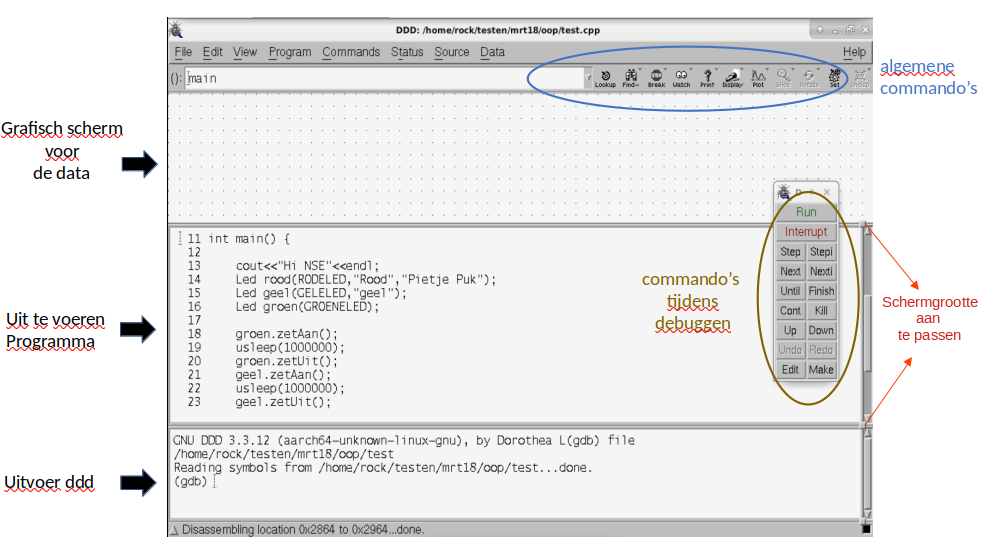
\includegraphics[width=0.8 \linewidth]{figuren/ddd_startup_screen}
	\centering
	\caption{het DDD opstartscherm.}
	\label{fig:dddscherm1}
\end{figure}

\paragraph{Opdracht}
We gaan hierbij stap voor stap het programma doorlopen, waarbij de inhoud van de objecten van de klasse Led wordt getoond.

\begin{enumerate} [label=\alph*]
	\item Als eerste een korte kennismaking met de DDD debugger.
\begin{enumerate} [label=\roman*]

	\item Ga met de cursor op de regel \texttt{\textit{ Led rood(RODELED,"Rood", "Pietje Puk");}}
	(regelnummer 14)
	\item Klik op \textit{Break} (bij algemene commando's). Voor het begin van de regel verschijnt nu een breakpoint.

\begin{figure}[h!]
	\captionsetup{justification=centering}
	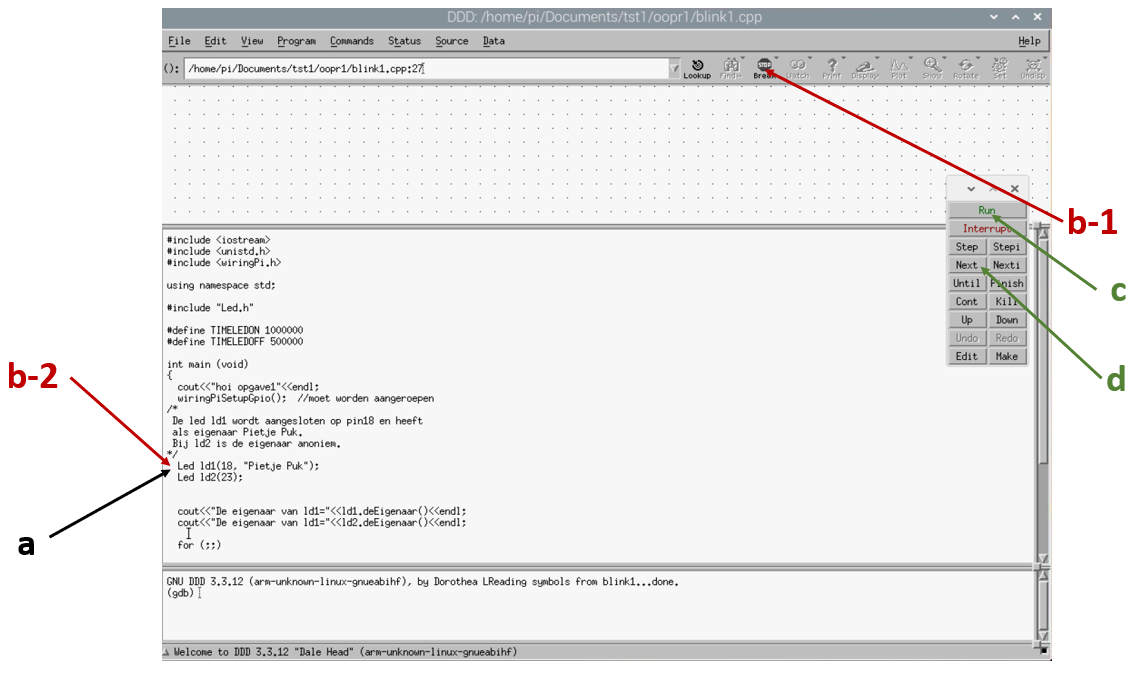
\includegraphics[width=0.7 \linewidth]{figuren/ddd_set_breakpoint}
	\centering
	\caption{het zetten van een breakpoint.}
	\label{fig:ddduitv1}
\end{figure}
	\item Klik op \textit{Run} (bij debug commando's),
het programma wordt uitgevoerd tot het breakpoint. Er verschijn een groene pijl bij het breakpoint.
\item Klik op \textit{Next}, de regel wordt uitgevoerd. \\
De groene pijl komt voor de regel \textit{Led geel(GELELED,"Geel");} te staan. 
\item Klik op step, met dit commando \textit{Step} wordt in de constructor van de klasse Led gestapt. Doorloop het programma verder stap voor stap.

\end{enumerate}
\item Het zichtbaar maken van de inhoud van de objecten.


\begin{enumerate} [label=\roman*]
	\item Start de DDD debugger op (\texttt{\textit{ddd test}}):
		\item Zet een breakpoint op de regel	\textit{groen.zetAan();} 
		\item Klik met de muis op variabele \texttt{rood} en vervolgens op Display of klik met rechtermuisknop en vervolgens op Display rood. Het object \texttt{rood} van de Klasse Led wordt nu weergegeven.
		\item Doe hetzelfde met de variabele \texttt{geel} en \texttt{groen}.
		\item Als het goed is ziet de debugger er ongeveer uit zoals Figuur \ref{fig:dddLeds}, alleen met je \textcolor{BrickRed}{eigen naam}.  
	    \item Ga met het Step commando de methode \texttt{zetAan} van groen in.
		\item Ga met het Step commando de methode \texttt{zetAan} van geel in. Je ziet dat de methode hetzelfde is, alleen de attributen hebben een andere waarde.
		  \begin{figure}[h!]
		 	\captionsetup{justification=centering}
		 	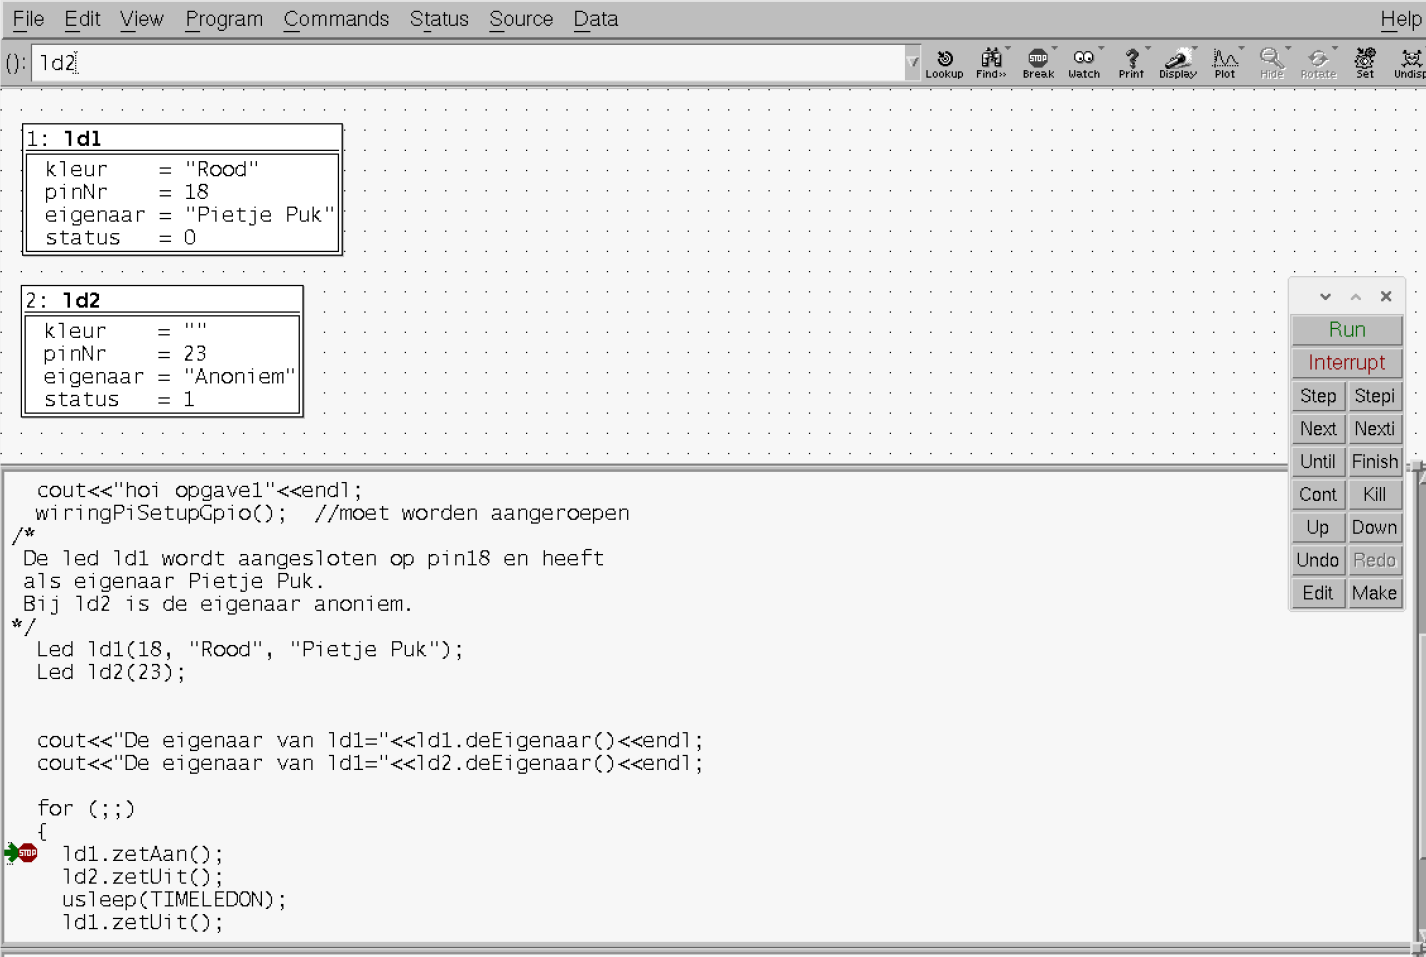
\includegraphics[width=0.9 \linewidth]{figuren/LedDDD}
		 	\centering
		 	\caption{Weergave van twee objecten van de klasse Led.}
		 	\label{fig:dddLeds}
		 \end{figure}
\end{enumerate}
	 \item Maak een screenshot die lijkt op Figuur \ref{fig:dddLeds} alleen met je \textbf{eigen naam} in plaats van ''Pietje Puk'' en upload deze op Brightspace.
	 \item Laat de opdracht aftekenen met onder andere een zichtbaar screenshot.
 
\end{enumerate}


	\chapter{Afgeleide klasse en objecten in C++}

Bij deze opdracht richten we ons hoe bij OO componenten Overerving en Polymorfisme getest kunnen worden met een debugger.

Deze opdracht bestaat verder uit de deelopdrachten A en B en er moeten 6 screenshots gemaakt worden die op brightspace moeten worden geüpload. Alle deelopdrachten moet je laten aftekenen door de docent.

Er zijn diverse soorten LEDs, zoals in figuur \ref{fig:LEDs} te zien zijn. Deze zijn:
\begin{itemize}
	\item SingleLed: deze LEDs hebben 1 kleur, twee pootjes en worden aan 1 poort op de RockPi aangesloten, zoals de rode, oranje en groene LED. Een voorbeeld wordt weergegeven in figuur \ref{fig:singleLed}
	\item DualLed: deze LEDs hebben 2 mogelijke kleuren, drie pootjes en worden aan 2 poorten (1 per kleur) aan de RockPi verbonden. Een voorbeeld wordt weergegeven in figuur \ref{fig:dualLed}
	\item RGB Led: deze LEDs hebben de kleuren rood, groen en blauw in 1 behuizing en hebben vier pootjes, waarvan 3 worden aangesloten op de poorten (1 per kleur) van de RockPi.De LED met de witte kleur op het practicumboord is een RGB LED. Een voorbeeld van een RGB LED wordt weergegeven in figuur \ref{fig:rgbLed}
\end{itemize}

\begin{figure}[h!]
	\centering
	\begin{subfigure}[b]{0.3\textwidth}
		\centering
		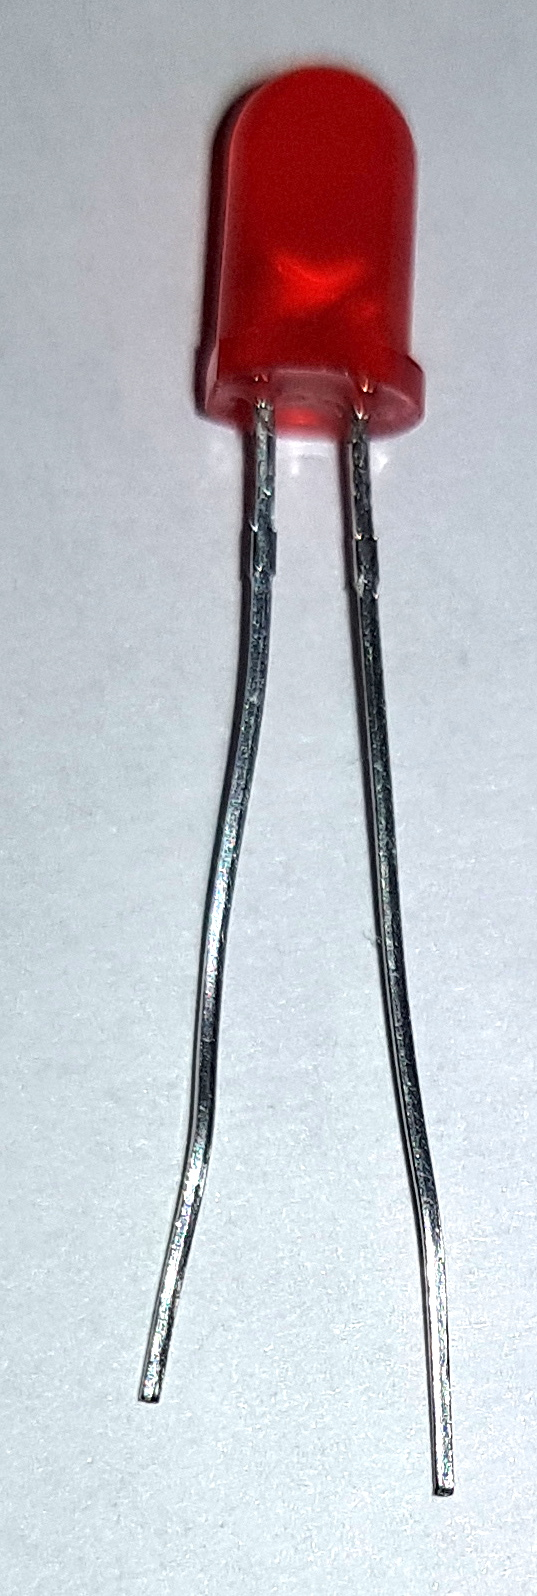
\includegraphics[width=0.7\textwidth,height=3.5cm]{figuren/singleled}
		\caption{een single LED}
		\label{fig:singleLed}
	\end{subfigure}
	\hfill
	\begin{subfigure}[b]{0.3\textwidth}
		\centering
		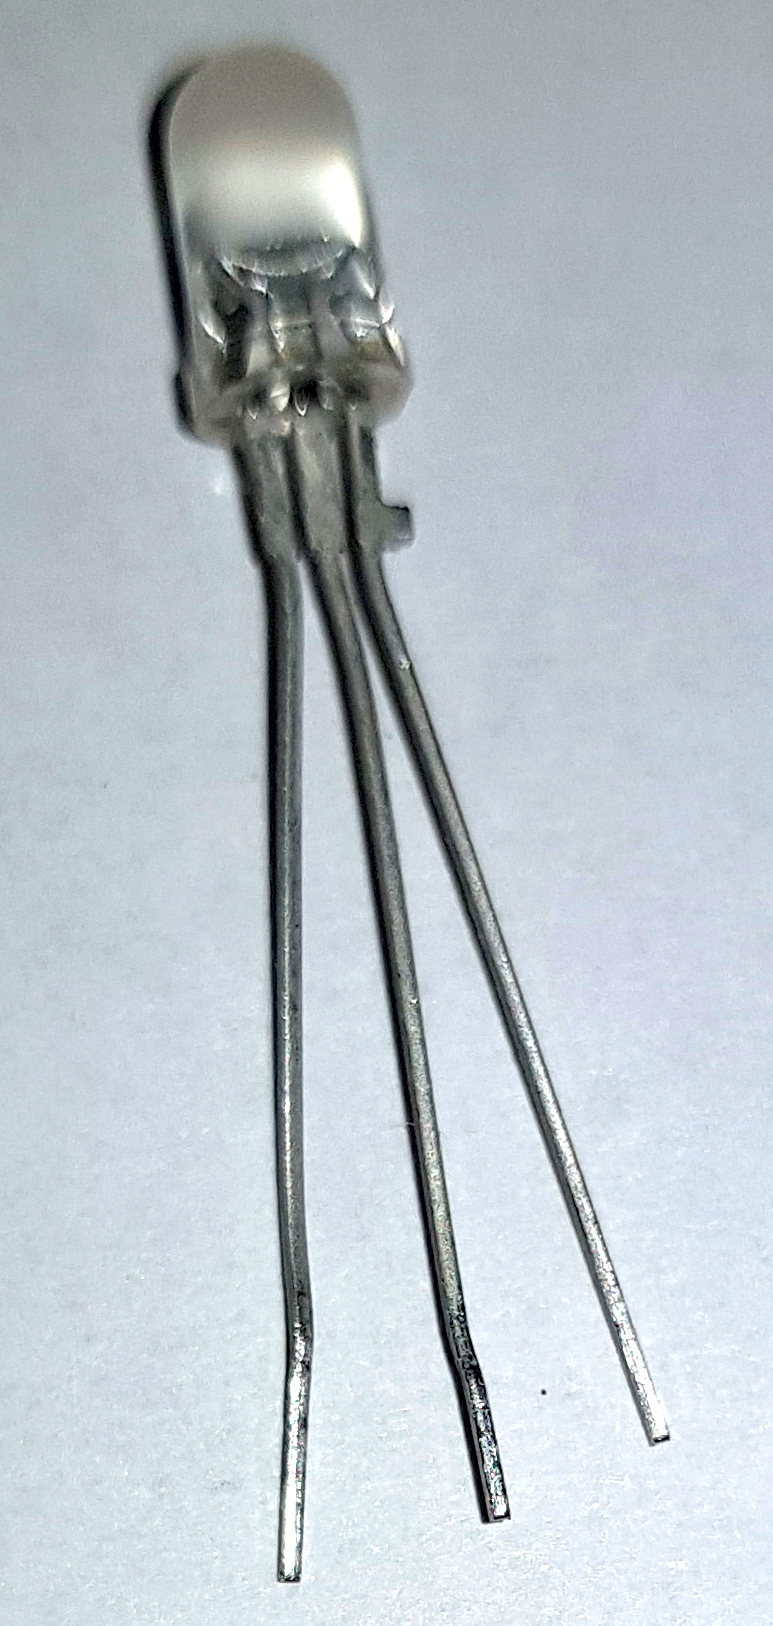
\includegraphics[width=0.7\textwidth,height=3.5cm]{figuren/dualled}
		\caption{een dual LED}
		\label{fig:dualLed}
	\end{subfigure}
	\hfill
	\begin{subfigure}[b]{0.3\textwidth}
		\centering
		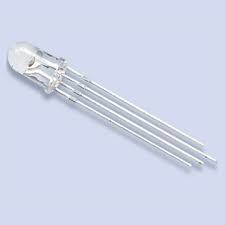
\includegraphics[width=0.9\textwidth,height=3.5cm]{figuren/rgbled}
		\caption{een RGB LED}
		\label{fig:rgbLed}
	\end{subfigure}
	\caption{Verschillende type LEDs}
	\label{fig:LEDs}
\end{figure}

De analist die de eisen voor de controller-software voor de LED controllers opstelt, heeft bedacht dat het in de toekomst mogelijk moet kunnen zijn om nieuwe LED types toe te voegen, bijvoorbeeld 3 kleuren LEDS. De controller software moet dus zo veel mogelijk onafhankelijk van het concrete LED type gemaakt worden. In figuur \ref{fig:klassLed} wordt de UML weergave geaan van zowel de SingleLed als de RGBLed
\begin{figure}[h!]
	\captionsetup{justification=centering}
	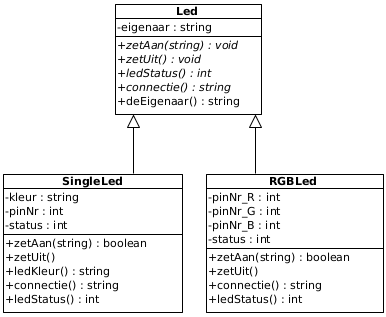
\includegraphics[width=0.6 \linewidth]{figuren/rgbKlasse}
	\centering
	\caption{De afgeleide klassen singleLed en RGBLed .}
	\label{fig:klasAfg}
\end{figure}
\newpage
De werking is als volgt.

\begin{itemize}
	\item Een LED wordt aangezet door de methode bool zetAan(string k); waarbij de parameter de kleur is die aangezet moet worden.
	\begin{itemize}
		\item Wordt bij een groene LED ''groen''  meegegeven, wordt de LED aangezet en true geretourneerd.
		\item Wordt bij een groene LED ''rood'' meegegeven, wordt de LED niet aangezet en wordt false geretourneerd.
	\end{itemize}
\item Een LED wordt uitgezet door de methode void zetUit(); Dit houd in dat bij een RGBLed alle kleuren uitgezet worden.
\item De methode string connectie(); geeft het gpioNummer van het aangesloten platform mee terug. In het geval van de RGBLed wordt een string mee teruggegeven met alle drie de gpioNummers gescheiden door een spatie.
\item Doordat de status van de LED verschillend zijn (een singleLed kan alleen aan en uit terwijl bij de RGBLed kan kleur1, kleur 2, kleur 3 of een combinatie van kleuren aan- en uitgaan), heeft elke afgeleide LED een eigen status.
	
\end{itemize}

\paragraph{Opdracht} 



	\chapter{Een compositie en aggregatie.}
\label{ch:hfstCompAgg}
Bij deze opdracht zal een aggregatie en compositie in C++ geïmplementeerd worden. Met behulp van de DDD debugger worden objecten en hun onderlinge verbindingen zichtbaar gemaakt. Hiervan zullen verschillende screenshots gemaakt moeten worden die opgenomen  moeten worden in je portfolio. De portfolio moet aan het einde van de week geüpload worden op Brightspace. Tijdens het aftekenen moeten de screenshots zichtbaar zijn.
Op de screenshots zal je \textbf{eigen} \textcolor{BrickRed}{\textbf{naam}} en \textcolor{BrickRed}{\textbf{studienummer}} moeten staan.

De opdracht bestaat uit een speciaal type LED, de LogLed. De LogLed heeft als extra een stopwatch,en een Tijdsduur. De klasse wordt weergegeven in figuur \ref{fig:logled}.
    \begin{figure}[h!]
	\captionsetup{justification=centering}
	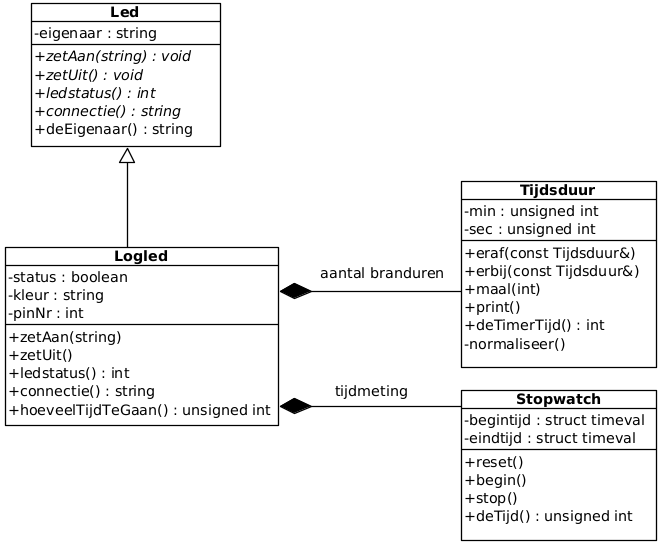
\includegraphics[width=0.9 \linewidth]{figuren/logled}      %ledPlatform}
\centering
\caption{De logled met timer en stopwatch.}
\label{fig:logled}
\end{figure} 
De logled is speciaal ontwikkelt om ervoor te zorgen dat een LED maar een maximum aan uren aan kan. daarna moet een nieuwe logled gekocht worden. 
\begin{itemize}
	\item Met het tijdsduur wordt bijgehouden hoeveel minuten de logled nog aan mag. 
	\item Met de stopwatch wordt elke keer gecheckt hoelang de logled voor dat moment aan is.
	\item De Led kan hergebruikt worden uit de vorige opgave, De stopwatch krijg je cadeau en is te downloaden van github. \\De klasse Logled en Tijdsduur moet je zelf maken.
\end{itemize}

\section{De klasse Tijdsduur.}

We willen een ADT (Abstract Data Type) , ook wel zelfgedefinieerd datatype genoemd, maken waarin een tijdsduur in minuten en seconden kan worden opgeslagen. De totale tijd in seconden kan ook worden opgevraagd. 
\begin{figure}[h!]
	\captionsetup{justification=centering}
	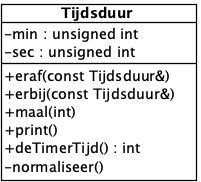
\includegraphics[width=0.28 \linewidth]{figuren/tijdsduur}
	\centering
	\caption{weergave van de klasse Tijdsduur. }
	\label{fig:tijdsduurKlas}
\end{figure}
We noemen dit zelf gedefinieerde datatype \texttt{Tijdsduur}. Figuur \ref{fig:tijdsduurKlas} geeft de klasse weer van Tijdsduur.
Het ADT \texttt{Tijdsduur} kan in C++ als volgt gedeclareerd worden in de header file (tijdsduur.h):

\begin{lstlisting}[caption= de headerfile van de klasse \texttt{Tijdsduur},label={lst:tijdsdHeader},numbers=none]		
	#ifndef TIJDSDUUR_H
	#define TIJDSDUUR_H
	
	// De declaratie van de ADT Tijdsduur:
	class Tijdsduur {
		public:
		//...
		void eraf(Tijdsduur t);
		//...
		
		private:
		int sec;
		//...
	};
	#endif // TIJDSDUUR_H
\end{lstlisting}

De implementatie (\texttt{tijdsduur.cpp}) ziet er tot nu toe als volgt uit:
\begin{lstlisting}[caption= de implementatiefile van de klasse \texttt{Tijdsduur},label={lst:tijdsdImpl},numbers=none]
	#include <iostream>
	#include "tijdsduur.h"
	#include <iomanip>
	using namespace std;
	
	// De definities van de memberfunctie van de ADT Tijdsduur, oftewel: de implementatie van de ADT Tijdsduur:
	void Tijdsduur::eraf(Tijdsduur t) {
		sec-=t.sec;
		//...
	}
\end{lstlisting}

Het hoofdprogramma (\texttt{opg13.cpp}) ziet er als volgt uit:

\begin{lstlisting}[caption= de implementatiefile van het hoofdprogramma ,label={lst:tijdsdMainprog},numbers=none]
	#include <iostream> // nodig voor cout (schrijven naar scherm)
	#include <iomanip> // nodig voor setw (veldbreedte definieren )
	#include "tijdsduur.h"
	using namespace std;
	
	int main() {
		Tijdsduur t1(3,50); // t1 is 3 minuten en 50 seconden
		cout<<"t1 = "; t1.print(); cout<<endl;
		const Tijdsduur kw(15); // kw is 15 seconden
		cout<<"kw = "; kw.print(); cout<<endl;
		t1.erbij(kw); // Tel kw bij t1 op
		cout<<"t1 = "; t1.print(); cout<<endl;
		Tijdsduur t2(t1); // t2 is een kopie van t1
		t2.eraf(kw); // Trek kw van t2 af
		cout<<"t2 = "; t2.print(); cout<<endl;
		t2.maal(7); // Vermenigvuldig t2 met 7
		cout<<"t2 = "; t2.print(); cout<<endl;
		Tijdsduur t3(3,-122); // t3 is 3 minuten minus 122 seconden
		cout<<"t3 = "; t3.print(); cout<<endl;
		t3.eraf(t2); 
		cout<<"t3 = "; t3.print(); cout<<endl;
		Tijdsduur t4(3,122); // t4 is 3 minuten plus 122 seconden
		cout<<"t4 = "; t4.print(); cout<<endl;
		cout<<"het totaal aantal seconde van t4 = "<<t4.deTimerTijd()<<endl;
		return 0;
	}	
\end{lstlisting}
De uitvoer moet dan zijn:

\begin{tabular}{ l l l }
	t1= & 3 minuten en & 50 seconden \\ 
	kw	=& &15	seconden \\  
	t1	=&	4	minuten en&	5	seconden\\
	t2	=&	3	minuten en	&50	seconden\\
	t2	=&	26	minuten en	&50	seconden\\
	t3	=&			&58	seconden\\
	t3	=&			&0	seconden\\
	t4	=&	5	minuten en	&2	seconden
	
\end{tabular}

\paragraph{Opdracht}
\begin{enumerate}[label=\alph*]
	\item De code van de implementatie van de klasse tijdsduur, zoals hierboven vermeld is, is verre van compleet.
	Download  opg13.zip van Brightspace of clone deze:\\ 
	{\small \texttt{git clone } \verb|--| \texttt{branch logled https://github.com/JohnVi-hhs/oop.git}}
	
	Vul de declaratie en de implementatie van de ADT genaamd  Tijdsduur verder in. Zorg ervoor dat het hoofdprogramma (\texttt{testTijdsduur.cpp}) zonder warnings te compileren is en de gewenste uitvoer produceert. Zoek (indien nodig) inspiratie bij de in de les behandelde \texttt{\textbf{class} Breuk}. Tip: Zorg ervoor dat de opgeslagen seconden altijd \textgreater =0 en \textless 60 zijn.
	\item Voer zelf nog een aantal testen met Tijdsduur uit. B.v het gebruik van de methode\texttt{ int deTimerTijd()}.
	\item Laat de opdracht aftekenen.
\end{enumerate}


\section{De klasse Logled}

Zoals uit figuur \ref{fig:logled} blijkt heeft de klasse \textbf{Logled} twee compositie klassen namelijk de Klasse \textbf{Tijdsduur} en \textbf{Stopwatch}.
Hierdoor kan het maximum aan minuten en seconden dat een logled in totaal aan kan gaan, worden opgegeven. Stel een logled wordt gecreëerd met de volgende regel.
\begin{lstlisting}
	Logled logger(135,"rood","Pietje Puk",0,4);
\end{lstlisting}
Dit houd in dat een logled aangemaakt wordt met als naam \texttt{logger}. De led wordt aangesloten op pin 135 en heeft de kleur rood. De eigenaar is "Pietje Puk". De maximale tijd dat een led in totaal aan kan gaan is 0 minuten en 4 seconden.
De werking van de methoden \texttt{zetAan} en \texttt{zetUit} van logled is als volgt:

\begin{itemize}
	\item De methode \texttt{void zetAan("groen");}  
	  \begin{enumerate}
	  	\item Er wordt gecontroleerd of de meegegeven kleur overeenkomt met de kleur van de led.
	  	\begin{itemize}
	  		\item Nee: return.
	  		
	  	\end{itemize}
	  	\item De tijd dat de led nog aan mag, wordt opgehaald.
	  	\item Opgehaalde tijd\textgreater  0 ?
	  		  	\begin{enumerate}
	  		\item Reset de stopwatch.
	  		\item Begin met tijdmeting.
	  		\item Zet de led aan.	  		
	  	\end{enumerate}
	  \end{enumerate}
  In het sequentiediagram van figuur \ref{fig:ll_zetAan} wordt een scenario weergegeven wanneer de logled aangezet wordt en 
      \begin{figure}[h!]
  	\captionsetup{justification=centering}
  	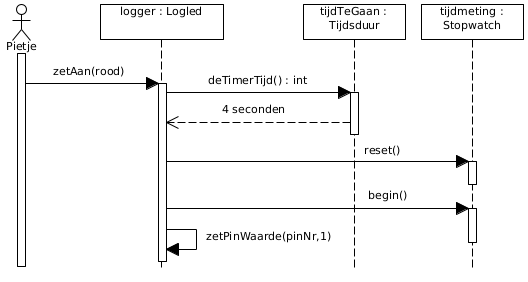
\includegraphics[width=0.8 \linewidth]{figuren/seqZetAan}      %ledPlatform}
  \centering
  \caption{De werking van de methode zetAan.}
  \label{fig:ll_zetAan}
\end{figure} 
 deze nog 4 seconde te gaan heeft. 
 \newpage
 \item De methode \textit{ void zetUit()}. 
 \begin{itemize}
 	\item Stop de stopwatch.
 	\item Haal de stopwachttijd op.
 	\item Breng deze tijd in mindering bij tijdTeGaan.
 	\item Zet de led uit.
 \end{itemize} 
 In het sequentiediagram van figuur \ref{fig:ll_zetUit} wordt een scenario weergegeven wanneer de logled wordt uitgezet
  \begin{figure}[h!]
	\captionsetup{justification=centering}
	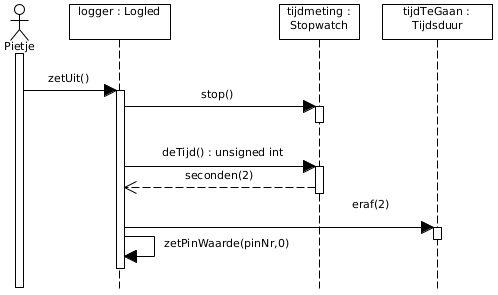
\includegraphics[width=0.8 \linewidth]{figuren/seqZetUit}      %ledPlatform}
\centering
\caption{De werking van de methode zetUit.}
\label{fig:ll_zetUit}
\end{figure} 
nadat deze 2 seconde heeft aangestaan.
\end{itemize}
\newpage
\paragraph{Opdracht}

\begin{enumerate}[label=\alph*]
	\item Implementeer de klasse Logled, zodat de code van listing \ref{lst:loglImpl} zonder compiler errors en warnings werkt.
	\begin{lstlisting}[caption=Een test van de klasse \texttt{LogLed}. ,frame=trbl,firstnumber=1,numbers=left,label={lst:lst:loglImpl}]{Name}
#include <iostream> // nodig voor cout (schrijven naar scherm)
#include <unistd.h>
#include "Logled.h"

using namespace std;

#define RODELEDPIN 135
#define GROENELEDPIN 132

#define TWEE_SEC 2000000
#define DRIE_SEC 3000000

int main() {
	//Een object van de klasse Logled met een maximale 'aan' tijd van 2 seconde 
	Logled logger(RODELEDPIN,"rood","Pietje Puk",0,2);
	logger.zetAan("rood");
	usleep(DRIE_SEC); //wacht 3 seconden
	ll1.zetUit();
	logger.zetAan("rood");//led gaat niet meer aan.
	return 0;
}	
\end{lstlisting}
\item  Pas de main() aan zodat deze eruit ziet als listing \ref{lst:logled2}
\begin{lstlisting}[caption=Twee objecten van de klasse \texttt{LogLed}. ,frame=trbl,firstnumber=1,numbers=left,label={lst:logled2}]{Name}
int main() {
	
	Logled logger(RODELEDPIN,"rood","Pietje Puk",0,4);
	Logled sportled(GROENELEDPIN,"groen","Bb",0,2);
	
	logger.zetAan("rood");
	sportled.zetAan("groen");
	usleep(DRIE_SEC); //wacht 3 seconden
	logger.zetUit();
	sportled.zetUit();
	usleep(TWEE_SEC);//wacht 2 seconden
	logger.zetAan("rood");
	sportled.zetAan("groen");
	usleep(TWEE_SEC);//wacht 2 seconden
	logger.zetUit();
	sportled.zetUit();
	
	return 0;
}	
\end{lstlisting}
Compileer het programma en laat het runnen. Plaats de code (\texttt{.h} en \texttt{.cpp}) file van de klasse \textbf{Logled} in je portfolio.
\newpage
\item Open de vnc viewer, run de DDD debugger (\texttt{ddd ./testlogled}), zet een breakpoint bij het statement  \texttt{usleep(TWEE\_SEC);} (regel 11 van listing \ref{lst:logled2})
\begin{figure}[h!]
\captionsetup{justification=centering}
	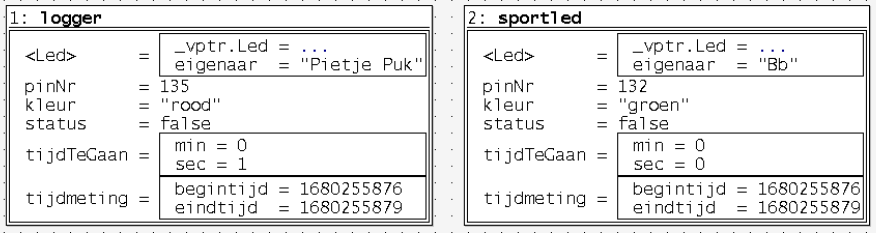
\includegraphics[width=0.85 \linewidth]{figuren/dddTweeLogleds}      
\centering
\caption{Twee objecten van de klasse Logled}
\label{fig:dddTweeLogl}
\end{figure}
en display beide objecten (\texttt{logger} en \texttt{sportled}) van de klasse \textbf{Logled}. Als het goed is krijg je iets te zien zoals figuur \ref{fig:dddTweeLogl}, uiteraard met je \textcolor{red}{eigen} naam.\\
Maak van de afbeelding een screenshot en plaats deze in je portfolio.
\item Voer het programma nog een keer uit en maak gedurende de uitvoer twee \textcolor{BlueViolet}{\textbf{screenshots}} die lijken op figuur \ref{fig:logledOjecten}. Indien Args niet zichtbaar is, kan deze zichtbaar gemaakt worden via Data $\rightarrow$	 Display Arguments (ALT + U).
Led op: De begintijd van \ref{fig:logObjectA} en \ref{fig:logObjectB} zijn hetzelfde, de stopwatch is immers een compositie van logled.
\begin{figure}[h!]
	\centering
	\begin{center} 	
		\begin{subfigure}[b]{0.49\textwidth}
			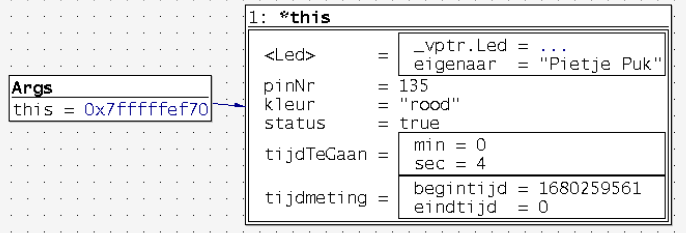
\includegraphics[width=0.95\textwidth]{figuren/ddd_logled_p2a}
			\caption{Logled met composities Tijdsduur en Stopwatch.}
			\label{fig:logObjectA}
		\end{subfigure}
		\begin{subfigure}[b]{0.49\textwidth}
			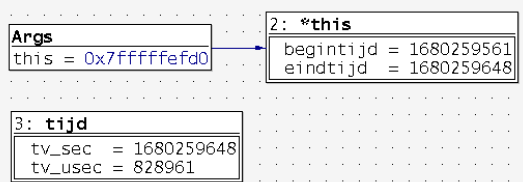
\includegraphics[width=0.95\textwidth]{figuren/ddd_logled_p2b}
			\caption{Van het object stopwatch, de attributen en lokale variabele tijd.}
			\label{fig:logObjectB}
		\end{subfigure}
		\caption{Inhoud van het object logled bij het aanroepen van de  zetUit() en vervolgens stap voor stap naar methode stop() van stopwatch.}
		\label{fig:logledOjecten}   
	\end{center}
\end{figure}
Bij figuur \ref{fig:logObjectB} zie je de waarde van de attributen van het object van de klasse \textit{Stopwatch} waarbij \textit{\textbf{tijd}} een lokale variabele is binnen de methoden \textit{void begin()} en \textit{void stop()} van de klasse Stopwatch.
\end{enumerate}




	\newcommand{\startappendix}{%
%	\cleardoublepage
	\appendix
%	\phantomsection\addcontentsline{toc}{part}{APPENDIX}
%	\part*{APPENDIX}
%	\let\@makechapterhead\@makeschapterhead
}

%\appendix
%\newpage
%\renewcommand{\thechapter}{A}
%\addcontentsline{toc}{section}{Appendices}
%\renewcommand{\thesection}{\Alph{section}}
%\renewcommand{\thesubsection}{\Alph{subsection}}
%\renewcommand{\thesubsection}{\arabic{subsection}
%\renewcommand{\thesection}{\Alph{section}.\arabic{section}}
%\renewcommand{\thesection}{\arabic{section}.\arabic{section}}
%\setcounter{section}{0}

\begin{appendices}
%\section*{Appendices}
%\startappendix

%\printnomenclature
\chapter{Installeren van de practicum omgeving} \label{app:instal}


\section{De VNC viewer}
\label{sec:vnc}
Installeer \href{https://www.realvnc.com/en/connect/download/viewer/}{VNC Viewer} op je laptop. Op de RockPi is VNC Server al geïnstalleerd.
% (op de image van de school is dit al gebeurd).
\begin{comment}
\begin{enumerate}
	\item sudo raspi-config
	\begin{itemize}
		\item Kies 3 Interface Options.
			\begin{itemize}
		\item P3 VNC
		 \item Yes
		 \end{itemize}
	 \item 	Kies 2 Display Option.		
	 	\begin{itemize}
	 	  \item D5 VNC Resolutie of D1 Resolution
	 	  \item DM Mode 85 1280x720 of 1280x1024
	     \end{itemize}
	\end{itemize}
\item Start de VNC viewer op, op je laptop. Vul in het scherm \textit{VNC CONNECT}, zie figuur \ref{fig:winvnc}, het IP adres van de Raspberry PI in.
	\begin{figure}[h!]
	\captionsetup{justification=centering}
	
\includegraphics[width=0.7 \linewidth]{figuren/vncopstart}
	\centering
	\caption{Connect met de PI  maken.}
	\label{fig:winvnc}
\end{figure}
Als het goed is krijg je de grafische omgeving van de PI te zien.
\end{enumerate}
\end{comment}
Start op je laptop de VNC viewer op. Vul in het scherm \textit{VNC CONNECT}, zie Figuur \ref{fig:winvnc}, het IP adres van de RockPi in.
\begin{figure}[h!]
	\captionsetup{justification=centering}
	
\includegraphics[width=1 \linewidth]{figuren/vncopstart}
	\centering
	\caption{VNC verbinding met de RockPi  maken.}
	\label{fig:winvnc}
\end{figure}
\newline
Als het goed is zie je nu de grafische omgeving van de RockPi. Als dit niet werkt, druk dan eens op de \textbf{'Restart\_X'} knop op het uitbreidingsbordje. Dit herstart de X-Windows grafische schil op de RockPi. Probeer daarna opnieuw te verbinden.

	

\section{Het gebruik van 'Visual Studio Code'} \label{app:vsc}
\label{sec:vsc}
\href{https://code.visualstudio.com/docs}{Visual Studio Code} is een cross platform editor uit de Microsoft omgeving. Je kan vanuit je laptop/desktop omgeving direct files editen op een embedded platform zoals een RockPi.Dit principe is te zien in Figuur \ref{fig:winVCS}.
	\begin{figure}[h!]
	\captionsetup{justification=centering}
	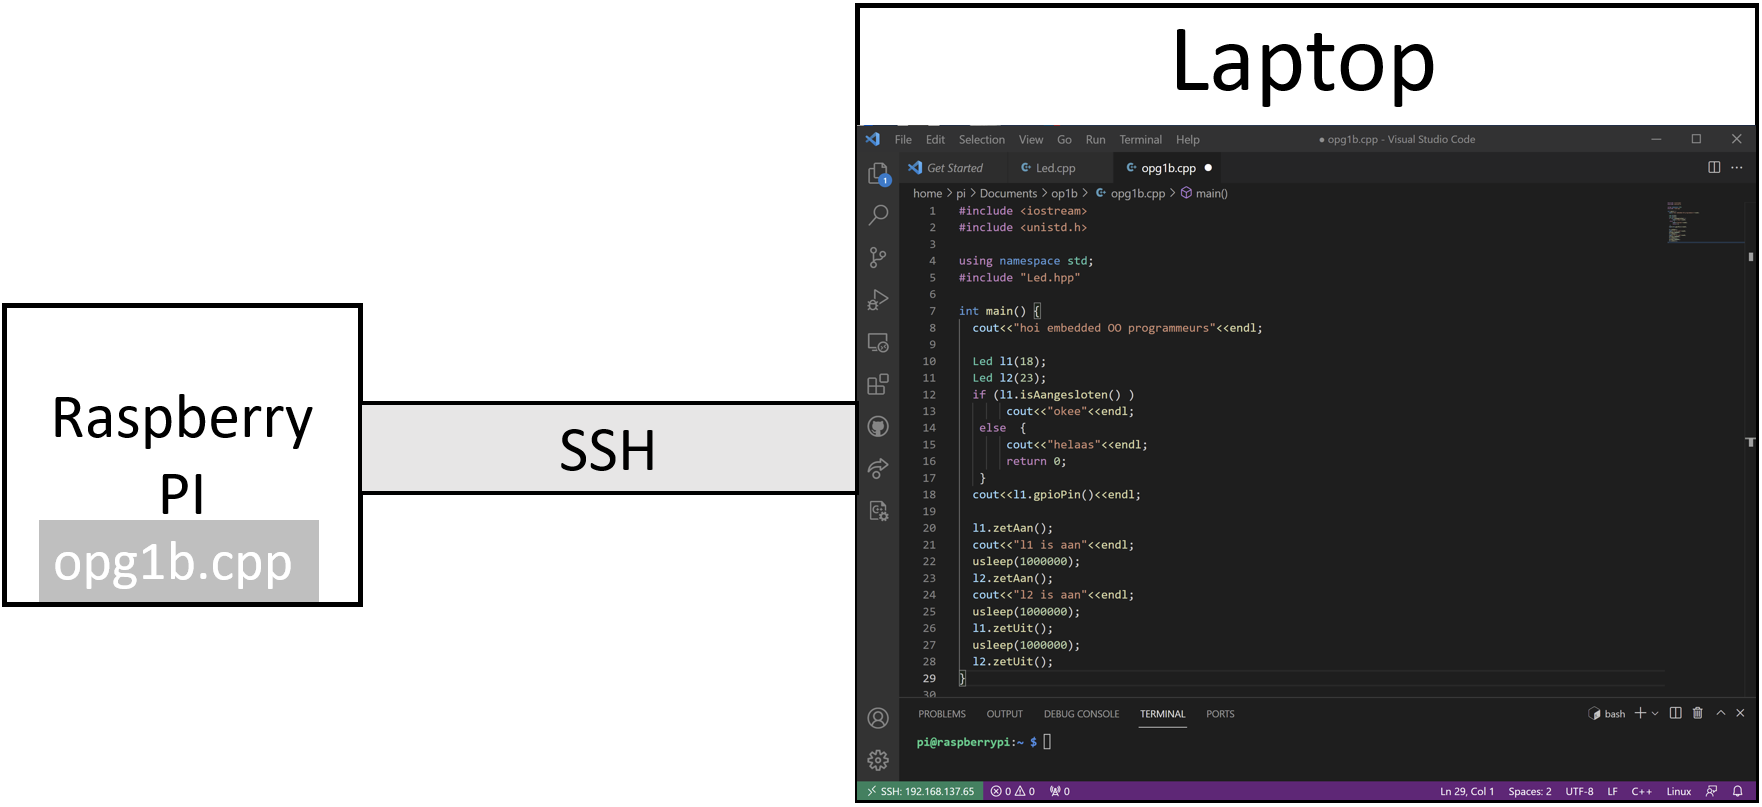
\includegraphics[width=0.65 \linewidth]{figuren/laptopVCS}
	\centering
	\caption{'Visual Studio Code' en de RockPi.}
	\label{fig:winVCS}
\end{figure}
Op de laptop draait 'Visual Studio Code' (VSC) en de source file is de file \texttt{opg1.cpp} op de RockPi. Het compileren kan via VSC, maar kan ook via de terminal in VSC of via een externe terminal b.v Windows PowerShell, KiTTY / PuTTY of een andere.
 

\begin{enumerate}
	\item Download en installeer VCS \href{https://code.visualstudio.com/docs}{Visual studio code}
	\item Bij Visual Studio Code kunnen meerdere extensions geïnstalleerd worden. Het installeren van de \textit{remote SSH} extension kan als volgt gedaan worden:
	\begin{figure}[h!]
	\captionsetup{justification=centering}
	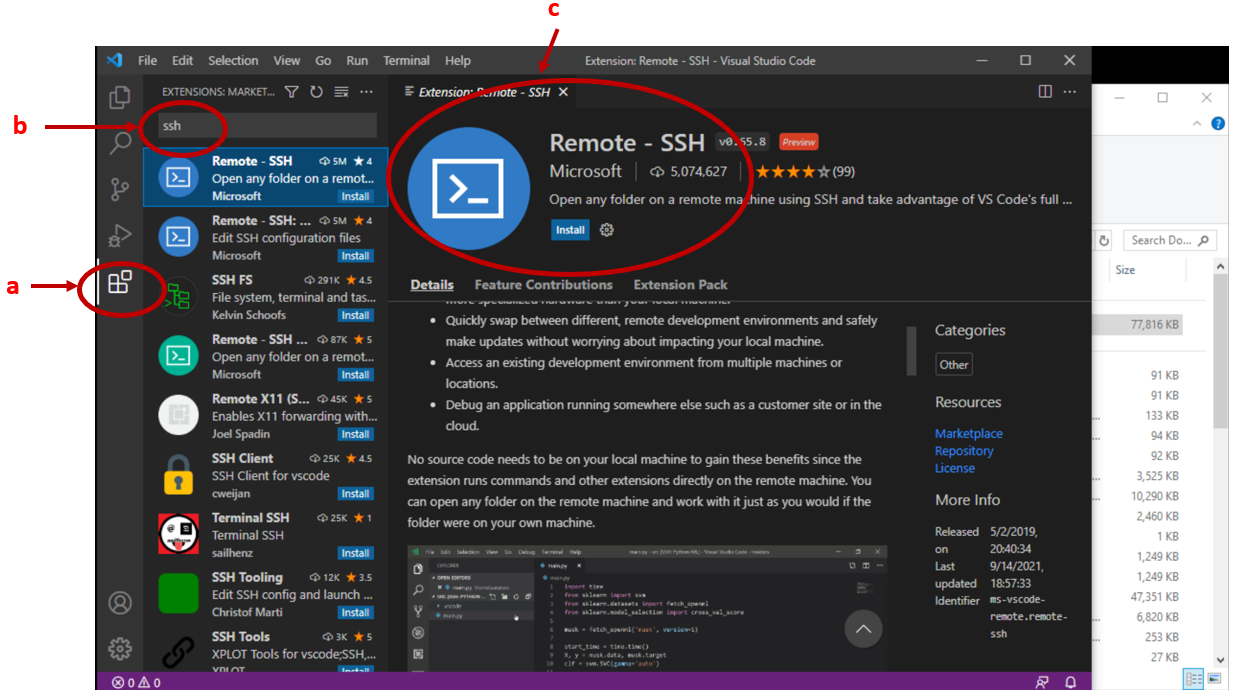
\includegraphics[width=0.6 \linewidth]{figuren/vcsExtSSH}
	\centering
	\caption{Installeren van Remote SSH in VCS.}
	\label{fig:vscEx}
\end{figure}


	\begin{enumerate}
		\item Klik op Extension \img{figuren/extensionIcon} of CTRL + Shift + X
		\item Zoek naar ssh
		\item klik op install
	\end{enumerate}
    \item Verbinding maken met de RockPi.
	\begin{enumerate}
	    \item Ga naar het 'Command Palette' (CTRL+Shift+P). Voer het command Remote-\textcolor{blue}{SSH}:Connect to Host...
	    \begin{figure}[h!]
		\captionsetup{justification=centering}
		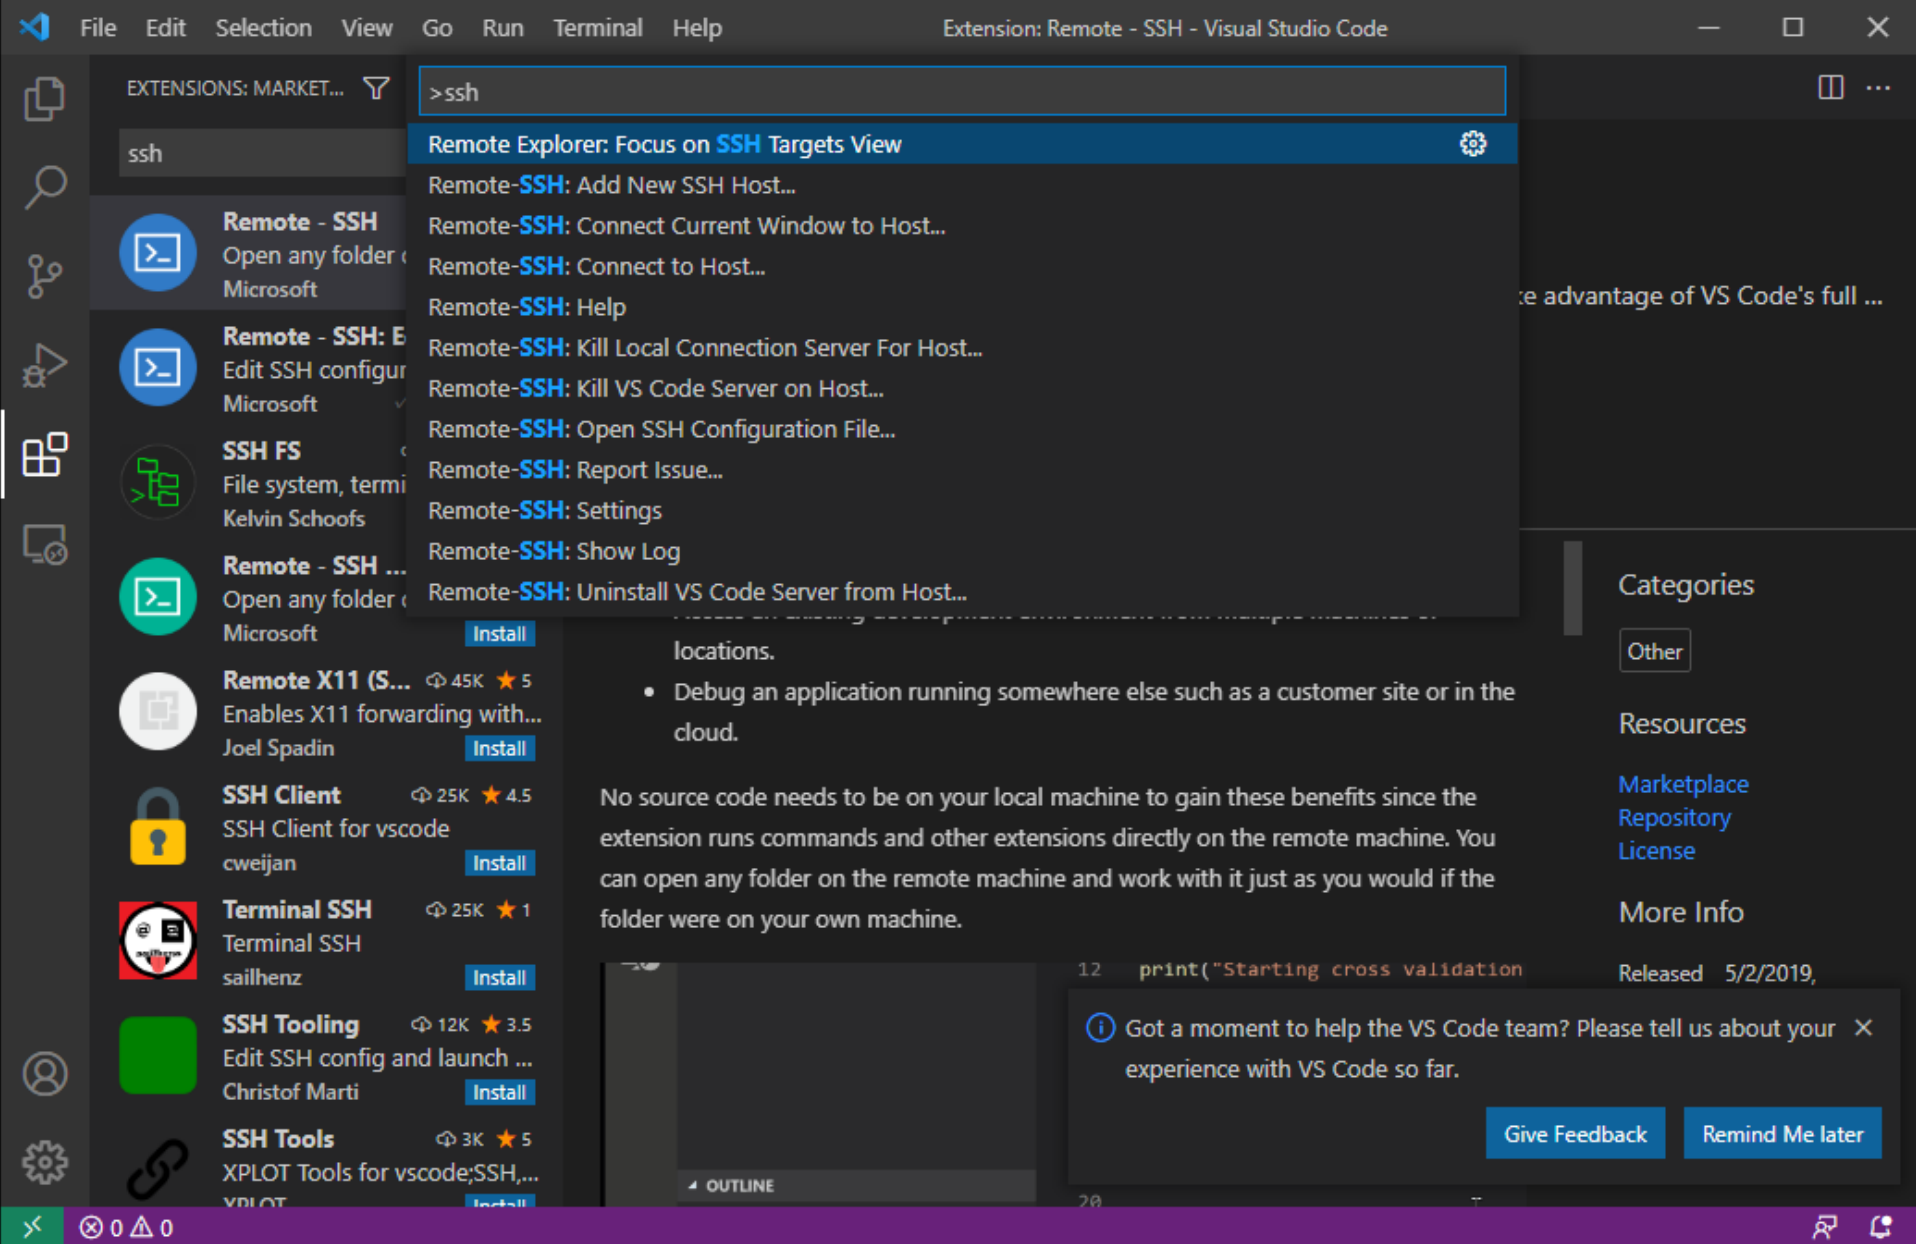
\includegraphics[width=0.6 \linewidth]{figuren/VNCremoteSSH}
		\centering
		\caption{SSH verbinding naar de Host.}
		\label{fig:vscConnect}
	\end{figure}

	Zoals te zien is in Figuur \ref{fig:vscConnect}. VSC komt nu met het scherm zoals te zien is in Figuur \ref{fig:vscAddcon}.
		    \begin{figure}[h!]
		\captionsetup{justification=centering}
		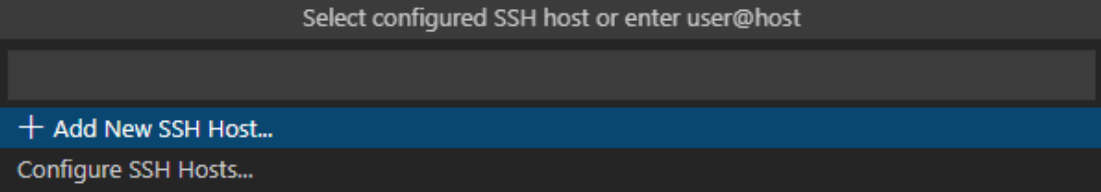
\includegraphics[width=0.6 \linewidth]{figuren/VNCInvoerHost}
		\centering
		\caption{toevoegen van een host.}
		\label{fig:vscAddcon}
	\end{figure}

\item klik op \textit{+ Add New SSH Host}. VSC vraag vervolgens om een ssh command: type in: ssh rock@\textit{\small{ip.nr. van de host}} zoals te zien is in Figuur \ref{fig:vscConIP}. Uiteraard wel met je eigen IP nummer.
		    \begin{figure}[h!]
	\captionsetup{justification=centering}
	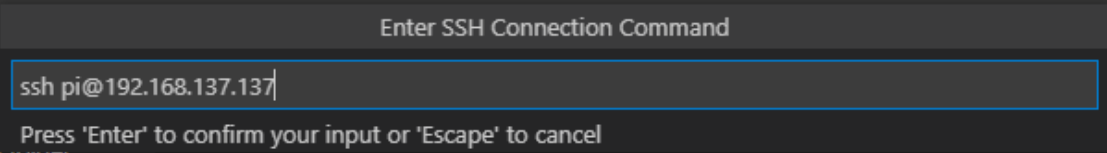
\includegraphics[width=0.7 \linewidth]{figuren/VSCsshCommand}
	\centering
	\caption{connectie maken met de host.}
	\label{fig:vscConIP}
\end{figure}
VSC wil de gegevens opslaan en vraagt vervolgens waar deze opgeslagen moet worden, zoals te zien is in Figuur \ref{fig:vscOpConfig}.
		    \begin{figure}[h!]
	\captionsetup{justification=centering}
	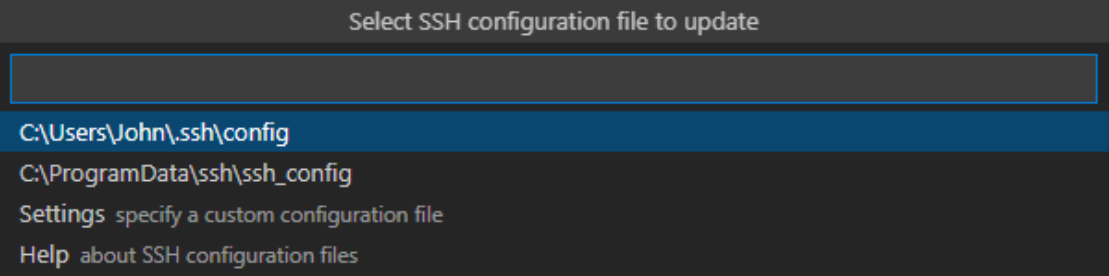
\includegraphics[width=0.7 \linewidth]{figuren/VSCconfigFile}
	\centering
	\caption{waar de gegevens moeten worden opgeslagen.}
	\label{fig:vscOpConfig}
\end{figure}

VSC slaat de gegevens op en geeft een bericht (rechtsonder) of de config file geopend moet worden of dat een connectie gemaakt moet worden. Maak een connectie, VSC komt vervolgens met de vraag of je zeker weet dat je doorgaat, zoals Figuur \ref{fig:vscOpContinue} laat zien.
		    \begin{figure}[h!]
	\captionsetup{justification=centering}
	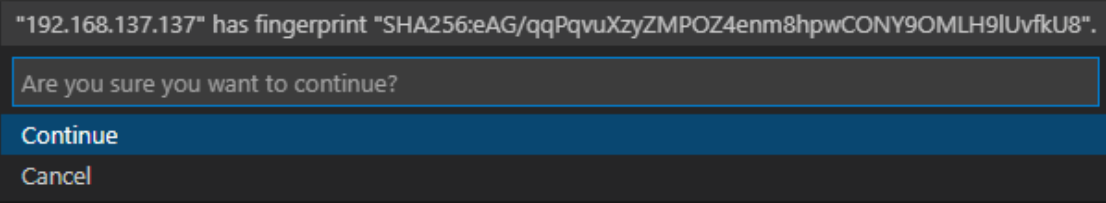
\includegraphics[width=0.7 \linewidth]{figuren/VSCcontinue}
	\centering
	\caption{waar de gegevens moeten worden opgeslagen.}
	\label{fig:vscOpContinue}
\end{figure}

	     \item Klik op \textit{Continue}. VSC vraagt om een password zoals Figuur \ref{fig:vscVrPasswd} laat zien. Het password is: \textit{rock} 
		    \begin{figure}[h!]
	\captionsetup{justification=centering}
	
\includegraphics[width=0.7 \linewidth]{figuren/VSCpasswd}
	\centering
	\caption{invullen van een password.}
	\label{fig:vscVrPasswd}
\end{figure}	

Het kan zijn dat een foutmelding gegeven wordt zoals b.v. in Figuur \ref{fig:vscfout1} laat zien. 
		    \begin{figure}[h!]
	\captionsetup{justification=centering}
	
\includegraphics[width=0.6 \linewidth]{figuren/VSCfout1}
	\centering
	\caption{een foutmelding.}
	\label{fig:vscfout1}
\end{figure}	
Raak niet in paniek en probeer desgewenst weer opnieuw.
\item Maak een nieuwe terminal aan (Terminal $\rightarrow$ New Terminal). 
\begin{figure}[h!]
	\captionsetup{justification=centering}
	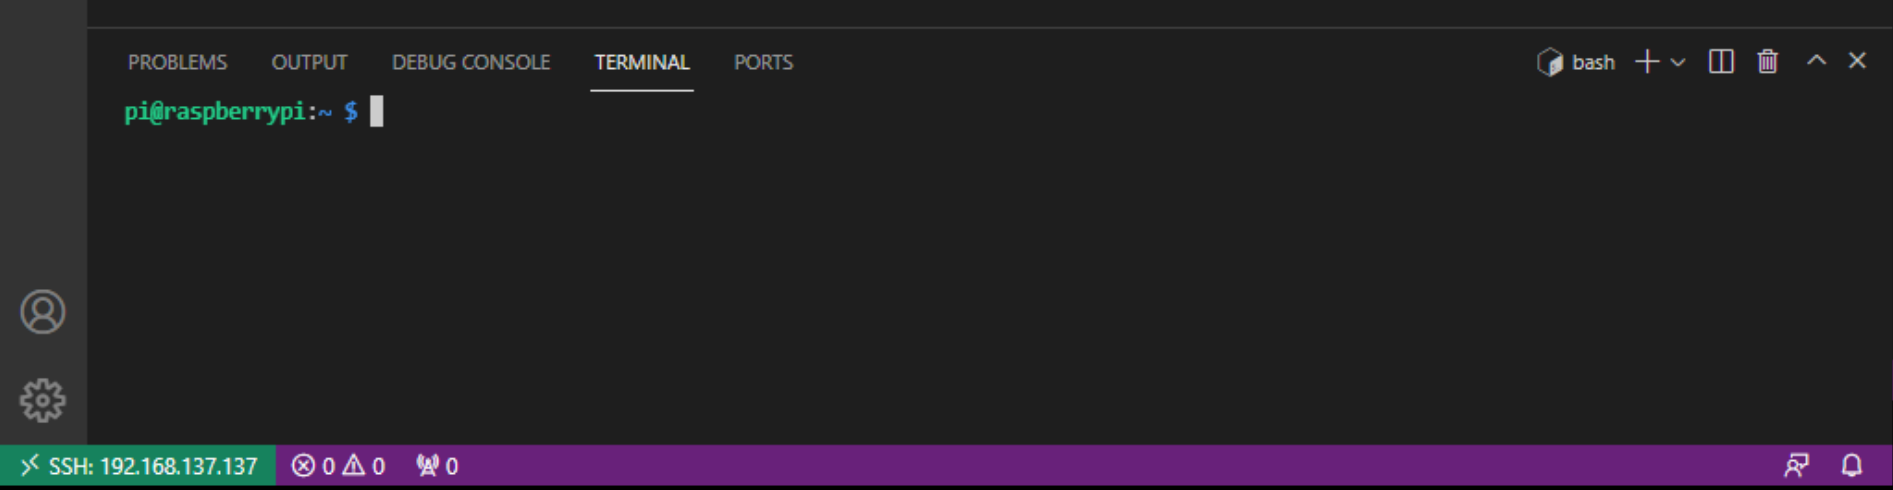
\includegraphics[width=0.6 \linewidth]{figuren/VSCnewTerminal}
	\centering
	\caption{Een geopende terminal in VSC.}
	\label{fig:vscnewTerm}
\end{figure}	
Als het goed is verschijnt de terminal in het onderste deel van VSC met een ssh verbinding naar de RockPi, zoals Figuur \ref{fig:vscnewTerm} laat zien. 
\begin{enumerate}
	\item Met het \textit{ls} commando vraag je de listing op van de huidige directory.
	\item Met het \textit{pwd} commando wordt het pad van de huidige directory zichtbaar.\\
	\textit{pwd} \textless enter\textgreater $\rightarrow$  /home/rock.
	\item  Met het \textit{cd} commando wordt naar een directory gegaan\newline
	(LET OP: Ik ga er van uit dat je een \hyperlink{chp:USBstick}{USB stick} gebruikt!):\\  
	\textit{cd Documents} \textless enter \textgreater $\rightarrow$  
	\textcolor{green}{rock@rockpi-4b}:\textcolor{blue}{$\mathtt{\sim}$/Documents \$}
	\item  Met het \textit{mkdir} commando wordt een directory aangemaakt.\\
	Maak in de directory \textit{Documents} een directory \textit{intro} aan.\newline \\
	Ga naar de directory \textit{intro} (\textit{cd intro}) en vraagt het path op.\\
	\textit{pwd}  $\rightarrow$  /home/rock/Documents/intro
	
\end{enumerate}

\end{enumerate}  
	     \item Het eerste programma op de RockPi.
	     \begin{enumerate}
	     	\item VSC werkt voornamelijk met directory's (folders). Het openen van een folder in VSC op de RockPi kan door te klikken op Explorer \img{figuren/VSCiconeExpl} of Ctrl+Shift+E. VSC opent een scherm, zoiets als \textcolor{red}{\textbf{[1]}} in Figuur \ref{fig:vscOpenFolder}.
		    \begin{figure}[h!]
	\captionsetup{justification=centering}
	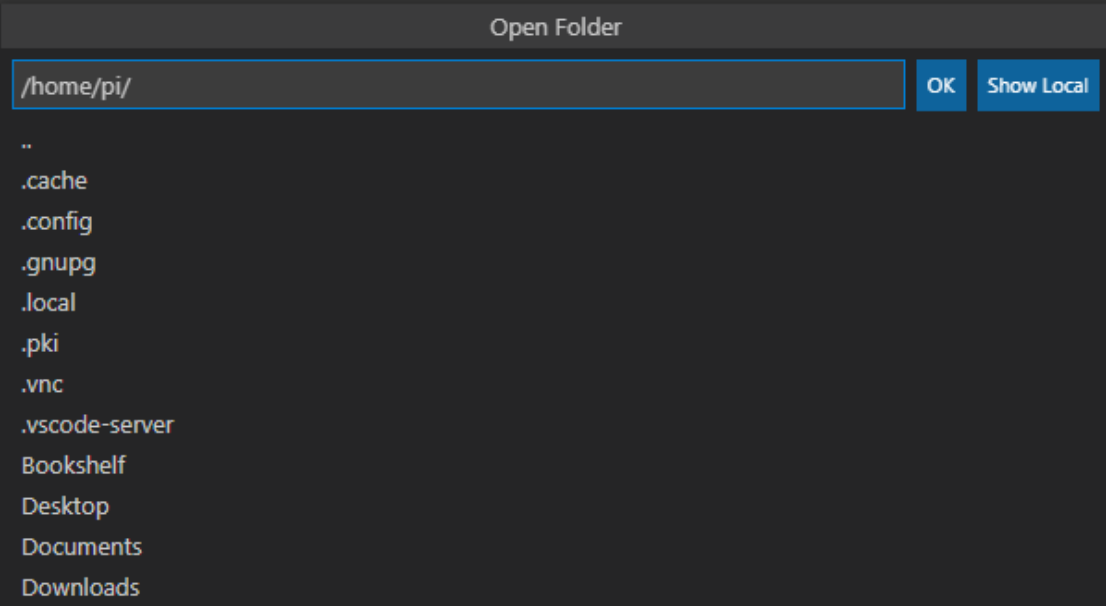
\includegraphics[width=0.8 \linewidth]{figuren/VSCopenFolder}
	\centering
	\caption{De directory die geopend moet worden.}
	\label{fig:vscOpenFolder}
\end{figure}
\newline 
Voer bij \textcolor{red}{\textbf{[2]}} de directory \textit{/home/rock/Documents/intro} in en klik op 'OK'.
VSC kan vragen of je de auteur vertrouwt. Klik op 'Yes'. \\
 In het \textit{EXPLORER} veld verschijnt vervolgens de nu nog lege werkdirectory, zoals in Figuur \ref{fig:vscExploVeld} te zien is.
 	\begin{figure}[h!]
        	\captionsetup{justification=centering}
 	        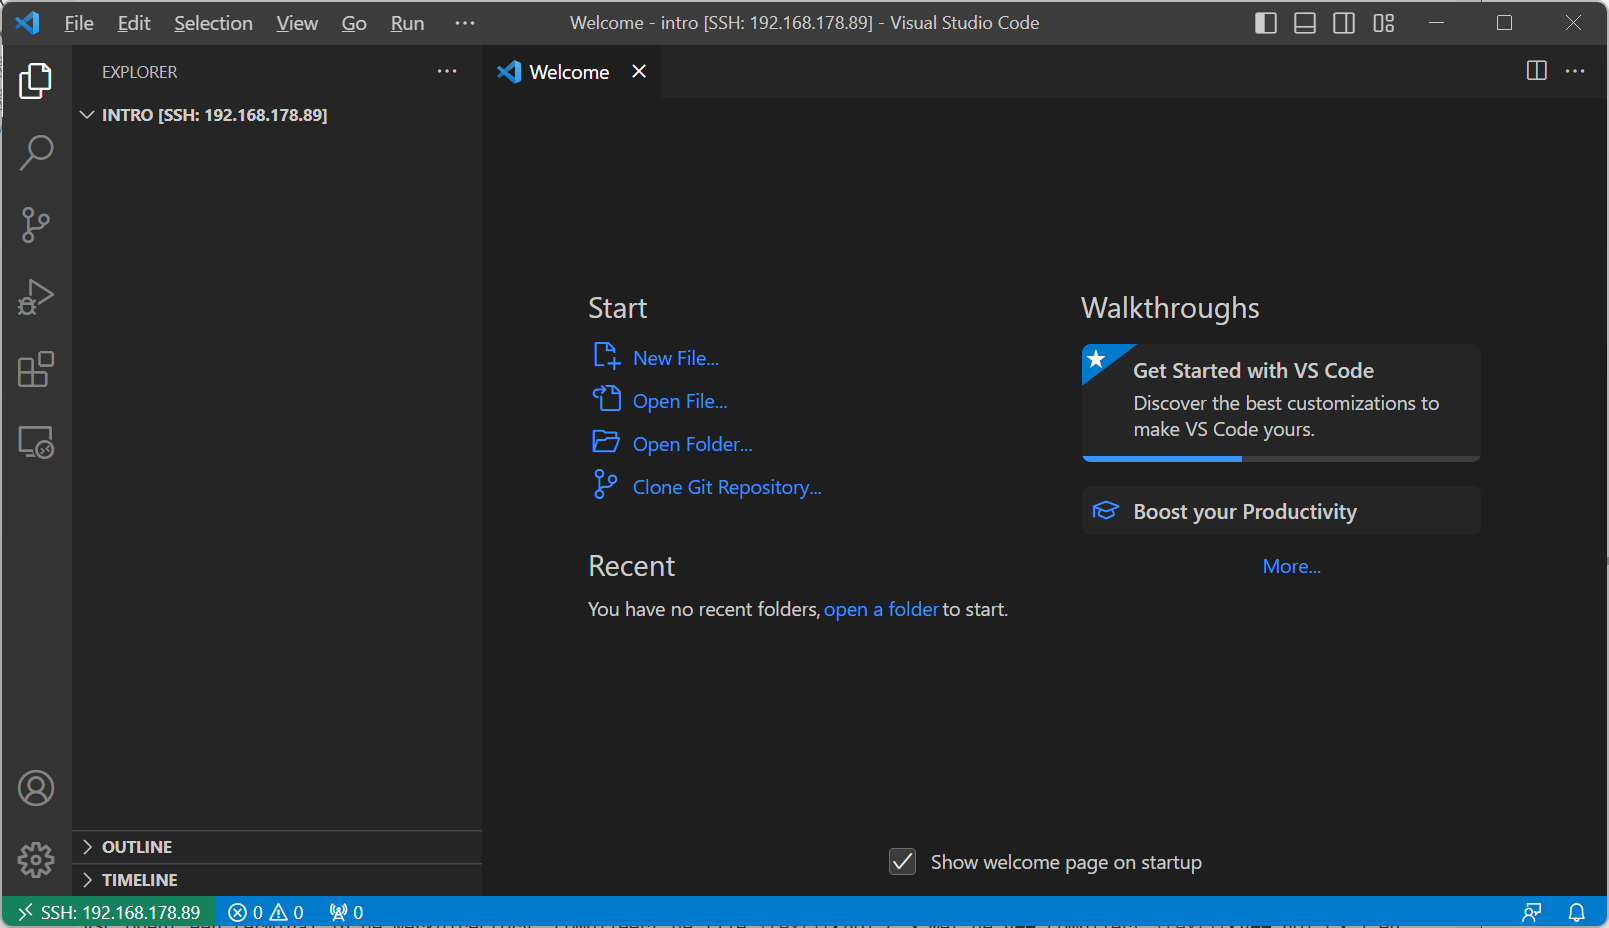
\includegraphics[width=0.6\linewidth]{figuren/VSCexplorerveld}
 	        \centering
 	        \caption{In het EXPLORER veld is de werkdirectory te zien.}
 	         \label{fig:vscExploVeld}
     \end{figure} 
\newpage % Gert
\item Het programma van listing \ref{lst:hoi} kan:  gecreëerd worden door een nieuwe file \textit{hoi.cpp} aan te maken [i], gedownload worden van Brightspace [ii] of gecloned worden van Github [iii].
\begin{enumerate} %{itemize}
 \item
 Klik op New File  \img{figuren/VSCmakeFile} en geef de filenaam \textit{hoi.cpp}.
	 Type/kopieer de tekst van Listing \ref{lst:hoi} in de file \textit{hoi.cpp}
	 
	 \begin{lstlisting}[caption= het meest gebruikte voorbeeld programma.,captionpos=b ,label={lst:hoi}]
#include <stdio.h>
int main(){
	
	printf("Hoi programmeurs van de wereld\n");
	return 0;
}
\end{lstlisting}   	
\item
Download de file \textit{hoi.cpp} van Brightspace en plaats deze in de directory. Het laatste kan zelfs gedaan worden door middel van slepen van de file.
\item
Via git: \textit{git clone~  - -branch intro https://github.com/Johnny63Vi/oopr1.git}\footnote{bij uitvoering geen spatie tussen - -}
Het nadeel van deze methode is dat een directory oopr1 wordt aangemaakt waarin de file komt te staan.
\end{enumerate} %{itemize}

\item Open de bestaande terminal of open een nieuwe terminal \textit{Ctrl+Shift+`}.\newline 
VSC opent een terminal in de werkdirectory. compileer de file \textit{hoi.cpp} met de g++ compiler (\textit{g++ hoi.cpp}) en run het gecompileerde programma \textit{./a.out}.\\
Uiteraard kan ook gekozen worden voor een externe terminal zoals, \textit{Windows PowerShell}, \textit{PuTTY}, etc.\\
Delete a.out (\texttt{rm a.out}). 
	     \end{enumerate}

      \item Compileren via VSC.\\
     Je kan het programma ook via VSC laten compileren.
     
     \begin{enumerate}
     	\item  Daarvoor moet de de C++ omgeving in Visual Studio Code worden geïnstalleerd (is al gedaan bij de RockPi):
     	\begin{enumerate}
     		\item Klik op Extension \img{figuren/extensionIcon} of Ctrl+Shift+X.
     		\item Type in C++ en installeer de C++  \img{figuren/cPlusIcon}, het Extension pack en C/C++ Themes.
        \end{enumerate}
     	\item Activeer het tabblad \textit{hoi.cpp}.
     	\item Klik op \textit{Terminal $\rightarrow$ Configure Default Build Task...}. VSC komt met een scherm zoals Figuur \ref{fig:vscComp}.
\begin{figure}[h!]
	\captionsetup{justification=centering}
	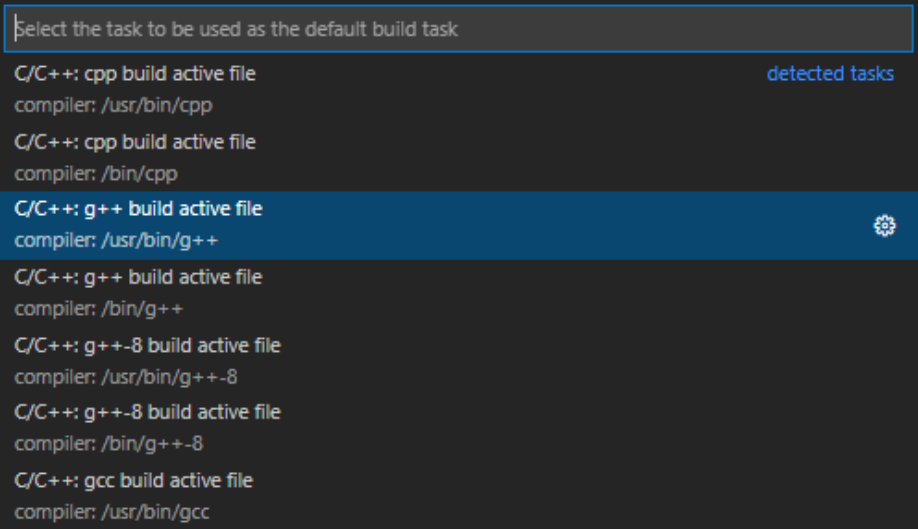
\includegraphics[width=0.6 \linewidth]{figuren/VSCcompile}
	\centering
	\caption{Het kiezen van de compiler.}
	\label{fig:vscComp}
\end{figure}     	
Kies voor \texttt{C/C++: g++ build active file}.
VSC maakt nu een task.json file aan waarin de gegevens betreffende compiler worden opgeslagen.
\item Activeer opnieuw \textit{hoi.cpp} tab. Ga naar Terminal $\rightarrow$ Run Build Task... of \textit{Ctrl+Shift+B}. VSC zal nu \textit{hoi.cpp} compileren.

\item Het gecompileerde programma kan nu gerund worden in b.v. een terminal. Open een terminal of maak een nieuwe terminal aan \textit{Ctrl+Shift+`} en run hoi (\texttt{./hoi}).
\end{enumerate}
     
     \item Run/Debug via VSC.\\
     Je kan een programma ook direct via VSC laten runnen en Debuggen.
     \begin{enumerate}
     	\item Activeer het tabblad \textit{hoi.cpp}.
     	\item Klik op \textit{Run and Debug (Ctrl+Shift+D)} \img{figuren/VSCiconeRunDebug} en vervolgens op\\ \colorbox{NavyBlue}{\textcolor{White}{\textbf{Run and Debug}}}. Afhankelijk van instellingen kan VSC kiezen voor Figuur \ref{fig:kzComp}. 
   Kies hierbij C++ (GDB/LLDB), VSC laat hierna Figuur \ref{fig:kzCompVer} zien. Kies voor: \textit{g++ - Build and Debug active file \small{compiler /usr/bin/g++}}.
   VSC maakt o.a. \textit{launch.json} file aan. Hierin worden diverse gegevens met betrekking tot de compiler/debugger in opgeslagen. \\
   Het zou ook kunnen dat VSC de DEBUG CONSOLE opent. 
      
   \item Klik op tabblad hoi.cpp en plaats vervolgens een breakpoint voor regel 4 (linker muisklik voor regel 4) (printf), een rode stip verschijnt voor de 4. 
   \item Start de debugger:Run $\rightarrow$ Start Debugging of F5 of klik op \img{figuren/VCRrunDebug}. Het programma wordt op de RockPi uitgevoerd en stopt op regel 4, zoals te zien is in Figuur \ref{fig:vscDebugVld}.\newline
\end{enumerate}
     \begin{figure}[h!]
	\centering
	\begin{center} 	
		\begin{subfigure}[b]{0.44\textwidth}
			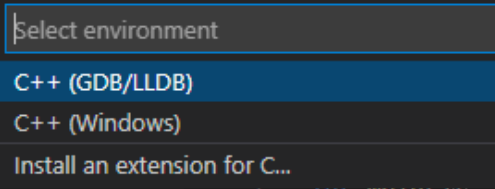
\includegraphics[width=0.85\textwidth]{figuren/VSCksGDB}
			\caption{Keuze welke compiler}
			\label{fig:kzComp}
		\end{subfigure}
		\begin{subfigure}[b]{0.45\textwidth}
			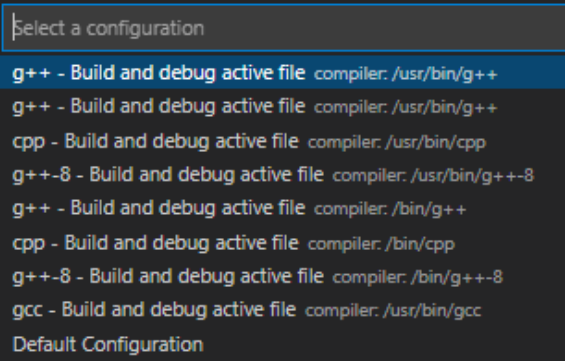
\includegraphics[width=0.95\textwidth]{figuren/VSCKsGcc}
			\caption{Keuze versie compiler}
			\label{fig:kzCompVer}
		\end{subfigure}
		\caption{Keuze compiler te gebruiken door VSC}
		\label{fig:kzcompiler}   
	\end{center}
\end{figure}

\begin{figure}[h!]
\captionsetup{justification=centering}
\includegraphics[width=0.8 \linewidth]{figuren/VSCdebugVeld}
\centering
\caption{Debuggen met VSC.}
\label{fig:vscDebugVld}
\end{figure}     
   Met behulp van de debugknoppen \includegraphics[width=0.3 \linewidth]{figuren/VSCDebugKnoppen} kan stap voor stap door het programma gelopen worden. Hieronder staan de belangrijkste:

\begin{table}[h!] % [ht]
	\begin{tabular*}{6.6in}{ c | c | l }
		\hline
		\includegraphics[width=0.05\textwidth, height=8mm]{figuren/F5-Continue} & 'Continue (F5)' & Vervolg het programma. \\ \hline
		\includegraphics[width=0.05\textwidth, height=8mm]{figuren/F10-StepOver} & 'Step Over (F10)' & \specialcell{Stap over de volgende regel heen\\(ook als het een functieaanroep is).}  \\ \hline
		\includegraphics[width=0.05\textwidth, height=8mm]{figuren/F11-StepInto} & 'Step into (F11)' & \specialcell{Voer de regel uit. Als het een functieaanroep is: ga de functie in.\\ \textit{Als het een systeemfunctie is, dan wordt het vaak onbegrijpelijk!}}  \\ \hline
	\end{tabular*}
\end{table}

   
     \end{enumerate}
     
	

\hypertarget{LinuxTipsTrics}{}
\chapter{Tips\&Tricks\&Troubleshooting voor Linux omgeving} \label{app:linux}
\section{Troubleshooting}
\textbf{\textit{Geen beeld in VNC}}.\newline 
Je hebt VNC opgestart, maar na een tijdje heb je geen beeld meer.
Waarschijnlijk komt dat door de screensaver. VNC reageert niet op op een `virtuele` toetsenbord of muis. Druk dan het knopje \textbf{`restart\_x`} in log opnieuw in op VNC. 
\textit{De screensaver wordt uitgeschakeld als je na het inloggen in VNC een terminal venster opent.} Daarmee worden direct een paar commando's uitgevoerd waarmee de screensaver wordt uitgezet.\newline
\textbf{\textit{DDD `doet raar`}}.\newline 
De instellingen van de DDD debugger staan in de folder .ddd die staat in de home directory (\textit{/home/rock}). Soms is het eenvoudiger om deze directory te deleten dan de instellingen aan te passen (tips: \texttt{ls -al $\sim$} en \texttt{rm -rf $\sim$/.ddd}).

\section{Tips} \label{app:tips}
\textbf{\textit{Je kunt de tips en trucs toepassen bij de commando's in \ref{app:commands}}}

\begin{itemize}
	\item 
	Linux is in tegenstelling tot Windows ‘case-sensitive’. Het maakt dus verschil of je hoofdletters of kleine letters gebruikt. Voorbeeld: Als je map \texttt{Documents} heet, dan werkt \texttt{cd Documents} wel en \texttt{cd documents} niet.
	\item 
	Tip bij het invoeren van map- en bestandsnamen: tik de eerste 3 letters in en druk de Tab toets in, Linux vult dan automatisch de rest van de naam in. Voordeel: je hoeft minder te tikken en het is gelijk een foutcontrole.
	\item 
	Op en neer pijltjestoetsen in de terminal: door vorige commando's heen gaan.
	\item
	Nog een verschil met Windows; Windows werkt met bestandsextensies: *.exe is een uitvoerbaar (executable) betand. In Linux doet de extensie er niet toe, maar zet je met \texttt{chmod +x} het 'executable' bitje aan, een attribuut op het bestand.
	\item  
	Hulp vragen bij commando’s: \texttt{<\textit{commando}> --help}. Voorbeeld: \texttt{ls  --help}
	Uitgebreidere informatie: \texttt{man <\textit{commando}>}. Voorbeeld: \texttt{man ls}\newline
	Voor de bedieningstoetsen van \texttt{man} druk ‘h’.
	\item 
	\href{https://phoenixnap.com/kb/linux-sudo-command}{Uitleg en gebruik van het sudo commando}  ('\textbf{Su}per \textbf{U}ser \textbf{Do}'); admin rechten.
	\item
	Zoeken in het bestandssysteem: \texttt{sudo find / -name \textit{<bestandsnaam>}}
	zoekt naar \texttt{\textit{<bestandsnaam>}} vanaf de root '/' in het gehele bestandssysteem.
	\item 
	\href{https://linuxconfig.org/filesystem-basics}{Uitleg van- en navigeren door het bestandssysteem.}
	\item
	Wil je meer uitleg, \href{https://duckduckgo.com/?q=linux+command+cheatsheet}{zoek dan naar 'Linux Command Cheatsheet'}. \newline
	Ik vind \href{https://linuxconfig.org/linux-commands-cheat-sheet}{deze uitleg} wel prettig.
\end{itemize}

% \break
\section{Linux commando's (zie ook tips in \ref{app:tips})}\label{app:commands}

%\begin{table}[ht] %[h!]
	\begin{tabular}{|l|l|}
		\hline
		%\multicolumn{2}{|l|}{Linux commando's}    \\ \hline
		Commando & Uitleg \\ \hline
		\texttt{ls \textbf{-l}} & \textbf{L}ange directory listing - Opvragen van bestanden in een directory  \\ \hline
		\texttt{cd} & change directory; \texttt{cd ..} betekent 1 niveau omhoog naar de root '/' \\ \hline
	    \texttt{cp} & copy \\ \hline
	    \texttt{rm} & remove - Verwijderen van bestanden en mappen. \\ \hline
	    \texttt{mv} & move - Verplaatsen van bestanden en mappen. \\ \hline
	    \texttt{cat} & bestand bekijken \\ \hline
	    \texttt{pwd} & In welke directoy sta ik? ('present working directory') \\ \hline
	    \texttt{mkdir} & make directory \\ \hline
		\texttt{rmdir} & remove (lege) directory \\ \hline
	    \texttt{history} & Laat lijst zien van laatst uitgevoerde commando's \\ \hline
	    \texttt{sudo} & Zet dit vóór je commando om het met admin rechten uit te voeren.\\
	    ~ & \emph{Alle onderstaande commando's hebben \textbf{sudo} nodig!} \\ \hline
	    \texttt{chmod} & (lees/schrijfrechten wijzigen, +x maakt bestand executable. \\ \hline
	    \texttt{chown} & eigenaar van bestand / map wijzigen \\ \hline
	    \texttt{journalctl} & journalctl -n 30 laat de laatste 30 regels linux systemlog zien. \\ \hline
	    \texttt{reboot} & opnieuw opstarten \\ \hline
	\end{tabular}
%\end{table}
% Lelijke manier om tabel bovenaan de pagina te zetten (Gert). Standaard uitlijning is onderaan pagina.
~\\~\\~\\~\\~\\~\\~\\~\\~\\~\\~\\~\\~\\~\\~\\~\\~\\~\\~\\~\\~\\~\\~\\~\\

\break
\section{Uitleg GPIO poorten in Linux}\label{app:gpiolinux}
In Linux wordt alles gerepresenteerd als een bestand. Of het nu een volledige disk of een device is, je kunt het als een bestand openen en lezen en schrijven. Dit geldt ook voor GPIO pinnen (‘General Purpose Input/Output’ pinnen). Deze pinnen gebruik je op dezelfde manier als de pinnen van een microcontroller (denk aan een Arduino Uno, of een Microbit). Je kunt pinnen als uitgang zetten en hoog of laag maken, of als ingang instellen en uitlezen of een pin hoog of laag is (en nog meer, bijvoorbeeld pull-up en pull-down en reageren op events, maar dat gaan we niet behandelen).\newline
Omdat pinnen gerepresenteerd worden door bestanden, geldt ook dat er rechten op gezet worden in het bestandssysteem. Meestal kan een standaard gebruiker (zoal ‘rock’) er niet bij. Alleen ‘root’ kan er standaard bij. Voor het practicum hebben we de rechten zo ingesteld dat gebruiker ‘rock’ standaard gebruik kan maken van de op de breakout board beschikbare pinnen.\newline
Voorbeeld van de handelingen om een pin in te stellen en uit te lezen of aan te sturen, het hekje ‘\#’ aan het begin van de regel geeft aan dat het commentaar (uitleg) is:

\begin{lstlisting}[language=bash]
# GPIO pin 135 (de rode led) aanzetten:
echo 135 > /sys/class/gpio/export
# GPIO pin 135 (de rode led) als uitgang instellen:
echo out > /sys/class/gpio/gpio135/direction
# GPIO pin 135 (de rode led) hoog maken:
echo 1 > /sys/class/gpio/gpio135/value
# 1 seconde wachten
sleep 1
# GPIO pin 135 (de rode led) laag maken:
echo 0 > /sys/class/gpio/gpio135/value
\end{lstlisting}
	
Je kunt ook de hele bestandstructuur van de pin bekijken:
\begin{lstlisting}[language=bash]
rock@rockpi-4b:~$ ls -l /sys/class/gpio/gpio135/
total 0
-rwSrwSr-- 1 root gpio 4096 Mar 12 18:49 active_low
lrwxrwxrwx 1 root gpio    0 Mar 12 18:49 device -> ../../../pinctrl
-rwSrwSr-- 1 root gpio 4096 Mar 12 18:49 direction
-rwSrwSr-- 1 root gpio 4096 Mar 12 18:49 edge
drwsrwsr-x 2 root gpio    0 Mar 12 18:49 power
lrwxrwxrwx 1 root gpio    0 Mar 12 18:49 subsystem -> ../../../../../class/gpio
-rwSrwSr-- 1 root gpio 4096 Mar 12 18:49 uevent
-rwSrwSr-- 1 root gpio 4096 Mar 13 10:55 value
\end{lstlisting}
	
En een bepaalde status uitlezen (in dit geval of de pin als ingang of uitgang is ingesteld):
\begin{lstlisting}[language=bash]
rock@rockpi-4b:~$ cat /sys/class/gpio/gpio135/direction
out
rock@rockpi-4b:~$
\end{lstlisting}
	
Tot zover de uitleg. Ik laat GPIO pin als ingang en gebruik met PWM voor nu achterwege. Als je daar meer van wilt weten, kijk dan even naar het zelftest scriptje: \texttt{sudo cat /usr/local/bin/pwmtest.sh} 


%\input{deRockOmgeving}
%\input{problemen}
%\input{codeVoorDeChallenge}
%\input{microSQL}


%\input{mc}
%\input{answ_questionnare}

% \input{troubleshooting}

\end{appendices}

	\begin{comment}
	\maketitle
	
	
	\tableofcontents
	
	\let\cleardoublepage\clearpage
	\let\cleardoublepage\clearpage
	
	
%	\chapter{Inleiding}\label{chap:inl}
Voor het practicum OOPR1 zijn (ongeveer) 25 RockPi’s beschikbaar. Dit zijn Raspberry Pi achtige ‘Single Board Computers’ die met een Linux variant werken, in dit geval Debian 10. De RockPi’s zijn aangeschaft omdat Raspberry Pi’s niet leverbaar (of te duur) waren.
Tijdens het practicum gebruik je een RockPi van school. Je kunt deze alleen op school gebruiken, je mag hem niet meenemen naar huis. Dat is dan ook het belangrijkste nadeel.

Het gebruik van de RockPi heeft een aantal voordelen:
\begin{itemize}
\item Je hoeft zelf niets aan te schaffen
\item Je werkt onder gecontroleerde omstandigheden: de verstrekte RockPi bevat alles wat nodig is voor het practicum. Dat betekent dat jij- of de docent niet eerst moet puzzelen om de omgeving aan de praat te krijgen.
\end{itemize}

\hypertarget{USBinleiding}{}
Bij het practicum heb je \textit{je eigen} USB stick nodig om je bestanden op te zetten (\textit{geen gedeelde!}). Een USB stick van 1GB is goed genoeg (128+ MB). Groter mag, maar is zinloos.
\begin{itemize}
\item Je werkt op je eigen \hyperlink{chp:USBstick}{USB stick} en niet op het bestandssysteem van de RockPi. 
\item Na afloop van het practicum lever je de RockPi in zonder daar bestanden op achter te laten. 
\item Ga er vanuit dat de RockPi’s na een practicum gewist worden!
\end{itemize}
\colorbox{yellow}{\textcolor{red}{\textbf{\textit{Dit is géén security practicum, de RockPi's zijn slecht beveiligd.}}}}\\
\colorbox{yellow}{\textcolor{red}{\textbf{\textit{Ga dus niet klooien en klieren op de RockPi van iemand anders.}}}}\\
\colorbox{yellow}{\textcolor{red}{\textbf{\textit{Als je overlast veroorzaakt zal de docent je uit het practicum verwijderen!!}}}}

\section{Voorbereiding - Software installeren}
Zorg dat je vóór het practicum de benodigde software geïnstalleerd hebt.
Zie Bijlage \ref{app:instal} voor software installatie.
\newpage

\begin{comment}
\begin{itemize}
\item Installeer Github Desktop: \url{https://desktop.github.com/}
\item Vanuit Github Desktop, druk Ctrl+Shift+O voor 'Clone repository' en voeg de repository \textbf{JohnVi-hhs/oop} toe.
\item Installeer 'Visual Studio Code' (VSC) volgens de instructies in \newline \url{https://github.com/Grrtzm/OOPR1} \textit{(moet nog aangepast worden)}
\item Download en installeer de VNC viewer:  \newline \url{https://www.realVNC.com/en/connect/download/combined/}
\item (Optioneel maar wel handig) Download en installeer de SSH client KiTTY  \newline \url{https://www.fosshub.com/KiTTY.html} \newline
KiTTY is een opvolger van PuTTY. Het grote voordeel is dat KiTTY automatisch opnieuw verbinding maakt als de verbinding even verbroken is geweest.
\end{itemize}
\end{comment}

\section{Eerste gebruik van de RockPi}
We gaan er van uit dat je de RockPi in lokaal D2.001 of D2.003 van HHS Delft gebruikt. \newline
De RockPi is al ingesteld voor Wi-Fi netwerk in D2.001: \textbf{Lab001}. \newline
Log ook met je laptop in op dit netwerk. Het password is \textbf{Lab001WiFi}. \newline
In Figuur \ref{fig:netw} wordt weergegeven hoe de RockPi op het lab netwerk is aangesloten.
\begin{figure}[h!]
	\centering
	\begin{center} 	
		\includegraphics[width=0.4\textwidth]{figuren/laBnetwork}
		\caption{De RockPi in het lab netwerk}
		\label{fig:netw}   
	\end{center}
\end{figure}
\break
Sluit de USB-C voedingskabel aan zodat de RockPi gaat opstarten (op de RockPi gaat een groene led branden). Verder hoef je nog niets aan te sluiten!
\begin{figure}[h!]
	\centering
	\begin{center} 	
		\includegraphics[width=1\textwidth]{figuren/rockIPnr}
		\caption{Het uitbreidingsbord van de RockPi}
		\label{fig:rockIPnr}   
	\end{center}
\end{figure}

\textbf{\textit{Controleer de zelftest:}} Om zeker te weten dat het bovenstaande bordje OK is gaat de RockPi alle leds even aan en uitzetten. \newline
Als je de RockPi in het lab (D2.001) aanzet, verschijnt op het oled display 
% bij “IP address for wlan0:”
een IP adres van het Lab001 Wi-Fi netwerk (zie Figuur \ref{fig:rockIPnr}). %\newline
Nu kun je via \hyperlink{chp:ssh}{SSH} en/of \hyperlink{chp:vnc}{VNC} een verbinding maken met dit IP adres en inloggen op de RockPi.
% wijziging 15-4-2023
%De username is \textbf{rock}, het password is ook \textbf{rock}. Mocht er een sudo password gevraagd worden, dan is dit ook \textbf{rock}.

De username is \textbf{rock}, het password voor deze sessie wordt weergegeven op het display, zie Figuur \ref{fig:rockIPnr} (elke keer als de RockPi opnieuw opstart krijg je een nieuw password). Mocht er een sudo password gevraagd worden, dan is dit hetzelfde password.

Overigens kun je ook een ethernet kabel aansluiten.
% zoals in Figuur \ref{fig:rockIPnr} te zien is bij “IP address for eth0:”.\break\newline
Zorg wel dat je PC op hetzelfde netwerk is aangesloten. Als VNC het niet wil doen, maar SSH wel, dan zitten je PC en de RockPi mogelijk op verschillende Wi-Fi access-points. Als VNC niet werkt, maar je RockPi en laptop zitten wel op hetzelfde netwerk, dan kun je het knopje '\textbf{Restart\_X}' indrukken, dit herstart de grafische schil op de RockPi.

Zodra je bent ingelogd met VNC, kun je je USB stick aansluiten en configureren. Het maakt niet uit welke USB poort je gebruikt. 

Als je klaar bent met je practicum, moet je de RockPi netjes afsluiten. Door op het knopje ‘\textbf{Shutdown}’ te drukken, wordt het operating system netjes afgesloten zodat het bestandssysteem niet corrupt raakt (wat kan gebeuren als je de RockPi gewoon uitzet).

'Knop\_A' kun je gebruiken om tijdens het opstarten voor volledig GPIO gebruik te kiezen; druk de knop in vóórdat je de RockPi aanzet, en houd hem ingedrukt tot de LED zelftest klaar is. Dit is zo gedaan omdat wisselen tussen PWM gebruik (voor de rode en blauwe leds van de driekleuren led) en GPIO (alleen aan en uit, geen ‘analoge’ waarden) niet lukt zonder opnieuw op te starten.

Aan 'Knop\_A', 'Knop\_B' en de DIP switches (blauwe blokje) zijn verder geen functies toegewezen. Daar kun je zelf code voor schrijven.

\section{Inloggen met VNC}
Controleer even of het werkt. Je gaat dit later pas gebruiken. \\Voer het IP adres zoals getoond op het oled display in op \hyperlink{chp:vnc}{VNC}  (Figuur \ref{fig:rockIPnr}).\newline
Log in op de RockPi en klik op het ‘Terminal’ icoon (rood omcirkeld in Figuur \ref{fig:termico}):
\begin{figure}[h!]
	\centering
	\begin{center} 	
		\includegraphics[width=0.4\textwidth]{figuren/Terminal-icoon}
		\caption{Terminal icoon}
		\label{fig:termico}   
	\end{center}
\end{figure}

Nu verschijnt het Terminal venster. Van hieruit kun je allerlei commando's invoeren (en tegelijk wordt o.a. schermresolutie ingesteld en wordt de screensaver uitgezet):
\begin{figure}[h!]
	\centering
	\begin{center} 
		\includegraphics[width=0.9\textwidth]{figuren/terminal-inlogscherm}	
		\caption{Het Terminal scherm}
		\label{fig:terminal-inlogscherm}   
	\end{center}
\end{figure}

\hypertarget{chp:USBstick}{}
\section{USB Stick voorbereiden}
\textbf{\textit{LET OP!! }}
\begin{itemize}
	\item Met onderstaande procedure verwijder je alle bestanden van je USB stick!
	\item Je hebt genoeg aan een \hyperlink{USBinleiding}{kleine USB stick} (ergens tussen 128MB en 4 GB).
	\item Je kunt hierna alléén met Linux op je USB stick kijken, niet meer met Windows!
\end{itemize}

Formatteer nu je USB stick met EXT4 filesystem. Dit is nodig omdat Linux d.m.v. attributen in het bestandssysteem aangeeft of een bestand uitvoerbaar (‘executable’) is. Dat is op  een Windows compatible USB stick (met FAT of NTFS bestandsysteem) niet mogelijk.
Kijk of je USB stick gezien wordt. Geef het commando \textbf{\texttt{lsblk}} en kijk of daar een device bij zit met sda in de naam (zie hieronder in de listing van \texttt{lsblk}). In dit geval is deze er. De partitie waar we gebruik van maken is /dev/sda1.

\begin{lstlisting}[language=bash]
rock@rockpi-4b:~$ lsblk
NAME         MAJ:MIN RM   SIZE RO TYPE MOUNTPOINT
sda            8:0    1   1.9G  0 disk
`-sda1         8:1    1   1.9G  0 part /media/rock/9C02-C2F1
mmcblk1      179:0    0 115.2G  0 disk
|-mmcblk1p1  179:1    0   3.9M  0 part
|-mmcblk1p2  179:2    0     4M  0 part
|-mmcblk1p3  179:3    0     4M  0 part
|-mmcblk1p4  179:4    0   512M  0 part
`-mmcblk1p5  179:5    0   7.8G  0 part /
mmcblk1boot0 179:32   0     4M  1 disk
mmcblk1boot1 179:64   0     4M  1 disk
mmcblk1rpmb  179:96   0     4M  0 disk
}
\end{lstlisting}
	
\underline{\textbf{Controle:}}\newline 
Als je het commando \href{https://www.techrepublic.com/article/linux-101-what-is-the-mount-command-and-how-do-you-use-it/}{\textbf{\texttt{mount}}} geeft, dan verwacht je in de uitvoer het device (de disk) /dev/sda1 te zien: % \textbf{\texttt{mount}}
\begin{lstlisting}
/dev/sda1 on /media/rock/9C02-C2F1 type vfat (rw,nosuid,nodev,relatime,uid=1000,gid=1000,fmask=0022,dmask=0022,codepage=936,iocharset=utf8,shortname=mixed,showexec,utf8,flush,errors=remount-ro,uhelper=udisks2)
\end{lstlisting}

Hierboven zie je dat disk ge-'mount' is. Om te formatteren moet je eerst 'umount' doen:\newline
\textbf{\texttt{umount /dev/sda1 }}\newline
Nu USB disk formatteren met ext4 filesystem (het \textit{sudo} password is hetzelfde als het password van user \textit{rock}; het password van het display):\newline
\textbf{\texttt{sudo mkfs -t ext4 /dev/sda}}\newline
Vervolgens disklabel 'Documents' instellen:\newline
\textbf{\texttt{sudo e2label /dev/sda Documents}}\newline
Trek nu de USB stick uit de RockPi en steek hem terug zodat deze ge-'mount' wordt onder de naam 'Documents'.\\
Als laatste gebruiker \textit{rock} eigenaar maken van de USB stick:\newline
\textbf{\texttt{sudo chown rock /home/rock/Documents}}\newline

Hieronder zie je de output van bovenstaande commando's:
	
\begin{lstlisting}[language=C]   % Gert: Is het niet, maar hiermee doet hij geen speciale opmaak
rock@rockpi-4b:~\$ umount /dev/sda
umount: /dev/sda#: No such file or directory
rock@rockpi-4b:~\$ sudo mkfs -t ext4 /dev/sda
mke2fs 1.44.5 (15-Dec-2018)
/dev/sda contains a vfat file system
Proceed anyway? (y,N) y
Creating filesystem with 491520 4k blocks and 123120 inodes
Filesystem UUID: 1b2275ec-6dbd-4f3b-8d41-feaf4da0c7b7
Superblock backups stored on blocks:
32768, 98304, 163840, 229376, 294912

Allocating group tables: done
Writing inode tables: done
Creating journal (8192 blocks): done
Writing superblocks and filesystem accounting information: done
\end{lstlisting}

Als het formatteren en labelen klaar is, kun je testen of de USB stick correct gezien wordt:\newline
Verwijder de USB stick, wacht even en steek hem weer terug in een USB poort.\newline
Klik in VNC op het ‘File Manager’ icoon (rood omcirkeld in Figuur \ref{fig:fileman}):

\begin{figure}[h!]
	\centering
	\begin{center} 	
		\includegraphics[width=0.4\textwidth]{figuren/File-Manager}
		\caption{Terminal icoon}
		\label{fig:fileman}   
	\end{center}
\end{figure}
Ga in de ‘File Manager’ naar het ‘Documents’ device.\newline
Als dit werkt, dan zie je onderin de statusbalk van de ‘File Manager’ hoeveel vrije ruimte je USB stick heeft (rood omcirkeld in Figuur \ref{fig:fileman})

\begin{figure}[h!]
	\centering
	\begin{center} 	
		\includegraphics[width=1\textwidth]{figuren/FileManagerUsbStick}
		\caption{File Manager}
		\label{fig:FileManagerUsbStick}   
	\end{center}
\end{figure}

Met de 'File Manager' kun je in het bestandssysteem van Linux kijken.\newline
Bij het practicum begin je altijd in de home directory van gebruiker \textbf{rock} (\texttt{/home/rock}). Je werkt \textit{uitsluitend} in de map Documents (\texttt{/home/rock/Documents}).\newline
Als je meer wilt weten over het Linux bestandssysteem, \href{https://www.techrepublic.com/article/linux-101-demystifying-the-linux-directory-structure/}{klik dan hier}.

	\let\cleardoublepage\relax
%	\input{mbed}
\chapter{Klasse en objecten in C++}
Als eerste wordt er verbinding gemaakt vanaf je laptop met de RockPi, waarna een LEDje aan- en uitgezet wordt. Vervolgens wordt door middel van een programma een aantal LEDs aangestuurd.

\begin{comment}
Het practicum wordt gedaan op een RockPi dit is een single board computer dat draait in ons geval met het linux operating systeem. Met behulp van de RockPi wordt tijdens het practicum door middel van objecten diverse LEDs aangestuurd. Dit wordt gedaan door een 1 of een 0 naar naar een file te schrijven. In Figuur \ref{fig:netw} wordt weergegeven hoe de RockPi op het lab netwerk is aangesloten.
\begin{figure}[h!]
	\centering
	\begin{center} 	
			\includegraphics[width=0.4\textwidth]{figuren/laBnetwork}
			\caption{De rockPi in het lab-netwerk}
      	\label{fig:netw}   
	\end{center}
\end{figure}
Dit kan via de lab-wifi of via een UTP kabel. Het bijbehorende Ipnr. wordt getoond op het 
displaytje dat aangesloten is op de RockPi. Om contact te kunnen maken tussen de laptop en de RockPi moet de laptop \textbf{ook} op het \textbf{labnetwerk(Lab001) aangesloten} zijn, b.v. via de wifi.


\section{De eerste kennismaking met de RockPi.}

\end{comment}

\section{Werken met de RockPi.}

\subsection{Verbinding opzetten met de RockPi}\label{chp:contactPi}

In eerste instantie wordt er verbinding gemaakt met de RockPi via het \textit{ssh} commando.
\begin{figure}[h!]
	\centering
	\begin{center} 	
		\includegraphics[width=1\textwidth]{figuren/rockIPnr}
		\caption{De RockPi met het \textit{IP adres.}}
		\label{fig:rockpiip}   
	\end{center}
\end{figure}
 Het IP adres van de RockPi is af te lezen via het oled display zoals in Figuur \ref{fig:rockpiip} wordt weergegeven. In het voorbeeld hierna wordt het IP adres \textit{192.168.178.89} gebruikt.


Open in Windows een terminal (b.v. een PowerShell, cmd prompt of een extern programma zoals b.v. \href{https://www.fosshub.com/KiTTY.html}{KiTTY}). We gebruiken voor nu PowerShell: Ga naar Windows Search: druk Windows+S (de knop met het Windows vlaggetje + de 'S'), zie Figuur \ref{fig:windowsZk} en
\begin{figure}[h!]
	\centering
	\begin{center} 	
		%\begin{subfigure}[b]{0.63\textwidth}
			\includegraphics[width=1\textwidth]{figuren/windowsPowerShellSearch}
			\caption{Zoekscherm in Windows}
			\label{fig:windowsZk}
		%\end{subfigure}
	\begin{comment}
		\begin{subfigure}[b]{0.63\textwidth}
			\includegraphics[width=1\textwidth]{figuren/powershell}
			\caption{ssh verbinding maken naar de RockPi }
			\label{fig:sshPi}
		\end{subfigure}
		\caption{Opstelling bij opdracht 1.}
		\label{fig:contactPi}   
	\end{comment}
	\end{center}
\end{figure}
tik vervolgens in: \textit{powershell}. In de PowerShell kan het \textit{ssh} commando met de username en het IP adres gegeven worden, zoals in figuur \ref{fig:rockpiLogIn} wordt weergegeven. Bij de eerste keer zal de melding komen of de host key moet worden opgeslagen, kies \textit{yes}. Vervolgens zal om om het password gevraagd worden. Dit is \textit{rock}. 

\clearpage
Wanneer het inloggen gelukt is, verschijnt een verhaaltje dat eindigt met de prompt van de RockPi, zoals in figuur \ref{fig:rockpiLogIn} te zien is.
\begin{figure}[h!]
	\centering
	\begin{center} 	
		\includegraphics[width=1\textwidth]{figuren/ingelogtRockPi}
		\caption{Ingelogd in de RockPi}
		\label{fig:rockpiLogIn}   
	\end{center}
\end{figure}
Vanaf nu werk je in een Linux terminal omgeving. Een listing van een directory kan opgevraagd worden met het \textit{ls} commando, het veranderen van een directory kan gedaan worden het \textit{cd} commando (change directory) en het maken van een directory met het \textit{mkdir}  commando (make directory). Verdere Linux commando's en tips zijn te vinden in  \hyperlink{LinuxTipsTrics}{de Bijlage}.

\clearpage
\subsection{Het aansturen van een LED.}
Wanneer contact is gemaakt met de RockPi, zoals beschreven in hoofdstuk \ref{chp:contactPi}, kunnen de LEDs aangestuurd worden. De LED's zitten aangesloten op de GPIO ('General Purpose Input Output') connector van de RockPI, deze is te zien in Figuur \ref{fig:rockpiCon}.
\begin{figure}[h!]
	\centering
	\begin{center} 	
		\includegraphics[width=1.1\textwidth]{figuren/rockpi-connector}
		\caption{GPIO connector van de RockPI}
		\label{fig:rockpiCon}   
	\end{center}
\end{figure}
De buitenste kolom geeft het GPIO nummer aan waarop deze geprogrammeerd kan worden. Zo zit de rode LED aangesloten op GPIO nummer 135. De \textbf{dikgedrukte} pinnen worden gebruikt met de printplaat. In de kolom \textbf{breakout} zie je wat op die pinnen zit.

\paragraph[Opdracht 1a]{Opdracht 1a, het eerste programmaatje op de RockPI}	

\begin{enumerate}
	\item Plaats de \hyperlink{chp:USBstick}{USB stick} in de RockPi.
	\item Ga naar de directory van je USB stick
	\begin{itemize}
		\item \textit{cd Documents} (het hele pad is \textit{/media/rock/Documents} )
	\end{itemize}
    
    \item Maak een directory \textit{ledje} aan en ga daar na toe.
	\begin{itemize}
	    \item \textit{mkdir ledje}
	    \item \textit{cd ledje}
    \end{itemize}  
   \item Download files \textit{gpiofuncties.h}, \textit{gpiofuncties.cpp}, \textit{test.cpp} van Github. Het main programma (\textit{test.cpp}) wordt in Listing \ref{lst:mainLd} weergegeven
   	\begin{itemize}
     	\item \textit{git clone https://github.com/JohnVi-hhs/oop.git}
     	\item \textit{cd oop}
     	\item \textit{ls -l}
     	\item \textit{nano test.cpp} Druk Ctrl+X om nano weer te sluiten.
   \end{itemize}

\clearpage
\begin{figure}[h!]
	\centering
	\begin{center} 	
		\includegraphics[width=0.94\textwidth]{figuren/gitclone}
		\caption{Schermuitvoer na bovenstaande opdrachten}
		\label{fig:gitclone}   
	\end{center}
\end{figure}

\begin{lstlisting}[caption=Zet LED aan en uit,frame=tlrb,label={lst:mainLd}]{Name}
#include <unistd.h>
#include <iostream>
#include "gpiofuncties.h"
	
using namespace std;
#define RODELED 135
	
int main() {
		
	cout<<"Hi NSE"<<endl;
	int b=zetPinOpOutput(RODELED);//return waarde of het gelukt is.
	if(b == 0)  {  //if(!b) mag ook. 
		cout<<"Foutje bedankt"<<endl;
		return 0;
	}
	cout<<"b= "<<b<<endl;//return waarde of het gelukt is.
	b=zetPinWaarde(RODELED,1);  //Zet de rode LED aan.
	usleep(1000000);
	b=zetPinWaarde(RODELED,0);  //Zet de rode LED uit.
	cout<<"einde"<<endl;
}
\end{lstlisting}
   \item Compileer en run het testprogramma.
\begin{itemize}
	\item Compileren van het programma. \\\textit{g++ -g3 *.cpp -o tst}\\
	optie \textit{-g3} heeft te maken met debug mogelijkheden. \\
	Optie \textit{-o} geeft een naam aan de output file (\textit{tst})
	\item Voer het zojuist gecompileerde programma tst uit.\\\textit{./tst}  
	
\end{itemize}
Resultaat:\\	
De rode LED gaat 1 seconde aan.

\item Pas het programma zodanig aan, zodat eerst de groene LED aangaat, daarna de gele LED en vervolgens de rode LED. \\
In de linux terminal, kunnen verschillende editors gebruikt worden, waarvan \href{https://linuxize.com/post/how-to-use-nano-text-editor/}{nano} \'{e}\'{e}n van de meest gebruikte is, een ander beroemde/beruchte editor is \href{https://opensource.com/article/19/3/getting-started-vim}{vim}  
Als je nano gebruikt: druk Ctrl+O om op te slaan en Ctrl+X om af te sluiten. Bij vim, druk/tik \textit{:help}
\end{enumerate}

\section{Het werken vanuit Visual Studio Code}

Hierbij wordt vanuit 'Visual Studio Code' (VSC) gewerkt, en wordt de klasse Led geïmplementeerd. Er wordt vanuit gegaan dat VSC geïnstalleerd is zoals in appendix  \ref{app:vsc} beschreven staat.  
\begin{enumerate}
	\item Start VSC op en maak verbinding met de RockPi.
	\begin{itemize}
		\item Klik op remote Explorer \img{figuren/remoteExplorer}. De IP nummers van de remote system(en) die al eerder gebruikt zijn worden zichtbaar, zoals te zien is in Figuur \ref{fig:remNr}
		\begin{figure}[h!]
			\centering
			\begin{center} 	
				\includegraphics[width=0.5\textwidth]{figuren/remoteExplorer2}
				\caption{Remote Explorer van VSC}
				\label{fig:remNr}   
			\end{center}
		\end{figure}
				 
		\item  Maak een nieuwe connectie aan, door op \img{figuren/connectIcon} te klikken (rood omkaderd).

      \end{itemize}
      
      \item Nadat een verbinding gemaakt is met de RockPi, open een remote folder door op \img{figuren/VSCiconeExpl} te klikken (of druk Ctrl+K Ctrl+O) en ga naar de directory van de vorige opdracht: \texttt{/home/rock/Documents/ledje/oop/} \newline
      Aan de linkerkant worden de files zichtbaar en onderaan een statusbalk met informatie. Dit is te zien in figuur \ref{fig:vncOp}
  		\begin{figure}[h!]
  	\centering
  	\begin{center} 	
  		\includegraphics[width=0.72\textwidth]{figuren/vncSchermOp1}
  		\caption{VSCode in de gewenste directory}
  		\label{fig:vncOp}   
  	\end{center}
  \end{figure}    

\newpage
Klik op select folder  % Gert: Ik kan niks vinden wat 'select folder' heet
en selecteer de folder waarin de files staan. 


\begin{itemize}
	\item Selecteer de file \textit{test.cpp} en compileer de files\footnote{compileren lukt niet, controleer of C++ extension (\img{figuren/cPlusIcon} ) is geïnstalleerd} (Terminal $\rightarrow$ Run Build Task... of Ctrl+Shift+B) 
	\item Klik links van regelnummer 10, er verschijnt een rode stip, dit is een breakpoint.
	\item Selecteer bij het pijltje rechtsboven \img{figuren/debugPijl} de Debug optie en klik op de pijl (of Run $\rightarrow$ Start Debugging), de debugger wordt gestart en het  beeldscherm zoals in figuur \ref{fig:debugScherm} verschijnt.
	\begin{figure}[h!]
		\centering
		\begin{center} 	
			\includegraphics[width=0.9\textwidth]{figuren/debugScherm}
			\caption{Start van de debug sessie.}
			\label{fig:debugScherm}   
		\end{center}
	\end{figure}
	
	Met de debugknoppen rechtsboven kan nu stap voor stap door het programma gelopen worden.\\
	Doorloop het programma stap voor stap, zodat de LED ook daadwerkelijk bij een stap aan- en uitgaat. 
\end{itemize}

\item Bij deze opdracht wordt de eerste klasse gemaakt.
\begin{itemize}
	\item Maak een nieuwe terminal aan (Terminal $\rightarrow$ New Terminal) of Ctrl+Shift+` en maak een nieuwe directory aan.
	\item clone de volgende code:\\
	 git clone \verb|--|branch opdrLedH https://github.com/JohnVi-hhs/oop.git
	\item De UML notatie van de klasse \textbf{Led} wordt weergegeven in figuur \ref{fig:klassLed} en de headerfile in listing \ref{lst:ledH}

	\begin{minipage}{0.5\textwidth} 
	\begin{figure}[H]
	%	\caption{\label{fig:label} Figure title}
		\includegraphics[width=0.9\textwidth]{figuren/klasseLedOpg1}
		\caption{UML diagram van de \\klasse Led}
		\label{fig:klassLed}   
	\end{figure}
\end{minipage}\hfill
\begin{minipage}{.45\textwidth}
	
	\begin{lstlisting}[caption=LED declaratie file(.h),frame=tlrb,label={lst:ledH}]{Name}
class Led
{
	public:
    	Led(int);
		Led(int, string);
		Led(int, string,string);
		~Led();
		void zetAan();
		void zetUit();
		string ledKleur()const;
		int isLedAan()const;
		int pinNummer() const;
		string deEigenaar() const;
			
	private:
		string kleur;
		int pinNr;
		int status;  
		string eigenaar;
};
		
		
	\end{lstlisting}
	
\end{minipage}
\paragraph{Opdracht:} Implementeer de Led.cpp zodat het hoofdprogramma van listing \ref{lst:hfdprg2} zonder errors en warning gecompileerd en uitgevoerd kan worden. 
\begin{lstlisting}[caption=Hoofdprogramma om de LED uit te testen ,frame=tlrb, label={lst:hfdprg2}]{Name}
#include <unistd.h>
#include <iostream>
#include <string>
#include "Led.h"

using namespace std;
#define RODELED 135
#define GROENELED 132
#define GELELED 134

int main() {
	
	cout<<"Hi NSE"<<endl;
	Led rood(RODELED,"Rood","Pietje Puk");
	Led geel(GELELED,"Geel");
	Led groen(GROENELED);
	
	groen.zetAan();
	usleep(1000000);
	groen.zetUit();
	geel.zetAan();
	usleep(1000000);
	geel.zetUit();
	rood.zetAan();
	usleep(1000000);  
	rood.zetUit();
	
	cout<<"einde"<<endl;
}


\end{lstlisting}	
\end{itemize}


    \end{enumerate}


\section{Het werken met een visuele debugger.}
 
Bij dit onderdeel van de opdracht wordt gewerkt met een grafische debugger. Hiermee wordt een grafische weergave gedaan wat een object is en wat een object van een afgeleide klasse inhoud (dit laatste komt in opgave 2 te spraken). Verder worden de associaties tussen objecten duidelijk weergegeven (dit wordt in week 4 en 5 gedaan).

De grafische debugger die gebruikt wordt is de DDD debugger(Data Display Debugger) 


Een paar handige links hierbij zijn:

\begin{itemize}
	\item DDD manual in \href{https://www.gnu.org/software/ddd/manual/html_mono/ddd.html}{html} en \href{https://www.gnu.org/software/ddd/manual/pdf/ddd.pdf}{pdf}
	\item \href{https://www.gnu.org/software/ddd/}{GNU DDD project}
	\item \href{href="https://taufanlubis.wordpress.com/2019/02/19/gnu-debugger-front-end-graphical-user-interface-with-ddd}{taufanlubis.wordpress.com}
	\item  \href{https://www.cs.swarthmore.edu/~newhall/unixhelp/howto_gdb.php}{Swarthmore}
	\item  \href{http://www.linuxfocus.org/English/January1998/article20.html}{linuxfocus}
\end{itemize}

De instellingen van de DDD debugger staan in de file .ddd die staat in de home directory (\textit{/home/rock}). Soms is het eenvoudiger om deze directory te deleten dan de instellingen aan te passen.

We gaan nu met de DDD debugger werken.
Om met DDD te kunnen werken hebben we een grafische omgeving nodig. Een handige methode is om de de VNC viewer van de host te gebruiken. Deze viewer toont de grafische uitvoer van de RockPi. Open in de VNC een terminal, ga naar de directory die in de vorige opdracht gemaakt is (waar de files test.cpp, Led.cpp en Led.h \textcolor{green}{test} staan) en start de DDD debugger op:
\texttt{\textit{ddd test}}, vervolgens wordt het scherm, zoals weergegeven in Figuur \ref{fig:dddscherm1}, getoond.
\begin{figure}[h!]
	\captionsetup{justification=centering}
	\includegraphics[width=0.8 \linewidth]{figuren/ddd_startup_screen}
	\centering
	\caption{het DDD opstartscherm.}
	\label{fig:dddscherm1}
\end{figure}

\paragraph{Opdracht}
We gaan hierbij stap voor stap het programma doorlopen, waarbij de inhoud van de objecten van de klasse Led wordt getoond.

\begin{enumerate} [label=\alph*]
	\item Als eerste een korte kennismaking met de DDD debugger.
\begin{enumerate} [label=\roman*]

	\item Ga met de cursor op de regel \texttt{\textit{ Led rood(RODELED,"Rood", "Pietje Puk");}}
	(regelnummer 14)
	\item Klik op \textit{Break} (bij algemene commando's). Voor het begin van de regel verschijnt nu een breakpoint.

\begin{figure}[h!]
	\captionsetup{justification=centering}
	\includegraphics[width=0.7 \linewidth]{figuren/ddd_set_breakpoint}
	\centering
	\caption{het zetten van een breakpoint.}
	\label{fig:ddduitv1}
\end{figure}
	\item Klik op \textit{Run} (bij debug commando's),
het programma wordt uitgevoerd tot het breakpoint. Er verschijn een groene pijl bij het breakpoint.
\item Klik op \textit{Next}, de regel wordt uitgevoerd. \\
De groene pijl komt voor de regel \textit{Led geel(GELELED,"Geel");} te staan. 
\item Klik op step, met dit commando \textit{Step} wordt in de constructor van de klasse Led gestapt. Doorloop het programma verder stap voor stap.

\end{enumerate}
\item Het zichtbaar maken van de inhoud van de objecten.


\begin{enumerate} [label=\roman*]
	\item Start de DDD debugger op (\texttt{\textit{ddd test}}):
		\item Zet een breakpoint op de regel	\textit{groen.zetAan();} 
		\item Klik met de muis op variabele \texttt{rood} en vervolgens op Display of klik met rechtermuisknop en vervolgens op Display rood. Het object \texttt{rood} van de Klasse Led wordt nu weergegeven.
		\item Doe hetzelfde met de variabele \texttt{geel} en \texttt{groen}.
		\item Als het goed is ziet de debugger er ongeveer uit zoals Figuur \ref{fig:dddLeds}, alleen met je \textcolor{BrickRed}{eigen naam}.  
	    \item Ga met het Step commando de methode \texttt{zetAan} van groen in.
		\item Ga met het Step commando de methode \texttt{zetAan} van geel in. Je ziet dat de methode hetzelfde is, alleen de attributen hebben een andere waarde.
		  \begin{figure}[h!]
		 	\captionsetup{justification=centering}
		 	\includegraphics[width=0.9 \linewidth]{figuren/LedDDD}
		 	\centering
		 	\caption{Weergave van twee objecten van de klasse Led.}
		 	\label{fig:dddLeds}
		 \end{figure}
\end{enumerate}
	 \item Maak een screenshot die lijkt op Figuur \ref{fig:dddLeds} alleen met je \textbf{eigen naam} in plaats van ''Pietje Puk'' en upload deze op Brightspace.
	 \item Laat de opdracht aftekenen met onder andere een zichtbaar screenshot.
 
\end{enumerate}


\chapter{Afgeleide klasse en objecten in C++}

Bij deze opdracht richten we ons hoe bij OO componenten Overerving en Polymorfisme getest kunnen worden met een debugger.

Deze opdracht bestaat verder uit de deelopdrachten A en B en er moeten 6 screenshots gemaakt worden die op brightspace moeten worden geüpload. Alle deelopdrachten moet je laten aftekenen door de docent.

Er zijn diverse soorten LEDs, zoals in figuur \ref{fig:LEDs} te zien zijn. Deze zijn:
\begin{itemize}
	\item SingleLed: deze LEDs hebben 1 kleur, twee pootjes en worden aan 1 poort op de RockPi aangesloten, zoals de rode, oranje en groene LED. Een voorbeeld wordt weergegeven in figuur \ref{fig:singleLed}
	\item DualLed: deze LEDs hebben 2 mogelijke kleuren, drie pootjes en worden aan 2 poorten (1 per kleur) aan de RockPi verbonden. Een voorbeeld wordt weergegeven in figuur \ref{fig:dualLed}
	\item RGB Led: deze LEDs hebben de kleuren rood, groen en blauw in 1 behuizing en hebben vier pootjes, waarvan 3 worden aangesloten op de poorten (1 per kleur) van de RockPi.De LED met de witte kleur op het practicumboord is een RGB LED. Een voorbeeld van een RGB LED wordt weergegeven in figuur \ref{fig:rgbLed}
\end{itemize}

\begin{figure}[h!]
	\centering
	\begin{subfigure}[b]{0.3\textwidth}
		\centering
		\includegraphics[width=0.7\textwidth,height=3.5cm]{figuren/singleled}
		\caption{een single LED}
		\label{fig:singleLed}
	\end{subfigure}
	\hfill
	\begin{subfigure}[b]{0.3\textwidth}
		\centering
		\includegraphics[width=0.7\textwidth,height=3.5cm]{figuren/dualled}
		\caption{een dual LED}
		\label{fig:dualLed}
	\end{subfigure}
	\hfill
	\begin{subfigure}[b]{0.3\textwidth}
		\centering
		\includegraphics[width=0.9\textwidth,height=3.5cm]{figuren/rgbled}
		\caption{een RGB LED}
		\label{fig:rgbLed}
	\end{subfigure}
	\caption{Verschillende type LEDs}
	\label{fig:LEDs}
\end{figure}

De analist die de eisen voor de controller-software voor de LED controllers opstelt, heeft bedacht dat het in de toekomst mogelijk moet kunnen zijn om nieuwe LED types toe te voegen, bijvoorbeeld 3 kleuren LEDS. De controller software moet dus zo veel mogelijk onafhankelijk van het concrete LED type gemaakt worden. In figuur \ref{fig:klassLed} wordt de UML weergave geaan van zowel de SingleLed als de RGBLed
\begin{figure}[h!]
	\captionsetup{justification=centering}
	\includegraphics[width=0.6 \linewidth]{figuren/rgbKlasse}
	\centering
	\caption{De afgeleide klassen singleLed en RGBLed .}
	\label{fig:klasAfg}
\end{figure}
\newpage
De werking is als volgt.

\begin{itemize}
	\item Een LED wordt aangezet door de methode bool zetAan(string k); waarbij de parameter de kleur is die aangezet moet worden.
	\begin{itemize}
		\item Wordt bij een groene LED ''groen''  meegegeven, wordt de LED aangezet en true geretourneerd.
		\item Wordt bij een groene LED ''rood'' meegegeven, wordt de LED niet aangezet en wordt false geretourneerd.
	\end{itemize}
\item Een LED wordt uitgezet door de methode void zetUit(); Dit houd in dat bij een RGBLed alle kleuren uitgezet worden.
\item De methode string connectie(); geeft het gpioNummer van het aangesloten platform mee terug. In het geval van de RGBLed wordt een string mee teruggegeven met alle drie de gpioNummers gescheiden door een spatie.
\item Doordat de status van de LED verschillend zijn (een singleLed kan alleen aan en uit terwijl bij de RGBLed kan kleur1, kleur 2, kleur 3 of een combinatie van kleuren aan- en uitgaan), heeft elke afgeleide LED een eigen status.
	
\end{itemize}

\paragraph{Opdracht} 


	
	%\input{practicumomgeving}
	%\input{week1}
	%\input{deBewegingssensor}
	%\input{matrix}
	%\input{bitWiseOp}
	
	
	%\bibliographystyle{unsrt}
	%\bibliography{reference}
	
	\newcommand{\startappendix}{%
%	\cleardoublepage
	\appendix
%	\phantomsection\addcontentsline{toc}{part}{APPENDIX}
%	\part*{APPENDIX}
%	\let\@makechapterhead\@makeschapterhead
}

%\appendix
%\newpage
%\renewcommand{\thechapter}{A}
%\addcontentsline{toc}{section}{Appendices}
%\renewcommand{\thesection}{\Alph{section}}
%\renewcommand{\thesubsection}{\Alph{subsection}}
%\renewcommand{\thesubsection}{\arabic{subsection}
%\renewcommand{\thesection}{\Alph{section}.\arabic{section}}
%\renewcommand{\thesection}{\arabic{section}.\arabic{section}}
%\setcounter{section}{0}

\begin{appendices}
%\section*{Appendices}
%\startappendix

%\printnomenclature
\chapter{Installeren van de practicum omgeving} \label{app:instal}


\section{De VNC viewer}
\label{sec:vnc}
Installeer \href{https://www.realvnc.com/en/connect/download/viewer/}{VNC Viewer} op je laptop. Op de RockPi is VNC Server al geïnstalleerd.
% (op de image van de school is dit al gebeurd).
\begin{comment}
\begin{enumerate}
	\item sudo raspi-config
	\begin{itemize}
		\item Kies 3 Interface Options.
			\begin{itemize}
		\item P3 VNC
		 \item Yes
		 \end{itemize}
	 \item 	Kies 2 Display Option.		
	 	\begin{itemize}
	 	  \item D5 VNC Resolutie of D1 Resolution
	 	  \item DM Mode 85 1280x720 of 1280x1024
	     \end{itemize}
	\end{itemize}
\item Start de VNC viewer op, op je laptop. Vul in het scherm \textit{VNC CONNECT}, zie figuur \ref{fig:winvnc}, het IP adres van de Raspberry PI in.
	\begin{figure}[h!]
	\captionsetup{justification=centering}
	\includegraphics[width=0.7 \linewidth]{figuren/vncopstart}
	\centering
	\caption{Connect met de PI  maken.}
	\label{fig:winvnc}
\end{figure}
Als het goed is krijg je de grafische omgeving van de PI te zien.
\end{enumerate}
\end{comment}
Start op je laptop de VNC viewer op. Vul in het scherm \textit{VNC CONNECT}, zie Figuur \ref{fig:winvnc}, het IP adres van de RockPi in.
\begin{figure}[h!]
	\captionsetup{justification=centering}
	\includegraphics[width=1 \linewidth]{figuren/vncopstart}
	\centering
	\caption{VNC verbinding met de RockPi  maken.}
	\label{fig:winvnc}
\end{figure}
\newline
Als het goed is zie je nu de grafische omgeving van de RockPi. Als dit niet werkt, druk dan eens op de \textbf{'Restart\_X'} knop op het uitbreidingsbordje. Dit herstart de X-Windows grafische schil op de RockPi. Probeer daarna opnieuw te verbinden.

	

\section{Het gebruik van 'Visual Studio Code'} \label{app:vsc}
\label{sec:vsc}
\href{https://code.visualstudio.com/docs}{Visual Studio Code} is een cross platform editor uit de Microsoft omgeving. Je kan vanuit je laptop/desktop omgeving direct files editen op een embedded platform zoals een RockPi.Dit principe is te zien in Figuur \ref{fig:winVCS}.
	\begin{figure}[h!]
	\captionsetup{justification=centering}
	\includegraphics[width=0.65 \linewidth]{figuren/laptopVCS}
	\centering
	\caption{'Visual Studio Code' en de RockPi.}
	\label{fig:winVCS}
\end{figure}
Op de laptop draait 'Visual Studio Code' (VSC) en de source file is de file \texttt{opg1.cpp} op de RockPi. Het compileren kan via VSC, maar kan ook via de terminal in VSC of via een externe terminal b.v Windows PowerShell, KiTTY / PuTTY of een andere.
 

\begin{enumerate}
	\item Download en installeer VCS \href{https://code.visualstudio.com/docs}{Visual studio code}
	\item Bij Visual Studio Code kunnen meerdere extensions geïnstalleerd worden. Het installeren van de \textit{remote SSH} extension kan als volgt gedaan worden:
	\begin{figure}[h!]
	\captionsetup{justification=centering}
	\includegraphics[width=0.6 \linewidth]{figuren/vcsExtSSH}
	\centering
	\caption{Installeren van Remote SSH in VCS.}
	\label{fig:vscEx}
\end{figure}


	\begin{enumerate}
		\item Klik op Extension \img{figuren/extensionIcon} of CTRL + Shift + X
		\item Zoek naar ssh
		\item klik op install
	\end{enumerate}
    \item Verbinding maken met de RockPi.
	\begin{enumerate}
	    \item Ga naar het 'Command Palette' (CTRL+Shift+P). Voer het command Remote-\textcolor{blue}{SSH}:Connect to Host...
	    \begin{figure}[h!]
		\captionsetup{justification=centering}
		\includegraphics[width=0.6 \linewidth]{figuren/VNCremoteSSH}
		\centering
		\caption{SSH verbinding naar de Host.}
		\label{fig:vscConnect}
	\end{figure}

	Zoals te zien is in Figuur \ref{fig:vscConnect}. VSC komt nu met het scherm zoals te zien is in Figuur \ref{fig:vscAddcon}.
		    \begin{figure}[h!]
		\captionsetup{justification=centering}
		\includegraphics[width=0.6 \linewidth]{figuren/VNCInvoerHost}
		\centering
		\caption{toevoegen van een host.}
		\label{fig:vscAddcon}
	\end{figure}

\item klik op \textit{+ Add New SSH Host}. VSC vraag vervolgens om een ssh command: type in: ssh rock@\textit{\small{ip.nr. van de host}} zoals te zien is in Figuur \ref{fig:vscConIP}. Uiteraard wel met je eigen IP nummer.
		    \begin{figure}[h!]
	\captionsetup{justification=centering}
	\includegraphics[width=0.7 \linewidth]{figuren/VSCsshCommand}
	\centering
	\caption{connectie maken met de host.}
	\label{fig:vscConIP}
\end{figure}
VSC wil de gegevens opslaan en vraagt vervolgens waar deze opgeslagen moet worden, zoals te zien is in Figuur \ref{fig:vscOpConfig}.
		    \begin{figure}[h!]
	\captionsetup{justification=centering}
	\includegraphics[width=0.7 \linewidth]{figuren/VSCconfigFile}
	\centering
	\caption{waar de gegevens moeten worden opgeslagen.}
	\label{fig:vscOpConfig}
\end{figure}

VSC slaat de gegevens op en geeft een bericht (rechtsonder) of de config file geopend moet worden of dat een connectie gemaakt moet worden. Maak een connectie, VSC komt vervolgens met de vraag of je zeker weet dat je doorgaat, zoals Figuur \ref{fig:vscOpContinue} laat zien.
		    \begin{figure}[h!]
	\captionsetup{justification=centering}
	\includegraphics[width=0.7 \linewidth]{figuren/VSCcontinue}
	\centering
	\caption{waar de gegevens moeten worden opgeslagen.}
	\label{fig:vscOpContinue}
\end{figure}

	     \item Klik op \textit{Continue}. VSC vraagt om een password zoals Figuur \ref{fig:vscVrPasswd} laat zien. Het password is: \textit{rock} 
		    \begin{figure}[h!]
	\captionsetup{justification=centering}
	\includegraphics[width=0.7 \linewidth]{figuren/VSCpasswd}
	\centering
	\caption{invullen van een password.}
	\label{fig:vscVrPasswd}
\end{figure}	

Het kan zijn dat een foutmelding gegeven wordt zoals b.v. in Figuur \ref{fig:vscfout1} laat zien. 
		    \begin{figure}[h!]
	\captionsetup{justification=centering}
	\includegraphics[width=0.6 \linewidth]{figuren/VSCfout1}
	\centering
	\caption{een foutmelding.}
	\label{fig:vscfout1}
\end{figure}	
Raak niet in paniek en probeer desgewenst weer opnieuw.
\item Maak een nieuwe terminal aan (Terminal $\rightarrow$ New Terminal). 
\begin{figure}[h!]
	\captionsetup{justification=centering}
	\includegraphics[width=0.6 \linewidth]{figuren/VSCnewTerminal}
	\centering
	\caption{Een geopende terminal in VSC.}
	\label{fig:vscnewTerm}
\end{figure}	
Als het goed is verschijnt de terminal in het onderste deel van VSC met een ssh verbinding naar de RockPi, zoals Figuur \ref{fig:vscnewTerm} laat zien. 
\begin{enumerate}
	\item Met het \textit{ls} commando vraag je de listing op van de huidige directory.
	\item Met het \textit{pwd} commando wordt het pad van de huidige directory zichtbaar.\\
	\textit{pwd} \textless enter\textgreater $\rightarrow$  /home/rock.
	\item  Met het \textit{cd} commando wordt naar een directory gegaan\newline
	(LET OP: Ik ga er van uit dat je een \hyperlink{chp:USBstick}{USB stick} gebruikt!):\\  
	\textit{cd Documents} \textless enter \textgreater $\rightarrow$  
	\textcolor{green}{rock@rockpi-4b}:\textcolor{blue}{$\mathtt{\sim}$/Documents \$}
	\item  Met het \textit{mkdir} commando wordt een directory aangemaakt.\\
	Maak in de directory \textit{Documents} een directory \textit{intro} aan.\newline \\
	Ga naar de directory \textit{intro} (\textit{cd intro}) en vraagt het path op.\\
	\textit{pwd}  $\rightarrow$  /home/rock/Documents/intro
	
\end{enumerate}

\end{enumerate}  
	     \item Het eerste programma op de RockPi.
	     \begin{enumerate}
	     	\item VSC werkt voornamelijk met directory's (folders). Het openen van een folder in VSC op de RockPi kan door te klikken op Explorer \img{figuren/VSCiconeExpl} of Ctrl+Shift+E. VSC opent een scherm, zoiets als \textcolor{red}{\textbf{[1]}} in Figuur \ref{fig:vscOpenFolder}.
		    \begin{figure}[h!]
	\captionsetup{justification=centering}
	\includegraphics[width=0.8 \linewidth]{figuren/VSCopenFolder}
	\centering
	\caption{De directory die geopend moet worden.}
	\label{fig:vscOpenFolder}
\end{figure}
\newline 
Voer bij \textcolor{red}{\textbf{[2]}} de directory \textit{/home/rock/Documents/intro} in en klik op 'OK'.
VSC kan vragen of je de auteur vertrouwt. Klik op 'Yes'. \\
 In het \textit{EXPLORER} veld verschijnt vervolgens de nu nog lege werkdirectory, zoals in Figuur \ref{fig:vscExploVeld} te zien is.
 	\begin{figure}[h!]
        	\captionsetup{justification=centering}
 	        \includegraphics[width=0.6\linewidth]{figuren/VSCexplorerveld}
 	        \centering
 	        \caption{In het EXPLORER veld is de werkdirectory te zien.}
 	         \label{fig:vscExploVeld}
     \end{figure} 
\newpage % Gert
\item Het programma van listing \ref{lst:hoi} kan:  gecreëerd worden door een nieuwe file \textit{hoi.cpp} aan te maken [i], gedownload worden van Brightspace [ii] of gecloned worden van Github [iii].
\begin{enumerate} %{itemize}
 \item
 Klik op New File  \img{figuren/VSCmakeFile} en geef de filenaam \textit{hoi.cpp}.
	 Type/kopieer de tekst van Listing \ref{lst:hoi} in de file \textit{hoi.cpp}
	 
	 \begin{lstlisting}[caption= het meest gebruikte voorbeeld programma.,captionpos=b ,label={lst:hoi}]
#include <stdio.h>
int main(){
	
	printf("Hoi programmeurs van de wereld\n");
	return 0;
}
\end{lstlisting}   	
\item
Download de file \textit{hoi.cpp} van Brightspace en plaats deze in de directory. Het laatste kan zelfs gedaan worden door middel van slepen van de file.
\item
Via git: \textit{git clone~  - -branch intro https://github.com/Johnny63Vi/oopr1.git}\footnote{bij uitvoering geen spatie tussen - -}
Het nadeel van deze methode is dat een directory oopr1 wordt aangemaakt waarin de file komt te staan.
\end{enumerate} %{itemize}

\item Open de bestaande terminal of open een nieuwe terminal \textit{Ctrl+Shift+`}.\newline 
VSC opent een terminal in de werkdirectory. compileer de file \textit{hoi.cpp} met de g++ compiler (\textit{g++ hoi.cpp}) en run het gecompileerde programma \textit{./a.out}.\\
Uiteraard kan ook gekozen worden voor een externe terminal zoals, \textit{Windows PowerShell}, \textit{PuTTY}, etc.\\
Delete a.out (\texttt{rm a.out}). 
	     \end{enumerate}

      \item Compileren via VSC.\\
     Je kan het programma ook via VSC laten compileren.
     
     \begin{enumerate}
     	\item  Daarvoor moet de de C++ omgeving in Visual Studio Code worden geïnstalleerd (is al gedaan bij de RockPi):
     	\begin{enumerate}
     		\item Klik op Extension \img{figuren/extensionIcon} of Ctrl+Shift+X.
     		\item Type in C++ en installeer de C++  \img{figuren/cPlusIcon}, het Extension pack en C/C++ Themes.
        \end{enumerate}
     	\item Activeer het tabblad \textit{hoi.cpp}.
     	\item Klik op \textit{Terminal $\rightarrow$ Configure Default Build Task...}. VSC komt met een scherm zoals Figuur \ref{fig:vscComp}.
\begin{figure}[h!]
	\captionsetup{justification=centering}
	\includegraphics[width=0.6 \linewidth]{figuren/VSCcompile}
	\centering
	\caption{Het kiezen van de compiler.}
	\label{fig:vscComp}
\end{figure}     	
Kies voor \texttt{C/C++: g++ build active file}.
VSC maakt nu een task.json file aan waarin de gegevens betreffende compiler worden opgeslagen.
\item Activeer opnieuw \textit{hoi.cpp} tab. Ga naar Terminal $\rightarrow$ Run Build Task... of \textit{Ctrl+Shift+B}. VSC zal nu \textit{hoi.cpp} compileren.

\item Het gecompileerde programma kan nu gerund worden in b.v. een terminal. Open een terminal of maak een nieuwe terminal aan \textit{Ctrl+Shift+`} en run hoi (\texttt{./hoi}).
\end{enumerate}
     
     \item Run/Debug via VSC.\\
     Je kan een programma ook direct via VSC laten runnen en Debuggen.
     \begin{enumerate}
     	\item Activeer het tabblad \textit{hoi.cpp}.
     	\item Klik op \textit{Run and Debug (Ctrl+Shift+D)} \img{figuren/VSCiconeRunDebug} en vervolgens op\\ \colorbox{NavyBlue}{\textcolor{White}{\textbf{Run and Debug}}}. Afhankelijk van instellingen kan VSC kiezen voor Figuur \ref{fig:kzComp}. 
   Kies hierbij C++ (GDB/LLDB), VSC laat hierna Figuur \ref{fig:kzCompVer} zien. Kies voor: \textit{g++ - Build and Debug active file \small{compiler /usr/bin/g++}}.
   VSC maakt o.a. \textit{launch.json} file aan. Hierin worden diverse gegevens met betrekking tot de compiler/debugger in opgeslagen. \\
   Het zou ook kunnen dat VSC de DEBUG CONSOLE opent. 
      
   \item Klik op tabblad hoi.cpp en plaats vervolgens een breakpoint voor regel 4 (linker muisklik voor regel 4) (printf), een rode stip verschijnt voor de 4. 
   \item Start de debugger:Run $\rightarrow$ Start Debugging of F5 of klik op \img{figuren/VCRrunDebug}. Het programma wordt op de RockPi uitgevoerd en stopt op regel 4, zoals te zien is in Figuur \ref{fig:vscDebugVld}.\newline
\end{enumerate}
     \begin{figure}[h!]
	\centering
	\begin{center} 	
		\begin{subfigure}[b]{0.44\textwidth}
			\includegraphics[width=0.85\textwidth]{figuren/VSCksGDB}
			\caption{Keuze welke compiler}
			\label{fig:kzComp}
		\end{subfigure}
		\begin{subfigure}[b]{0.45\textwidth}
			\includegraphics[width=0.95\textwidth]{figuren/VSCKsGcc}
			\caption{Keuze versie compiler}
			\label{fig:kzCompVer}
		\end{subfigure}
		\caption{Keuze compiler te gebruiken door VSC}
		\label{fig:kzcompiler}   
	\end{center}
\end{figure}

\begin{figure}[h!]
\captionsetup{justification=centering}
\includegraphics[width=0.8 \linewidth]{figuren/VSCdebugVeld}
\centering
\caption{Debuggen met VSC.}
\label{fig:vscDebugVld}
\end{figure}     
   Met behulp van de debugknoppen \includegraphics[width=0.3 \linewidth]{figuren/VSCDebugKnoppen} kan stap voor stap door het programma gelopen worden. Hieronder staan de belangrijkste:

\begin{table}[h!] % [ht]
	\begin{tabular*}{6.6in}{ c | c | l }
		\hline
		\includegraphics[width=0.05\textwidth, height=8mm]{figuren/F5-Continue} & 'Continue (F5)' & Vervolg het programma. \\ \hline
		\includegraphics[width=0.05\textwidth, height=8mm]{figuren/F10-StepOver} & 'Step Over (F10)' & \specialcell{Stap over de volgende regel heen\\(ook als het een functieaanroep is).}  \\ \hline
		\includegraphics[width=0.05\textwidth, height=8mm]{figuren/F11-StepInto} & 'Step into (F11)' & \specialcell{Voer de regel uit. Als het een functieaanroep is: ga de functie in.\\ \textit{Als het een systeemfunctie is, dan wordt het vaak onbegrijpelijk!}}  \\ \hline
	\end{tabular*}
\end{table}

   
     \end{enumerate}
     
	

\hypertarget{LinuxTipsTrics}{}
\chapter{Tips\&Tricks\&Troubleshooting voor Linux omgeving} \label{app:linux}
\section{Troubleshooting}
\textbf{\textit{Geen beeld in VNC}}.\newline 
Je hebt VNC opgestart, maar na een tijdje heb je geen beeld meer.
Waarschijnlijk komt dat door de screensaver. VNC reageert niet op op een `virtuele` toetsenbord of muis. Druk dan het knopje \textbf{`restart\_x`} in log opnieuw in op VNC. 
\textit{De screensaver wordt uitgeschakeld als je na het inloggen in VNC een terminal venster opent.} Daarmee worden direct een paar commando's uitgevoerd waarmee de screensaver wordt uitgezet.\newline
\textbf{\textit{DDD `doet raar`}}.\newline 
De instellingen van de DDD debugger staan in de folder .ddd die staat in de home directory (\textit{/home/rock}). Soms is het eenvoudiger om deze directory te deleten dan de instellingen aan te passen (tips: \texttt{ls -al $\sim$} en \texttt{rm -rf $\sim$/.ddd}).

\section{Tips} \label{app:tips}
\textbf{\textit{Je kunt de tips en trucs toepassen bij de commando's in \ref{app:commands}}}

\begin{itemize}
	\item 
	Linux is in tegenstelling tot Windows ‘case-sensitive’. Het maakt dus verschil of je hoofdletters of kleine letters gebruikt. Voorbeeld: Als je map \texttt{Documents} heet, dan werkt \texttt{cd Documents} wel en \texttt{cd documents} niet.
	\item 
	Tip bij het invoeren van map- en bestandsnamen: tik de eerste 3 letters in en druk de Tab toets in, Linux vult dan automatisch de rest van de naam in. Voordeel: je hoeft minder te tikken en het is gelijk een foutcontrole.
	\item 
	Op en neer pijltjestoetsen in de terminal: door vorige commando's heen gaan.
	\item
	Nog een verschil met Windows; Windows werkt met bestandsextensies: *.exe is een uitvoerbaar (executable) betand. In Linux doet de extensie er niet toe, maar zet je met \texttt{chmod +x} het 'executable' bitje aan, een attribuut op het bestand.
	\item  
	Hulp vragen bij commando’s: \texttt{<\textit{commando}> --help}. Voorbeeld: \texttt{ls  --help}
	Uitgebreidere informatie: \texttt{man <\textit{commando}>}. Voorbeeld: \texttt{man ls}\newline
	Voor de bedieningstoetsen van \texttt{man} druk ‘h’.
	\item 
	\href{https://phoenixnap.com/kb/linux-sudo-command}{Uitleg en gebruik van het sudo commando}  ('\textbf{Su}per \textbf{U}ser \textbf{Do}'); admin rechten.
	\item
	Zoeken in het bestandssysteem: \texttt{sudo find / -name \textit{<bestandsnaam>}}
	zoekt naar \texttt{\textit{<bestandsnaam>}} vanaf de root '/' in het gehele bestandssysteem.
	\item 
	\href{https://linuxconfig.org/filesystem-basics}{Uitleg van- en navigeren door het bestandssysteem.}
	\item
	Wil je meer uitleg, \href{https://duckduckgo.com/?q=linux+command+cheatsheet}{zoek dan naar 'Linux Command Cheatsheet'}. \newline
	Ik vind \href{https://linuxconfig.org/linux-commands-cheat-sheet}{deze uitleg} wel prettig.
\end{itemize}

% \break
\section{Linux commando's (zie ook tips in \ref{app:tips})}\label{app:commands}

%\begin{table}[ht] %[h!]
	\begin{tabular}{|l|l|}
		\hline
		%\multicolumn{2}{|l|}{Linux commando's}    \\ \hline
		Commando & Uitleg \\ \hline
		\texttt{ls \textbf{-l}} & \textbf{L}ange directory listing - Opvragen van bestanden in een directory  \\ \hline
		\texttt{cd} & change directory; \texttt{cd ..} betekent 1 niveau omhoog naar de root '/' \\ \hline
	    \texttt{cp} & copy \\ \hline
	    \texttt{rm} & remove - Verwijderen van bestanden en mappen. \\ \hline
	    \texttt{mv} & move - Verplaatsen van bestanden en mappen. \\ \hline
	    \texttt{cat} & bestand bekijken \\ \hline
	    \texttt{pwd} & In welke directoy sta ik? ('present working directory') \\ \hline
	    \texttt{mkdir} & make directory \\ \hline
		\texttt{rmdir} & remove (lege) directory \\ \hline
	    \texttt{history} & Laat lijst zien van laatst uitgevoerde commando's \\ \hline
	    \texttt{sudo} & Zet dit vóór je commando om het met admin rechten uit te voeren.\\
	    ~ & \emph{Alle onderstaande commando's hebben \textbf{sudo} nodig!} \\ \hline
	    \texttt{chmod} & (lees/schrijfrechten wijzigen, +x maakt bestand executable. \\ \hline
	    \texttt{chown} & eigenaar van bestand / map wijzigen \\ \hline
	    \texttt{journalctl} & journalctl -n 30 laat de laatste 30 regels linux systemlog zien. \\ \hline
	    \texttt{reboot} & opnieuw opstarten \\ \hline
	\end{tabular}
%\end{table}
% Lelijke manier om tabel bovenaan de pagina te zetten (Gert). Standaard uitlijning is onderaan pagina.
~\\~\\~\\~\\~\\~\\~\\~\\~\\~\\~\\~\\~\\~\\~\\~\\~\\~\\~\\~\\~\\~\\~\\~\\

\break
\section{Uitleg GPIO poorten in Linux}\label{app:gpiolinux}
In Linux wordt alles gerepresenteerd als een bestand. Of het nu een volledige disk of een device is, je kunt het als een bestand openen en lezen en schrijven. Dit geldt ook voor GPIO pinnen (‘General Purpose Input/Output’ pinnen). Deze pinnen gebruik je op dezelfde manier als de pinnen van een microcontroller (denk aan een Arduino Uno, of een Microbit). Je kunt pinnen als uitgang zetten en hoog of laag maken, of als ingang instellen en uitlezen of een pin hoog of laag is (en nog meer, bijvoorbeeld pull-up en pull-down en reageren op events, maar dat gaan we niet behandelen).\newline
Omdat pinnen gerepresenteerd worden door bestanden, geldt ook dat er rechten op gezet worden in het bestandssysteem. Meestal kan een standaard gebruiker (zoal ‘rock’) er niet bij. Alleen ‘root’ kan er standaard bij. Voor het practicum hebben we de rechten zo ingesteld dat gebruiker ‘rock’ standaard gebruik kan maken van de op de breakout board beschikbare pinnen.\newline
Voorbeeld van de handelingen om een pin in te stellen en uit te lezen of aan te sturen, het hekje ‘\#’ aan het begin van de regel geeft aan dat het commentaar (uitleg) is:

\begin{lstlisting}[language=bash]
# GPIO pin 135 (de rode led) aanzetten:
echo 135 > /sys/class/gpio/export
# GPIO pin 135 (de rode led) als uitgang instellen:
echo out > /sys/class/gpio/gpio135/direction
# GPIO pin 135 (de rode led) hoog maken:
echo 1 > /sys/class/gpio/gpio135/value
# 1 seconde wachten
sleep 1
# GPIO pin 135 (de rode led) laag maken:
echo 0 > /sys/class/gpio/gpio135/value
\end{lstlisting}
	
Je kunt ook de hele bestandstructuur van de pin bekijken:
\begin{lstlisting}[language=bash]
rock@rockpi-4b:~$ ls -l /sys/class/gpio/gpio135/
total 0
-rwSrwSr-- 1 root gpio 4096 Mar 12 18:49 active_low
lrwxrwxrwx 1 root gpio    0 Mar 12 18:49 device -> ../../../pinctrl
-rwSrwSr-- 1 root gpio 4096 Mar 12 18:49 direction
-rwSrwSr-- 1 root gpio 4096 Mar 12 18:49 edge
drwsrwsr-x 2 root gpio    0 Mar 12 18:49 power
lrwxrwxrwx 1 root gpio    0 Mar 12 18:49 subsystem -> ../../../../../class/gpio
-rwSrwSr-- 1 root gpio 4096 Mar 12 18:49 uevent
-rwSrwSr-- 1 root gpio 4096 Mar 13 10:55 value
\end{lstlisting}
	
En een bepaalde status uitlezen (in dit geval of de pin als ingang of uitgang is ingesteld):
\begin{lstlisting}[language=bash]
rock@rockpi-4b:~$ cat /sys/class/gpio/gpio135/direction
out
rock@rockpi-4b:~$
\end{lstlisting}
	
Tot zover de uitleg. Ik laat GPIO pin als ingang en gebruik met PWM voor nu achterwege. Als je daar meer van wilt weten, kijk dan even naar het zelftest scriptje: \texttt{sudo cat /usr/local/bin/pwmtest.sh} 


%\input{deRockOmgeving}
%\input{problemen}
%\input{codeVoorDeChallenge}
%\input{microSQL}


%\input{mc}
%\input{answ_questionnare}

% \input{troubleshooting}

\end{appendices}

	\end{comment}
\end{document}


